%-------------------------------- Configurações --------------------------------

\documentclass[
  a4paper,         % Tamanho do papel: A4
	abntfigtabnum,
  noindentfirst,
	normaltoc,
	pnumplain,
	notimes
	% capchap,
]{abnt}


\usepackage[utf8]{inputenc}
\usepackage[brazil]{babel}
\usepackage{url}
\usepackage{graphicx}
\usepackage{enumerate}
\usepackage[pdfborder={0 0 0}]{hyperref} % http://www.tug.org/applications/hyperref/manual.html
\usepackage[alf]{abntcite}
\usepackage{listings} % http://www.atscire.de/index.php?nav=products/listings2 http://linorg.usp.br/CTAN/macros/latex/contrib/listings/listings.pdf
\usepackage{textcomp}
\usepackage[usenames,dvipsnames]{xcolor} % http://en.wikibooks.org/wiki/LaTeX/Colors
\usepackage[algoruled,longend]{algorithm2e}
\usepackage{mathtools, mhsetup} % fórmulas matemáticas
\usepackage[usenames,dvipsnames]{pstricks} % gerar os gráficos
\usepackage{epsfig} % gerar os gráficos
\usepackage{float} % dependência do H para posição
\usepackage[all,cmtip]{xy}

\urlstyle{same} % http://en.wikibooks.org/wiki/LaTeX/Hyperlinks#Customization

%-------------------------------- Highligthing ---------------------------------

\usepackage{color}
\definecolor{dkgreen}{rgb}{0,0.6,0}
\definecolor{gray}{rgb}{0.4,0.4,0.4}
\definecolor{mauve}{rgb}{0.58,0,0.82}
\definecolor{dkorange}{rgb}{0.8,0.4,0}
\definecolor{light-gray}{gray}{0.98}

\lstset{
  frame=tb,
  language=Ruby,
  aboveskip=3mm,
  belowskip=3mm,
  showstringspaces=false,
  columns=fullflexible,
  basicstyle={\small\ttfamily},
  numberstyle=\tiny\color{gray},
  keywordstyle=\color{dkgreen},
  commentstyle=\color{gray},
  stringstyle=\color{dkorange},
  breaklines=true,
  breakatwhitespace=true,
  tabsize=2,
  numbers=left,
  stepnumber=1,    
  firstnumber=1,
  numberfirstline=true,
  frame=tblr,
  captionpos=b,
  backgroundcolor=\color{light-gray},
  aboveskip=20pt
}

\lstset{%
        inputencoding=utf8,
        extendedchars=true,
        literate=%
        {é}{{\'{e}}}1
        {è}{{\`{e}}}1
        {ê}{{\^{e}}}1
        {ë}{{\¨{e}}}1
        {É}{{\'{E}}}1
        {Ê}{{\^{E}}}1
        {û}{{\^{u}}}1
        {ù}{{\`{u}}}1
        {â}{{\^{a}}}1
        {à}{{\`{a}}}1
        {á}{{\'{a}}}1
        {ã}{{\~{a}}}1
        {Á}{{\'{A}}}1
        {Â}{{\^{A}}}1
        {Ã}{{\~{A}}}1
        {ç}{{\c{c}}}1
        {Ç}{{\c{C}}}1
        {õ}{{\~{o}}}1
        {ó}{{\'{o}}}1
        {ô}{{\^{o}}}1
        {Õ}{{\~{O}}}1
        {Ó}{{\'{O}}}1
        {Ô}{{\^{O}}}1
        {î}{{\^{i}}}1
        {Î}{{\^{I}}}1
        {í}{{\'{i}}}1
        {Í}{{\~{Í}}}1
        {*}{{\char42}}1
        {-}{{\char45}}1
        {_}{{\char95}}1        
}

\numberwithin{figure}{chapter}%for tables
\numberwithin{table}{chapter}%for tables
\usepackage{sectsty}
\usepackage{caption}
\DeclareCaptionFont{white}{\color{black}\footnotesize\bfseries}
\DeclareCaptionFormat{listing}{\parbox{\textwidth}{#1#2#3}}
\captionsetup[lstlisting]{format=listing,labelfont=white,textfont=white}

% Renomear listing e listings -> código e códigos
\renewcommand*\lstlistingname{Código}
\renewcommand*\lstlistlistingname{Lista de Códigos}


%-----------------------------------

\renewcommand{\capa}{
\begin{titlepage}
\espaco{1.1}

\begin{center}
	\textsc{\ABNTinstituicaodata}
\end{center}

\begin{center}
	\textbf{\ABNTautordata}
\end{center}

\vspace{7.0cm}

\begin{center}
	\ABNTchapterfont\bfseries\LARGE\ABNTtitulodata\par
%	\large\ABNTchapterfont\ABNTtitulodata\par
\end{center}

\vfill

\begin{center}
	\textbf{\ABNTlocaldata}\par
	\textbf{\ABNTdatadata}
\end{center}
\end{titlepage}
}% end of \capa



%--------------------------------- Informações ---------------------------------

\begin{document}
\titulo{Detecção de Eventos com dados do Twitter}
\autor{Augusto Zangrandi}
\instituicao{Universidade Estadual do Norte Fluminense Darcy Ribeiro - UENF}
\orientador[Orientador: ]{Luis Antônio Rivera Escriba.}
\comentario{Monografia apresentada ao Curso de Graduação em Ciência da
Computação da Universidade Estadual do Norte Fluminense Darcy Ribeiro como
requisito para obtenção do título de Bacharel em Ciência da Computação, sob
orientação do Profº. Luis Antônio Rivera Escriba.}
\local{Campos dos Goytacazes/RJ}
\data{2014}


\capa
\folhaderosto

 
\begin{folhadeaprovacao}
  \thispagestyle{empty}
  \center
  \textbf{Augusto Zangrandi}
  \vfill

  \center{\textbf{\Large{\textit{\titulo}}}}

  \hspace*{2cm}
  \begin{table}[h!]
    \raggedleft
    \begin{tabular}{p{7cm}}
    Monografia apresentada junto ao Curso de Ciência da Computação, da Universidade Estadual do Norte Fluminense Darcy Ribeiro – Campos / RJ, como requisito para obtenção do título de Bacharel em Ciência da Computação.
    Orientador: Prof. Dr. Luis Antônio Rivera Escriba.
    \end{tabular}
  \end{table}

  \hspace*{2cm}
  \raggedright Aprovado em 29/09/2014.

  \center
  \textbf{COMISSÃO EXAMINADORA}

  \setlength{\ABNTsignthickness}{0.4pt} \setlength{\ABNTsignskip}{1.7cm}

  \assinatura{Prof. Dr. Luis Antônio Rivera Escriba \\ Orientador - Universidade Estadual do Norte Fluminense Darcy Ribeiro}
  \assinatura{Prof. Dr. Ausberto S. Castro Vera \\ Universidade Estadual do Norte Fluminense Darcy Ribeiro}
  \assinatura{Prof. Dr. Fermin Alfredo Tang Montané \\ Universidade Estadual do Norte Fluminense Darcy Ribeiro}
\end{folhadeaprovacao}
\begin{titlepage}
 \vspace*{5cm}
 \begin{flushright}
  ``Sua tarefa é descobrir o seu trabalho e, 
  então, com todo o coração, dedicar-se a ele.''\\\textit{Buda}
  \vspace{1cm}
 \end{flushright}
\end{titlepage}
\begin{center}
\textbf{AGRADECIMENTOS} \\ [2.5cm]
\end{center}

Primeiramente, gostaria de agradecer à minha família, que está comigo desde sempre, me apoiando em todas as fases, me dando forças para seguir e sendo a base com que cresci e aprendi a lidar com a vida.

Gostaria de agradecer à minha querida namorada, Ana Liz, que em um momento em que estava desanimado a escrever, oportunamente entrou novamente na minha vida, me dando suporte e energia, que investi nesse trabalho que tanto gostei do resultado.

Agradeço, também, ao meu orientador, que sempre se mostrou solícito ajudando em todas as etapas do trabalho, corrigindo erros, dando ideias e ensinando conceitos, o que ajudou para a confecção de um trabalho bom e coerente.

À Rodrigo Manhães, grande professor da UENF, que foge do padrão universitário rígido e apresenta aos alunos tecnologias recentes e animadoras, o que é de grande ajuda para seguirmos nesse caminho.

Ao meu primeiro sócio, Rafael Carvalho, que me ensinou a ter seriedade nas coisas que faço, e que o mundo está repleto de pessoas que se movimentam seguindo seu sonho de impactar e melhorar a vida das pessoas de maneira empreendedora.

Aos professores presentes na banca, que deram dicas valiosas para o trabalho.

À todos os amigos que fizeram parte da minha história na UENF, que dividiram comigo risadas e preocupações, reduzindo consideravelmente o esforço de passar por mais essa fase.

Obrigado.






\sumario
\listoffigures
\listoftables

 
\begin{resumo}

Detecção de eventos consiste no processo de identificação de padrões de mudança relevantes em um sistema. O modelo implementa a detecção de eventos com dados das publicações criadas por usuários no serviço de rede social Twitter, serviço que tem recebido grande atenção acadêmica por sua alta popularidade e característica de troca de informações em tempo real. O modelo utiliza, como exemplo de evento, manifestações que ocorrem no território brasileiro durante o mês de agosto de 2014. Primeiramente, são obtidas as publicações criadas no serviço através da sua interface para desenvolvedores. Posteriormente, as publicações são convertidas para o seu modelo de espaço vetorial, para que seus vetores de características sejam extraídos e que os mesmos sejam utilizados para a fase de classificação com máquina de vetores de suporte. A classificação consiste na divisão das publicações obtidas em duas classes: positivas e negativas. Sendo positivas as que dizem respeito à uma manifestação real, com local e horário, e negativas as que somente mencionam manifestação mas não dizem respeito à um acontecimento real. Após classificadas, as publicações são agrupadas e exibidas em gráficos no formato de série-temporal e mapas de marcadores, aonde é possível detectar, através da análise visual, tanto o horário dos eventos, através de picos que surgem nos gráficos, quanto a sua localização, através do seu aglomeramento em determinadas regiões do mapa.

\end{resumo}

\begin{abstract}

Event detection consists in the identification of relevant patterns of change in a system. The model implements event detection with data from the publications created by the users in the social networking service Twitter, one service that has received great scholarly attention due to its high popularity and characteristic of real time information exchange. The model uses, as an example of event, manifestations that occur in Brazilian territory, during the month of August 2014. First, the model obtain the publications through the Twitter interface for developers. Then, the publications are converted to their vector space model, for extracting their feature vectors so that they can be classified by the support vector machine. The classification consists on the division of the publications into two groups: positives and negatives. The positives means that the publication referes to a real manifestation, with time and location, and the negatives means that the publication only mentions the word, but not a real occurrence. Once classified, the publications are grouped and displayed in time-series graphs and marker maps, where it's possible to detect, by visual analyse, both the time of the event, through peaks that appear in the graph, and their location, through aglomeration in certain regions of the map.

\end{abstract}
 


%--------------------------------- Capítulos --------------------------------

\chapter{Introdução}

A detecção de eventos é o processo de identificação de acontecimentos que fogem das regras normais de funcionamento de um sistema, ou de padrões de mudanças relevantes dentros dos mesmos. Segundo \citeonline{Wasson2006}, sistemas são:

\begin{quote}
	Um conjunto integrado de elementos interoperáveis, cada um com capacidade explicitamente especificadas e limitadas, que trabalham em sinergia para realizar o processamento de valor acrescentado para permitir que um usuário para satisfazer as necessidades operacionais orientadas para missões em um ambiente operacional prescrito com um resultado específico e probabilidade de sucesso.
\end{quote}

Sistemas incluem pessoas, peças, técnicas, processos, softwares, hardwares, etc, e podem ser reais ou virtuais (criados pelo homem). Para um sistema de monitoramento de temperatura de barras de ferro, por exemplo, um evento pode ser a temperatura da barra atingir um determinado valor. Para um sistema de monitoramento de tópicos em documentos de texto, um evento pode ser o repentino surgimento de documentos contendo um termo específico, o que identifica o surgimento de um novo tópico. Para cada implementação, o evento toma formas diferentes, de acordo com o interesse do agente implementador do sistema.

Como parte do sistema, existem os sensores, que são os componentes que produzem diretamente as entradas para a detecção. As saídas dos sensores são os dados vindo diretamente da análise do ambiente - temperatura, velocidade, som, documentos de texto, etc - e servem como entrada para a detecção de eventos \citeonline{Sakaki2010}. Sensores incluem de temperatura, pressão, altitude, geolocalização, mas também incluem qualquer outro componente que gera as entradas do detector, como relatórios, publicações de notícias ou serviços redes sociais. 

No caso de serviços redes sociais (SNS: Social Networking Services), um um usuário atua como um sensor, nesse caso sendo denominados como \textit{sensores sociais}. Os SNS são a principal forma com que pessoas se relacionam no ambiente virtual, neles são criadas, diaramente, milhões de publicações sobre os mais variados temas, o que tem chamado atenção acadêmica crescente nas áreas de mineração de dados, detecção de tópicos, detecção de eventos, etc. Dentre os SNS mais populares, está o Twitter, com sua base de 500 milhões de usuários e publicações com o limite de 140 caracteres, os usuários do serviço produzem uma imensa quantidade de informações. O limite permite com que as informações sejam trocadas de forma mais dinâmica, se aproximando ainda mais do tempo real dos acontecimentos do mundo. O dinanismo favorece a sua troca, produzindo redes que obtem e repassam as informações rapidamente. O usuário, nesse contexto, atua como um sensor dos eventos do mundo real, produzindo informações que podem ser utilizadas para detectá-los.

Exitem vários modelos matemáticos utilizados para a detecção de eventos, sendo os principais deles: métodos estatísticos, métodos probabilísticos e métodos de aprendizado de máquina. Os métodos estatísticos consistem, basicamente, na análise dos dados vindos dos sensores e na criação de um modelo estatístico para eles. Através da comparação entre os dados reais e o modelo estatístico, é possível indicar se em determinado momento, ocorre um evento fora do padrão ou não, através da diferença entre os valores esperados e reais. Os métodos probabísticos, consistem na criação de modelos probabilísticos para indicarem, a partir dos dados estatísticos, qual a probabilidade de ocorrer um evento em determinado momento. Enquanto os métodos de aprendizado de máquina analisam os padrões existentes em um conjunto de dados vindos dos sensores para determinar o funcionamento geral do sistema. São geralmente aplicados em dados esparsos e em sistemas que necessitam alta performance computacional.

Muitos estudos foram dedicados à detecção de eventos e ao Twitter. \citeonline{Becker2011} estudaram métodos de análise para detectar publicações do Twitter que estão relacionadas à eventos dos mundo real. \citeonline{Takahashi2011} e \citeonline{Sakaki2010} Outros trabalhos obtiveram sucesso ao utilizar sensores sociais para a detecção de eventos variados. \citeonline{Sakaki2010} desenvolve um algoritmo que detecta eventos de terremotos no Japão, superando o índice de acerto do orgão de meteorologia japonês Japan Meteorology Agency (JMA). Enquanto \citeonline{Takahashi2011} utiliza o Twitter como forma de detectar eventos de rinite alérgia no Japão.

\section{Metodologia}

O modelo implementado utiliza a detecção de eventos aplicada ao contexto do serviço de microblog \textit{Twitter}. O modelo utiliza sua interface de aplicação \textit{Search API} para realizar a busca por publicações criadas por seus usuários. As publicações são salvas localmente em um arquivo estruturado com dados como horário, geolocalização e cidade.

Muitas publicações, porém, mesmo contendo a palavra-chave buscada, podem não dizer respeito ao evento específico que se deseja detectar. É preciso, então, a aplicação de métodos que classifiquem essas publicações em relevantes para a análise ou não. Um dos métodos, é o método de aprendizado de máquina \textit{máquina de vetores de suporte} (SVM: \textit{Support Vector Machine}). O SVM irá analisar e identificar padrões a partir de um conjunto de publicações previamente classificadas e, então, gerar as classificações das novas publicações analisadas.

Para a detecção das publicações relevantes com SVM, é preciso que as mesmas sejam convertidas para o seu \textit{modelo de espaço vetorial}, que consiste no processo de transformação de dados para o seu vetor de características. O processo de conversão de documentos de texto consiste na tokenização, pré-processamento, a criação do dicionário de termos e do vetor de características.

Após a conversão, os documentos são inseridos como entrada para o SVM, que irá distribuir os seus vetores e, a partir da semelhança de suas características, determinar em qual classe cada dado se encontra. O processo de classifição com SVM é divido em três etapas: treino, teste e classificação. Na fase de treino, são selecionadas algumas publicações e classificadas manualmente para alimentar o conhecimento do SVM. Na fase de teste, uma outra gama de publicações é selecionada e o SVM executado para fazer o comparativo entre as suas saídas e as classificações manuais: assim determina-se a taxa de acerto do SVM. Com uma taxa de acerto aceitável, o SVM está apto à fase de classificação, na qual classifica-se o total de publicações obtida do Twitter.

Após a classificação das publicações, as mesmas tem as informações do horário e localização extraídas, para que os eventos sejam análisados visualmente através de gráficos de série-temporal e do mapa de marcadores de geolocalização.

\section{Objetivo}

Através deste trabalho, pretende-se desenvolvedor um modelo de detecção de eventos através do Twitter. O modelo utiliza o modelo de aprendizado de máquina SVM e a ajuda de gráficos de série-temporal interativos para detectar erupções anômalas de publicações, o que, na prática, determina a ocorrência de um evento. O modelo utiliza como exemplo de evento, manifestações que ocorrem no território brasileiro entre o período de 01 de agosto e 31 de agosto de 2014.

\section{Organização}

O trabalho está organizado da seguinte forma:

No Capítulo 2 são apresentadas as técnicas e conceitos relacionadps com detecção de eventos: a definição de eventos e sistemas, o que são sensores e qual a sua utilização para a detecção, a detecção de eventos em serviços de redes sociais, o que são serviços redes sociais, como o Twitter pode ser um meio para a aplicação da detecção e o que são sensores sociais, além de modelos matemáticos utilizados para a implementação da detecção de eventos e trabalhos relacionados.

No Capítulo 3 é demonstrado o modelo implementado: como estão estruturadas as publicações criadas por usuários no Twitter e como é feita a aquisição desses dados através das interfaces de aplicação, são explicados detalhes do processo de conversão do texto da publicação para o modelo de espaço vetorial, além de como esses dados são posteriormente agrupados.

No Capítulo 4 é apresentado o processo de classificação das publicações através do SVM: o SVM como uma máquina de aprendizado supervisionado, seu modelo de otimização matemático e o que é um SVM de margem suave, assim como o processo de representação de conhecimento possuindo treino e teste e a fase de classificação em si.

No Capítulo 5 demonstra-se como foi feita a implementação do modelo, quais tecnologias foram utilizadas, assim como os resultados obtidos e o ambiente virtual criado para analisar os eventos.

No Capítulo 6 são encontradas a conclusão do trabalho, bem como dificuldades encontradas e trabalhos futuros propostos.
\chapter{Detecção de eventos}

A detecção de eventos consiste no processo de identificação de um evento dentro de um sistema. Um sistema, por sua vez, é uma combinação de elementos que interagem organizados para atingir um ou mais objetivos declarados \cite{ISOIEC24765}. Ou seja, um sistema é uma coleção de componentes que somente combinados atingem um objetivo final. Esses componentes podem incluir softwares e hardwares, assim como documentos, técnicas, serviços, políticas, entre outros.

Um evento é um padrão de mudança significativo ou ocorrência anômala em relação ao comportamento geral do sistema observado. Detecção de eventos, logo, envolve o que permite que ocorrências significativas sejam detectadas dentro de um sistema. Como existem vários tipos de sistemas, a detecção deve ser compatível com cada um deles para poder interagir com seus componentes, ou seja, uma técnica de deteção de eventos referente a um sistema pode não se adequar a outro, tornando cada detector único, ou compatível com apenas o nicho em que foi implementado.

As entradas de dados para a detecção de eventos também são variadas, podendo ser documentos textos, sons, imagens, vídeos, etc. Em um texto, por exemplo, a detecção pode ter o fim de detectar o repentino surgimento de palavras-chave em uma gama de documentos. Em imagens, a detecção pode ser utilizada para detectar se houve um rompimento de alguma barreira por algum objeto intruso. Ou ainda, em publicações coletadas de um serviço de rede social, para utilizar as atividades dos usuários para detectar eventos que ocorrem no mundo real.

O sistema de detecção de eventos deve ser capaz de transformar os dados vindo dos sensores e identificar os eventos inerente à esses dados. Os dados dos sensores são dados de baixo-nível, sendo medições diretas de uma característica do mundo, e a detecção deve transformá-lo em dados de alto nível, ou seja, análises nas quais seja possível a compreensão humana. Para realizar esse fato, o algoritmo deve agregar, converter e reformatar os dados recebidos em uma estrutura que é independente da fonte de dados \cite{Fienberg2005}.

Como a detecção de eventos é precisamente acoplada ao sistema em questão, existem muitos métodos para a sua implementação. Eles podem ser categorizados entre métodos estatísticos, métodos probabilísticos e métodos de aprendizado de máquina. 

\begin{itemize}
	\item \textbf{Métodos estatísticos:} analisam a coleção de dados obtidos a fim de aplicar modelos que possam prever os estados e deduzir estados passados do sistema a fim de detectar eventos relevantes. 
	\item \textbf{Métodos probabilísticos:} utilizam os dados para criar modelos probabilísticos para prever em qual categoria uma nova entrada será classificada. 
	\item \textbf{Métodos de aprendizado de máquina:} utilizam técnicas para criar relações entre os dados obtidos e deduzir a classificação de uma nova entrada.
\end{itemize}

Para o modelo implementado, é utilizada a detecção de eventos em documentos de texto previamente coletados do serviço de rede social Twitter utilizando o método de aprendizado de máquina \textit{máquina de vetores de suporte}. 

\subsection{Eventos e Sistemas}

Eventos são resumidamente definidos por \citeonline{Allen1994}:

\begin{quote}
[..] eventos são primariamente cognitivos ou linguísticos por natureza. Ou seja, o mundo não contém eventos. Ao invés, eventos são os meios que agentes classificam informações e padrões de mudança relevantes.
\end{quote}

Portanto, um evento é um conceito cognitivo, que depende de cada sistema implementado. Por exemplo, um evento para o sistema de monitoramente da velocidade de um carro, é o carro chegar à determinada velocidade. Um sistema de monitoramento de ocorrências de doenças a partir de relatórios médicos, é uma subida no número de casos de uma determinada doença. E assim é para cada caso específico, ou seja, cada construção de sistema irá determinar o que é um evento para ele específico. 

Um evento pode ser, então, a erupção repentina de determinado termo em uma gama documentos, uma medida fora do padrão de temperatura, pressão, altura de voz, objeto em uma imagem, frequência de palavras-chave, etc. Por esse fator de subjetividade e de acoplação com o sistema em questão, para cada sistema os eventos serão representados de maneiras diferentes. Segundo \citeonline{Jiang2009}, sistemas podem ser categorizados das seguintes maneiras:

\begin{itemize}
	\item \textbf{Natural x artificial:} Em sua classificação mais básica, sistemas podem ser de origem natural ou artificial. Sistemas naturais são os sistemas já presentes na natureza, já os artificiais são os criados pelo homem.
	\item \textbf{Observável x não-observável:} Sistemas observáveis são os que suas características podem ser observadas pelo homem, sem a necessidade de um sensor específico, como monitorar se está dia/noite. Não-observáveis necessitam da implementação de um sensor específico, como monitorar se a temperatura de um ambiente está acima de 40ºC.
	\item \textbf{Qualitativo x quantitativo (método de análise):} Sistemas podem ser analisados de qualitativamente ou quantitativamente. Na primeira, o sistema é analisado de acordo com suas saídas diretamente. No segundo, de acordo com a medição de performance ou métricas derivadas das saídas do sistema.
\end{itemize}

No modelo implementado, os eventos são detectados em um sistema artificial, não-observável e analisados qualitativamente. Sistemas não-observáveis, por sua vez, necessitam de \textit{sensores}, para quantificar os dados do ambiente e permitirem a detecção de eventos.

\section{Sensores}

Para a detecção de eventos dentro de sistemas não-observáveis, são utilizados sensores, que são os componentes que quantificam e medem as informações presentes no ambiente em questão. Por exemplo, em um sistema de monitoramento de temperatura, o sensor mede a temperatura do ambiente e a quantifica, gerando dados de baixo-nível que podem ser manipulados e analisados. As saídas dos sensores são utilizadas como entrada no sistema de detecção de eventos. 

Sensores também podem ser das mais variadas naturezas, como de temperatura, velocidade, pressão, altura, etc. Porém, os sensores são quaisquer componentes produtores dos dados e quantificadores do ambiente analisado. Um canal de publicações de notícias pode ser um sensor, na medida que o sistema de detecção de eventos analise seus documentos de texto como formato de entrada de dados, com o possível de detectar repentinos surgimentos de novos tópicos. Ou relatórios médicos, para detecção de erupção de doenças, etc.

Um sensor pode, ainda, ser um usuário de um serviço de rede social, ao criar uma publicação sobre um determinado acontecimento, possibilitando a aplicação da detecção de eventos para detectar este determinado acontecimento dentro de uma gama de outras publicações. O sensor, nesse âmbito, é denominado como \textit{sensor social}.

Os recursos são os insumos para a implementação da detecção de eventos, podendo ser os dados gerados diretamente pelos sensores - a atual medida de temperatura, velocidade, uma publicação etc - ou através de algum dado indireto considerado relevante. Um sistema que possui um sensor de pressão como gerador de recursos, um recurso indireto relevante pode ser quanto tempo o sensor passou com a pressão acima de um determinado valor.

\subsection{Detecção de eventos em documentos de texto}

As entrada de dados para detecção de eventos podem ser dos mais variados formatos, um deles são documentos de texto. A técnica é implementada para analisar padrões presentes nos documentos, com o fim de detectar se os mesmos contem referências à eventos do mundo real, ou seja, se está presente naquele documento a menção à algum evento ocorrido. Um evento, nesse caso, indica uma ocorrência significativa e também um evento do mundo real, tal como shows, festas, eventos esportivos, políticos etc.

Segundo \citeonline{Weng2011}, os métodos existentes para a implementação da técnica de detecção de eventos em documentos de texto podem ser classificadas em dois tipos: documento-pivô e recurso-pivô. 

Os métodos de \textit{documento-pivô} baseiam-se na divisão de documentos em grupos de acordo com a similaridade léxica entre os mesmos, porém, como não existe regra para implementação da detecção, também não existe padrão para a criação dos algoritmos. \citeonline{Yang1998} apontam alguns padrões que ajudam a produzir os algoritmos:

\begin{itemize}
	\item \textbf{Proximidade temporal:} Documentos referentes ao mesmo evento costumam ser próximos temporalmente, sugerindo o uso combinado de similaridade léxica e proximidade temporal como critério para a clusterização.
	\item \textbf{Erupção de documentos similares:} O espaço de tempo entre a erupção de documentos similares geralmente indica eventos diferentes, sugerindo o monitoramento da clusterização ao longo do tempo.
	\item \textbf{Mudança de frequência:} Rápidas mudanças na frequência de um termo geralmente apontam para documentos referentes à um novo evento, indicando a importância de atualizar a coleção de palavras e seus pesos na clusterização.
\end{itemize}

Os métodos de \textit{recurso-pivô}	analisam a distribuição e a associação entre palavras-chave. Não existe também um jeito considerado melhor para se implementar, e cada caso precisa ser analisado em sua unicidade, porém \citeonline{Sakaki2010} citam três grupos de recursos para a implementação do método:

\begin{itemize}
	\item \textbf{Recursos estatísticos:} O número de palavras em um documento e a posição da palavra-chave dentro do mesmo.
	\item \textbf{Recursos de palavras-chave:} As palavras presentes no documento
	\item \textbf{Recursos de contexto de palavra:} As palavras antes e depois da palavra-chave.
\end{itemize}

Segundo \citeonline{Aiello2013} ambos os métodos possuem vantagens e desvantagens. Os métodos de documento-pivô possuem problemas com a fragmentação de grupos e, em um contexto de aquisição de documentos em tempo real, eles dependem de limiares arbitrários para a inclusão de um documento em um grupo. Já os métodos de recurso-pivô geralmente fazem associações errôneas entre palavras-chave.

\section{Serviços de redes sociais e sensores sociais}

Os serviços de redes sociais (SNS: \textit{Social Networking Services}) são plataformas online em que os usuários podem se relacionar criando perfís, compartilhando publicações e atualizações nos formatos de texto, foto, vídeo, etc. Com a migração das pessoas para os ambientes virtuais, os SNSs possuem grande atração de usuários. O Facebook, atualmente o serviço com maior base de usuários, possui mais de 1 bilhão de contas cadastradas.

Os SNS se tornaram a principal forma com que as pessoas se relacionam online e compartilham informações sobre a sua vida e suas experiências. Diariamente, são criadas milhões de publicações nos principais serviços disponíveis, sobre os mais variados temas e acontecimentos, tornando esses serviços grandes fontes de pesquisa e monitoramento de informação.

Os maiores serviços disponíveis possuem interfaces para desenvolvedores, em que fornecem as informações geradas por seus usuários abertamente, para que esses dados sejam adquiridos e analisados de forma sistemica. Isso possibilita a análise  criação de vários tipos de serviços externos que se conectam aos servidores dos SNS e obtem os dados gerados por seus usuários e os analisam para os mais variados fins. Um dos serviços externos pode ser utilizado para a detecção de eventos que, segundo \citeonline{Dong2014}, é um dos tópicos mais importantes na \textit{análise de redes sociais}.

A \textit{análise de redes sociais} é uma análise metódica de redes sociais através da aplicação de técnicas de mineração de dados. Segundo \citeonline{Olowe2014}, além da detecção de eventos, outras técnicas constituem em:

\begin{itemize}
	\item \textbf{Detecção de comunidades:} Uma comunidade é uma um pequeno grupo dentro de uma grande rede. A formação de comunidades é uma das características mais importantes dos serviços de redes sociais e técnicas de \textit{clusterização} são utilizadas para detectá-las.
	\item \textbf{Análise e formação de opinião:} A análise de opinião consiste no descobrimento e reconhecimento de expressões positivas ou negativas sobre um determinado assunto de interesse. As opiniões podem influenciar a decisão de outros usuários e a formação de opinião pode ser analisada através de técnicas de clusterização, para analisar o impacto que opiniões tem nas redes analisando nós afetados e não afetados.
	\item \textbf{Definição e sumarização de opinião:} A definição de opinião pode ser encontrada em um texto, frase ou documento. A sumarização utiliza a técnica de \textit{máquina de vetores de suporte} para somar todas as diferentes opiniões de um documento analisando a polaridade, o grau e as ocorrências das opiniões.
	\item \textbf{Análise de sentimentos:} Análise de sentimentos pode ser expressada como o descobrimendo e reconhecimento de opiniões positivas ou negativas sobre determinadas empresas, produtos, serviços, eventos, etc. É utilizada para criar ferramentas de suporte de decisão e ajudar entidades a tomar decisões necessárias.
\end{itemize}

Relacionados aos SNS estão os \textit{microblogs}, uma maneira de compartilhar informação no formato de texto curto, que permite que os usuários façam rápidas atualizações, sendo o mais popular entre eles o Twitter. No entanto, o microblog é um conceito, então outras ferramentas também o implementam, como Facebook, Google+, entre outros na forma de \textit{atualização de status}, que é uma forma do usuário compartilhar rapidamente o que está pensando. O Twitter possui o diferencial de ser focado no recurso de microblog, podendo usufruir de todas as suas principais características.

Pelo tamanho reduzido das publicações, nos microblogs o esforço necessário para a geração de informação é menor, o que potencializa e adiciona dinamismo ao compartilhamento de experiências entre usuários, facilitando que a informação publicada se espalhe rapidamente. Ao vivenciar um evento, o usuário pode sentir, imediatamente, a necessidade de compartilhar com seu grupo de amigos, e publicar em seus microblogs se mostrou como o jeito escolhido para esse fim. Por sua característica pessoal e de tempo real, eles se tornam uma fonte única de informação sobre todo os tipo de acontecimentos do mundo \cite{Mai2012}. 

O usuário, ao realizar uma publicação em seu microblog, passa a atuar verdadeiramente como um sensor de acontecimentos do mundo real. Assim como sensores físicos como o de temperatura, localização ou proximidade, o usuário, ao vivenciar um acontecimento e publicar sobre ele, está agindo como um \textit{sensor social} do mesmo. Ou seja, se ele cria uma mensagem no serviço sobre a ocorrência de uma manifestação ao seu redor, então pode-se considerar que, como um ``sensor de manifestações'', ele está exibindo um valor positivo. A Figura 2.1 representa o usuário como sensor de acontecimentos do mundo real e produtor de documentos que são armazenados serviço do Twitter, criando publicações sobre eventos naturais, eventos esportivos, desastres não-naturais, etc.

\begin{figure}[htpb]
	\begin{center}
		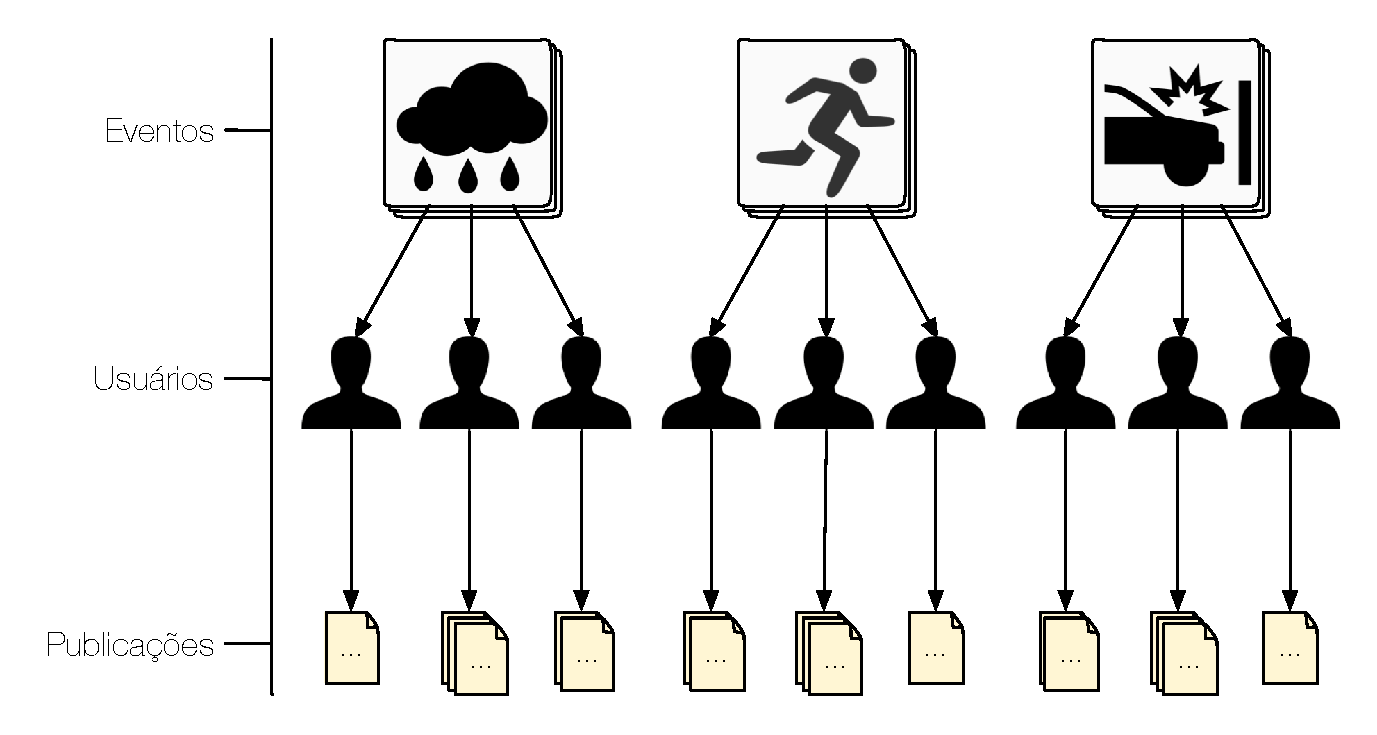
\includegraphics[width=0.85\textwidth]{figuras/event-perception-2.eps}
		\caption{O usuário como sensor de eventos do mundo real.}
	\end{center}
\end{figure}

Apesar da característica principal dos SNS ser a possibilidade dos usuários se relacionarem, cada serviço possui suas características específicas. Os principais serviços da atualidade são Twitter, Facebook Google+, etc.

\subsubsection*{Twitter}

O Twitter é um serviço de microblog aonde os usuários interagem entre si compartilhando publicações de texto limitadas até 140 caracteres. A principal característica do serviço é o dinanismo das publicações e a sua facilidade de compartilhamento. O dinanismo do serviço é explicitado pela funcionalidade de \textit{trending topics} (assuntos do momento), aonde estão ranqueados os termos mais comentados do momento, sendo atualizado várias vezes por dia.

A principal forma de interagir com outros usuários no Twitter através do recurso \textit{seguir}. Ao seguir um usuário, você passa a receber todas as suas publicações na sua página de \textit{linha do tempo}. A linha do tempo é principal página de interação com o sistema, aonde são exibidas todas as publicações dos usuários que você segue. Para cada publicação é possível \textit{curtir} (gostar publicamente), responder ou \textit{retweetar} (publicar novamente a mensagem para os usuários te seguem). Na Figura 2.2 está apresentada a linha do tempo de um usuário. No primeiro bloco da coluna da esquerda estão as informações do usuário ``Augusto'', sua quantidade de publicações, quantoas pessoas ele segue e quantas estão o seguindo. No segundo bloco estão os \textit{assuntos do momento}. Na coluna da direita se encontra a \textit{linha do tempo}.

\begin{figure}[htpb]
	\begin{center}	
		\includegraphics[width=0.8\textwidth]{figuras/twitter-main-screen.eps}
		\caption{Página principal do Twitter: linha do tempo.}
	\end{center}
\end{figure}

Hoje, com mais de 500 milhões de usuários registrados, o serviço criado em 2006 por Jack Dorsey cresce exponencialmente e tem ganhado atenção em várias frentes de pesquisas acadêmicas, exatamente por sua característica de troca de informações em tempo real. O trabalho de \citeonline{Java2007} apresenta a formação de comunidades e qual a motivação das pessoas ao utilizarem os serviços de microblogs e o Twitter, e concluiu que essa forma de interação induz à alta reciprocidade e correlação, indicando um entendimento mútuo entre os usuários e a facilidade de pulverização de informação. \citeonline{Jansen2009} estudaram o uso do Twitter como uma ferramenta de transferência de informação de pessoa para pessoa e analisou que o Twitter é uma das peças chave para o monitoramento de informação. \citeonline{Matuszka2013} analisam o ciclo de vida de cada palavra-chave com fim de detectar eventos, e enfatizam que o aparecimento de eventos específicos em redes sociais podem surgir antecipadamente aos outros meios de comunicação. \citeonline{Gao2014}, em seu trabalho, estuda o Twitter e os assuntos do momento, e uma forma de sumarizá-los e de retenção de informações e histórias, para que elas não se percam devido à intensa criação de informações proporcionada pelo serviço. 

O Twitter possui interfaces abertas para que aplicações externas sejam criadas. É possível através de serviços externos publicar por um usuário, ver todas as suas publicações, gostar de uma publicação, entre diversas outras ações. Através das interfaces, também é possível a busca por palavras-chave, o que torna o Twitter um serviço interessante para aplicação de diversas técnicas. Com ela é possível que serviços externos façam buscas complexas e recebam, em tempo real ou não, as publicações criadas por usuários correspondentes à essa busca. Tornando possível que se obtenha uma enorme quantidade de publicações para que sejam feitas análises de forma automatizada de dados, como a detecção de eventos.

\subsubsection*{Facebook}

O Facebook é o serviço de rede social mais popular da atualidade, e conta com cerca de 1.3 bilhão de usuário únicos\footnote{http://www.statisticbrain.com/facebook-statistics/}. O serviço possui várias maneiras de ser utilizado, ultrapassando o âmbito da conexão entre amigos e familiares. Além de ser possível criar seu perfil, compartilhar e visualizar publicações de texto, fotos e vídeos e criar amizades (conexões) com amigos, familiares e colegas de trabalho, o serviço oferece também a possibilidade da criação de páginas específicas para estabelecimentos comerciais, figuras famosas, organizações não governamentais etc. Também é possível a criação de eventos e convidar amigos, grupos privados e secretos e uma gama de outras coisas.

O serviço foi criado por Mark Zuckerberg em 2004 e vem crescendo rapidamente todos os anos. Hoje, cerca de 3 milhões de publicações são enviadas a cada 20 minutos e 2 milhões de novas conexões entre amigos são solicitadas\footnote{http://www.statisticbrain.com/facebook-statistics/}. O Facebook é, sem dúvida, a rede social com mais atividade entre seus usuários.

O Facebook possui a poderosa interface para desenvolvedores chamada Graph API, que é a principal ferramenta com que se interage de forma sistêmica com o serviço. É uma interface baseada em HTTP que pode ser utilizada para consultar dados, realizar publicações, subir fotos, etc. A Graph API é baseada em três princípios\footnote{https://developers.facebook.com/docs/graph-api/quickstart/v2.0}:

\begin{itemize}
	\item \textbf{Nós:} Entidades como Usuário, Foto ou Comentário.
	\item \textbf{Bordas:} As conexões entre as entidades, como fotos de um usuário, ou comentários de uma foto.
	\item \textbf{Campos:} Informações sobre as entidades, como o nome de um Usuário ou data de criação de uma foto.
\end{itemize}

A Graph API, porém, não permite com que sejam consultadas as publicações no serviço no âmbito geral, ou seja, com ela é possível apenas buscar as publicações ou realizar atividades relacionadas à um usuário em específico. Para realizar buscas por publicações através de palavras-chave, por exemplo, é necessário utilizar a \textit{Keyword Insights API} ou a \textit{Public Feed API}, porém, essas APIs são liberadas apenas para um conjunto específico de editores de mídia e não é possível, atualmente, conseguir chave para utilização das mesmas.

\subsubsection*{Google+}

O Google+ (Google Plus) é o serviço de rede social criado pelo Google Inc. em 2011. Hoje, após a incorporação dos usuários de outros serviços do Google como Gmail e Orkut, o serviço conta com uma base de cerca de 1.1 bilhão de usuários\footnote{http://socialmediaslant.com/google-plus-traffic-stats-february-2014/}.

O Google+ possui muitas das suas funcionalidades inspiradas no serviço Facebook, seu principal concorrente, porém com o diferencial de ser baseado em círculos de amizade. Nos círculos você pode compartilhar publicações apenas para um determinado grupo de amigos ou familiares, além de permitir a melhor organização de todas as pessoas que conhece. 	

O serviço possui interface para desenvolvedores chamada \textit{Google+ API}, que é possível com que se integre aplicativos e sites com o mesmo, podendo realizar publicações, criar amizades, obter informações de usuários, etc. Porém, possui a limitação de que apenas é possível buscar informações relacionadas à um usuário em específico e suas ligações. O serviço não disponibiliza uma interface com que seja possível buscar publicações de modo geral, como o Twitter oferece.

\section{Métodos de detecção de eventos}

Os métodos para implementação da técnica da detecção de eventos podem ser categorizados em métodos estatísticos, métodos probabilísticos e métodos de aprendizado de máquina. Segundo \citeonline{Jiang2009}, embora existam outros métodos que não se encaixam nessas categorias, a maioria pertence à uma ou mais delas.

\subsection{Métodos estatísticos}

O método estatístico mais simples consiste na aplicação de um \textit{limiar} superior ou inferior em que, caso o dado vindo do sensor chegue a esse limiar o evento é detectado, como no caso do velocímetro do carro. Porém, os valores observados geralmente dependem dos valores passados, necessitando de métodos que representem esses estados passados e possam fazer previsões futuras, como os métodos de \textit{regressão}, \textit{séries temporais} e \textit{filtro de kalman}.

No método de análise e modelagem de \textit{regressão}, a variável dependente (Y) é modelada como uma função de variáveis independentes (X) e um termo de erro, que representa a variação da variável dependente que não pode ser explicada pelo modelo. O modelo de regressão linear é expressado pela Figura 2.3, em que os pontos são os valores exatos da variável dependente (Y) e a reta significa a aproximação estatística por regressão linear. Porém, quando quando a relação entre a variável dependente e a independente é observadamente não-linear, é necessário criar modelos de regressão não-lineares.

\begin{figure}[htpb]
	\begin{center}
		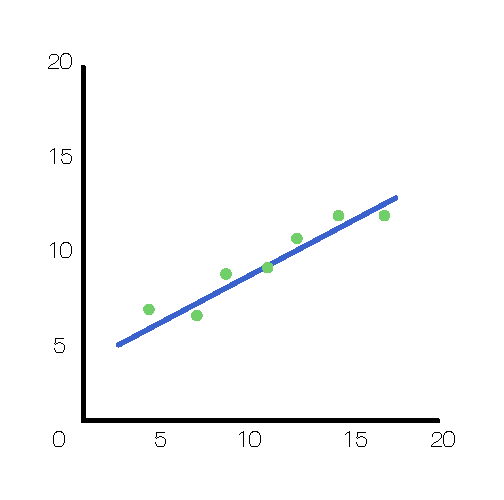
\includegraphics[width=0.4\textwidth]{figuras/regressao-linear.eps}
		\caption{Modelo de regressão linear.}
	\end{center}
\end{figure}

O método de \textit{séries temporais} consiste na modelagem estatística de dados que são medidos sucessivas vezes, com o mesmo intervalo de tempo entre as medições. O método tem como objetivo modelar os processos estocásticos subjacentes aos dados encontrados, para poder prever o valor de um estado futuro ou passado.

O \textit{filtro de Kalman} é um método estatístico recursivo criado por Rudolf Kalman que utiliza das medições ao longo do tempo para gerar predições que se aproximem de estados futuros e passados.

\subsection{Métodos probabilísticos}

Métodos probabilísticos, ao invés de analisarem e testarem amostras de dados como nos métodos estatísticos, consistem na estimativa da probabilidade da ocorrência de um evento e outras probabilidades e parâmetros relacionados. Existem diversos modelos e distribuições probabilísticas, como as de \textit{Poisson} e de \textit{Bernoulli}.

O modelo de \textit{Poisson} é utilizado quando se deseja calcular a probabilidade a ocorrência de um evento em um determinado espaço de tempo, sendo que os mesmos ocorrem independentemente e que a probabilidade de um evento ocorrer não muda através do tempo.

O modelo de \textit{Bernoulli} é utilizado quando os recursos analisados são binários, como por exemplo, a presença ou ausência mesmo. O modelo calcula a probabilidade de uma saída pertencer à uma classe ou outra.	

\subsection{Métodos de aprendizado de máquina}
	
Os métodos de aprendizado de máquina são geralmente utilizados quando os sensores são distruibuídos de forma esparsa no espaço e no tempo. Esses métodos geralmente recebem grandes volumes de informação e requerem alto poder computacional. Alguns exemplos são os \textit{filtros de partículas} e \textit{máquina de vetores de suporte}.

Os \textit{filtros de partículas} são algoritmos de aproximação probabilística que implementam o filtro Bayes. Em eventos, a técnica é utilizada para a estimativa de localização através de distruibuições probabilísticas que se propagam no tempo. Para isso, são geradas hipóteses (partículas) da localização de acordo com a distribuição dos dados. Por exemplo, para determinar a posição de um avião no espaço, sabendo sua posição em relação ao solo e a topologia do solo, o algoritmo, baseando-se nessas informações, gera inúmeras hipóteses de onde o avião possa estar. No próximo instante de tempo, sabendo a velocidade do avião e a sua direção, as possibilidades são atualizadas, até que as hipóteses convergirem para um valor considerado aceitável.

As \textit{máquinas de vetor de suporte} (SVM: \textit{support vector machines}) são algoritmos de aprendizado de máquina utilizados para a classificação de dados, que os analisam e reconhecem padrões. Eles são capazes de classificar futuras entradas a partir da análise de um conjunto de dados amostra previamente classificados.

No SVM, cada nova entrada de dados é representada como um ponto em um espaço, em que a técnica consiste em achar a divisão desses pontos que possui a maior margem possível entre eles, indicando assim a separação das duas classes. Na Figura 2.4 está ilustrada a maneira com que um SVM linear classifica as entradas de dados em dois grupos, porém esta classificação não é geralmente feita em um espaço de duas dimensões, e sim em um espaço de altíssima dimensão, podendo ser também feita de forma não-linear.

\begin{figure}[htpb]
	\begin{center}
		\includegraphics[width=1.0\textwidth]{figuras/svm-two-dimensional-field.eps}
		\caption{Classificação de um SVM: maior margem possível entre os dois grupos.}
	\end{center}
\end{figure}

Os SVMs são muito utilizadas para a detecção de eventos em documentos de texto, por funcionarem bem com um grande número de recursos, poucos recursos irrelevantes, dados esparsos e por conta da maioria dos problemas de classificação de texto serem lineares \cite{Joachims1998}.

\section{Classificação de texto}

A detecções de eventos em documentos de texto se apoia na técnica de \textit{classificação de texto}, que consiste na categorização de documentos em grupos aplicando um conjunto de técnicas que podem ser variadas, de acordo com o problema em questão. Segundo \citeonline{Aggarwal2012}, a classificação de texto pode ser aplicada nas mais variadas áreas, como:

\begin{itemize}
	\item \textbf{Organização e filtro de notícias:} Portais de notícias nos quais existe a criação de um grande volume de artigos todos os dias utilizam a classificação de texto - chamado nessa área também de filtragem de texto - para categorizar e filtrar os artigos de forma automatizada, pois em muitos casos a organização manual é inviável.
	\item \textbf{Organização e obtenção de documentos:} Muitos métodos de classificação de texto podem ser aplicados também em outras áreas, como bibliotecas digitais, literatura científica e publicações de redes sociais, com o fim de organizar os documentos de texto e facilitar sua futura obtenção.
	\item \textbf{Mineração de opinião:} A técnica pode ser aplicada para revisar avaliações de consumidores, geralmente pequenos textos, para determinar informações importantes para as empresas interessadas.
	\item \textbf{Classificação de email e filtro de spam:} A técnica pode, também, ser aplicada para classificar emails, para determinar se o email em questão é relevante ou apenas spam.
\end{itemize}

Os algoritmos para a classificação de texto precisam ser capazes de lidar com grandes quantidades de dados. Os textos podem ser modelados de acordo com suas palavras e as frequências das mesmas, logo, os algoritmos devem suportar dados que são esparsos, de alta dimensão e com baixa frequência na maioria das palavras. 

A maioria dos métodos de detecção de eventos podem ser encontrados e aplicados na classificação de texto. Segundo \citeonline{Aggarwal2012}, além das \textit{máquinas de vetores de suporte}, outros métodos mais utilizados são:

\begin{itemize}
	\item \textbf{Árvores de decisão:} As árvores de decisão são implementados criando uma divisão hierárquica dos textos, de acordo com os recursos especificados previamente. De acordo com cada recurso, é escolhido se o texto se enquadra no mesmo ou não, sendo possível, então, determinar à qual classe o texto pertence.
	\item \textbf{Classificadores baseados em padrões:}	Os classificadores baseados em padrões são implementados separando os textos em classes de acordo com seus padrões de palavras. Cada padrão de palavras aponta para uma classe, e esses padrões são utilizados para a classificação.
	\item \textbf{Classificadores Bayesianos:} Os classificadores bayesianos são classificadores probabilísticos baseados nos recursos de palavras de cada classe. Os textos analisados são classificados de acordo com a probabilidade deles pertencerem à uma classe específica.
\end{itemize}

A representação dos documentos e a seleção de recursos são questões importantes para a implementação dos métodos para classificação de texto. 

Os documentos podem ser representados como um conjunto de palavras, não importando a sua ordem, ou um conjunto de frases, em que cada documento é uma sequência de palavras. A maioria dos métodos de classificação de texto utilizam os documentos como um conjunto de palavras, por sua simplicidade de implementação.

A seleção dos \textit{recursos} pode ser feita através da remoção de palavras-filtradas (\textit{stop-word removal}) ou da redução de palavras-filtradas (\textit{stop-word stemming}). No primeiro, as palavras que não indicam as diferentes classes são removidas. No segundo, as palavras que possuem alguma relação pré-definida são reduzidas à apenas uma palavra, como remoção de plurais e de prefixos ou sufixos.

\section{Trabalhos Relacionados}

Os trabalhos de detecção de eventos encontram aplicação nos mais variados âmbitos. Muitos trabalhos aplicaram métodos estatísticos para comparar os resultados entre seus modelos e as atuais medições dos sensores como forma de detectar eventos anômalos. Outros aplicaram métodos probabilísticos para categorizar as medições em grupos de interesse. Outros utilizaram métodos de aprendizado de máquina para treinar e categorizar futuras ocorrências. E muitos outros aplicaram uma ou mais dessas técnicas no âmbito do Twitter.

\citeonline{Gupchup2009} utiliza a técnica de Análise de Componente Principal (PCA) para construir um modelo que é capaz de coletar as tendências das medidas de uma rede de sensores sem fio, e então são analisadas as diferenças entre o modelo e as reais medidas dos sensores para detectar anomalias. \citeonline{Hong2014} utilizam a detecção de eventos para detectar intrusos em redes de computadores. \citeonline{Zleikha2014} desenvolvem um algoritmo de decisão de floresta aleatória (random forest) para detectar eventos em dados vocais. Os eventos em questão podendo ser momentos de silêncio, risadas, etc.

\citeonline{Soule2005} desenvolveram um detector de eventos para detectar anomalias em redes de larga escala como empresas ou provedores utilizando filtro de kalman para filtrar o tráfego de rede comum e, para o tráfego remanescente são aplicadas quatro técnicas. Uma foca no comportamento instantâneo, outra na mudança da média do tráfego remanescente, a terceira em mudanças o comportamento da variância e a quarta nas mudanças da variância em múltiplas escalas de tempo.

No trabalho de \citeonline{Ihler2006} é construído um modelo de Poisson variável no tempo para detectar eventos anômalos em dados de contagem de séries temporais. A utilidade do modelo é demonstrada em dois âmbitos, dados de rodovias e de acessos à construções, e observa que o modelo possui melhor performance que um modelo não-probabilístico baseado em limiar. Os resultados indicaram que o modelo fornece uma robusta e precisa ferramenta para aprendizado autônomo e adaptável para separar eventos não usuais de atividades normais.

O trabalho de \citeonline{Sakaki2010} desenvolveu um algoritmo que detecta terremotos e tufões no Japão através das publicações coletadas do Twitter. As palavras ``terremoto'' e ``tremendo'' são utilizadas como palavras-chave, e foi utilizado o método de aprendizado de máquina \textit{máquina de vetores de suporte} com o kernel linear. O conjunto de amostras inicial que alimentou o SVM para a análise semântica foi composto por 597 publicações e depois da aquisição de resultados positivos, a localização e o horário de um terremoto são estimados utilizando os métodos probabilisticos filtro de kalman e filtro de partículas. Como resultado foi produzida uma notável aplicação, que detecta 96\% dos terremotos com escalas de intensidade 3 ou maior no território do Japão.

Um sistema que monitora publicações e detecta ocorrências de rinite alérgica no Japão foi desenvolvido por \citeonline{Takahashi2011}. A aplicação monitora publicações que contém a expressão ``hay fever'' (rinite alérgica) enviadas ao Twitter e utiliza o algoritmo AdaBoost.SDF, criado por \citeonline{Iwakura2008}, para classificar as publicações. Foi necessária a utilização do dado da localização do perfil do usuário para estimar a localização das publicações, e a normalização do número de publicações para cada região do Japão também foi necessária, pois percebeu-se que o número de publicações criadas em regiões em que o Twitter era popular era muito superior à outras áreas. Ao analisar a correlação entre os dados obtidos pelos sensores sociais e pelos sensores já utilizados, \citeonline{Takahashi2011} chegaram a conclusão de que o Twitter pode ser utilizado, neste caso, como uma alternativa aos sensores já existentes.

Um trabalho de investigação foi feito por \citeonline{Mai2012}, que analisou se as publicações enviadas ao Twitter pode ser uma fonte de dados para acidentes de transporte. O trabalho utiliza a API de transmissão em tempo real do Twitter para detectar publicações relevantes contendo palavras-chave como ``acidente'', ``batida'', ``rodovia'' e apenas as publicações contendo a localização geográfica do usuário foram selecionadas. Essas publicações são então comparadas com o os dados do orgão da Califórnia \textit{California High Patrol} utilizando os métodos de comparação baseado em volume e semântico. Concluiu-se que existe correlação entre os dados extraídos das publicações analisadas e os dados do órgão da California, porém um sofisticado filtro de conteúdo e localização se mostrou necessário para maximizar a relevância dos dados.

\citeonline{Wang2013} desenvolveram um algoritmo para a detecção de palavras que erupcionam repentinamente no Twitter. As palavras são obtidas através da interface para desenvolvedores \textit{Streaming API}. É utilizado o pré-processamento de palavras para remover replicações como risadas ou onomatopéia. A remoção de palavras de filtragem é utilizada e publicações com menos de duas palavras também são filtradas. É utilizado um probabilístico de mistura Gaussiano para a extração das palavras que erupcionam e para a detecção de evento. Finalmente, para o reconhecimento da localização é utilizado um modelo probabilístico de campo aleatório condicional (CRF: \textit{conditional random field}).

\section{Discussão das técnicas}

\citeonline{Wang2013} utiliza a interface para desenvolvedores do Twitter \textit{Streaming API}, porém, optamos por utilizar a interface \textit{REST API} pois com ela é possível obter publicações mais antigas e não necessitar da manutenção de uma conexão que fique sempre ativa. A \textit{Streaming API}, como é um serviço de tempo real, aceita apenas novas obtenções de publicações a partir do momento seguinte à conexão.

Os trabalhos de \citeonline{Sakaki2010}, \citeonline{Mai2012} e \citeonline{Takahashi2011} aplicam a detecção em eventos de alto impacto como desastres naturais, acidentes de transito e doenças. Escolhemos aplicar a técnica para a detecção de eventos de manifestações por possuir características semelhantes como geração de impacto, revolta e ser um evento anômalo ao funcionamento comum da sociedade de modo geral.

Obtou-se pela utilização do SVM como classificador de texto por demonstrar alta recorrência em trabalhos como \citeonline{Santos2010}, \citeonline{Pak2010}, \citeonline{Benevenuto2010}, \citeonline{Go2009}, entre outros.
\chapter{Detecção de eventos através do Twitter}

O Twitter possui um imenso banco de dados de publicações criadas por usuários, tornando-se uma fonte para aplicação de técnicas de análise de texto. Além do texto propriamente dito de cada publicação, o serviço também armazena dados úteis como o horário em que a ela foi criada e a localização do usuário ao criá-la.

O serviço disponiliza as informações das publicações através de interfaces de aplicação, para que aplicações externas possam realizar buscas de forma automatizada, além de outras ações. O modelo de detector de eventos proposto utiliza as publicações disponibilizadas pelo Twitter como fonte de dados para detectar ocorrências de manifestações. O detector se apoia nas informações criadas por seus usuários para retirar informações relevantes como o local e o horário de manifestações.

Para validar o detector de eventos proposto, o modelo busca por publicações que contém a palavra-chave ``manifestação'', criadas no mês de Agosto de 2014. Todas as publicações contendo a palavra-chave são copiadas para um ambiente de trabalho local. 

As publicações obtidas, porém, não passam por filtros ao serem criadas e diversas delas devem ser descartadas para o processo de detecção. Mesmo contendo a palavra-chave buscada, muitas podem não dizer respeito ao evento que o modelo deseja detectar. Para classificar as publicações que são relevantes para o modelo e as que devem ser descartadas, o modelo utiliza a técnica de aprendizado de máquina SVM como \textit{classificador de texto}. 

O SVM é um método de aprendizado supervisionado em que, através de um conjunto inicial de exemplos previamente classificados, consegue induzir em qual classe uma nova ocorrência se encaixa. O modelo utiliza um conjunto de \textit{publicações de treino}, previamente classificadas entre ocorrências positivas, ou seja, indicam a ocorrência real de um evento de manifestação, e negativas, não indicam a ocorrência, podendo ser apenas o termo empregado em outro contexto, ser referente à uma manifestação futura ou passada, etc. Esse processo é chamado de \textit{representação do conhecimento}, que é quando o conhecimento do ambiente (publicações sobre manifestações) é passado para a máquina de aprendizado, que analisa os padrões das informações e adquire o conhecimento.

Com o conhecimento representado, o SVM pode classificar novas ocorrências. Porém, o SVM não recebe como entrada o texto das publicações, e sim a sua representação matemática. O modelo implementado representa os textos no \textit{modelo de espaço vetorial}, aonde eles são convertidos para um vetor que contem as informações relacionadas à presença ou ausência de seus termos. Para converter, as publicações são divididas em termos, separados por espaço, e é criado um dicionário dos termos de todas as publicações. Através dessa representação, o SVM realiza operações matemáticas que determinam as relações de distância entre os dados, podendo inferir à qual classificação cada dado se enquadra.

Após a classificação das publicações, o modelo extrai o horário e a localização das publicações positivas. A informação do horário será utilizada para agrupar as publicações, com o intuito de determinar os horários em que ocorreram mais ocorrências de menções à manifestações. Os horários de pico representam os \textit{eventos}, que são ocorrências anômalas ao funcionamento normal do fluxo contínuo de publicações. Já a localização será utilizada para a analise visual das regiões de ocorrência dos eventos, que serão traçadas nos mapas apresentados. A arquitetura proposta é ilustrada na Figura 3.1.

\section{Publicações como fonte de dados}

No Twitter, cerca de 500 milhões de publicações\footnote{http://www.internetlivestats.com/twitter-statistics/} são criadas diariamente, e junto com elas, diversos dados úteis são gravados. Uma publicação é o conjunto de dados de uma mensagem que é enviada ao servidor do Twitter. Cada texto de uma publicação é limitado a 140 caracteres, e possui também dados adicionais como:

\begin{itemize}
	\item Horário de criação
	\item Idioma
	\item Dados do usuário que a publicou como nome, localização, descrição e foto
	\item Geolocalização (para envios de smartphones, tablets e notebooks com essa opção ativada)
	\item Referências à links, usuários e hashtags, caso possuam
	\item Publicação na qual está respondendo 
\end{itemize}

\begin{figure}[htpb]
\begin{center}
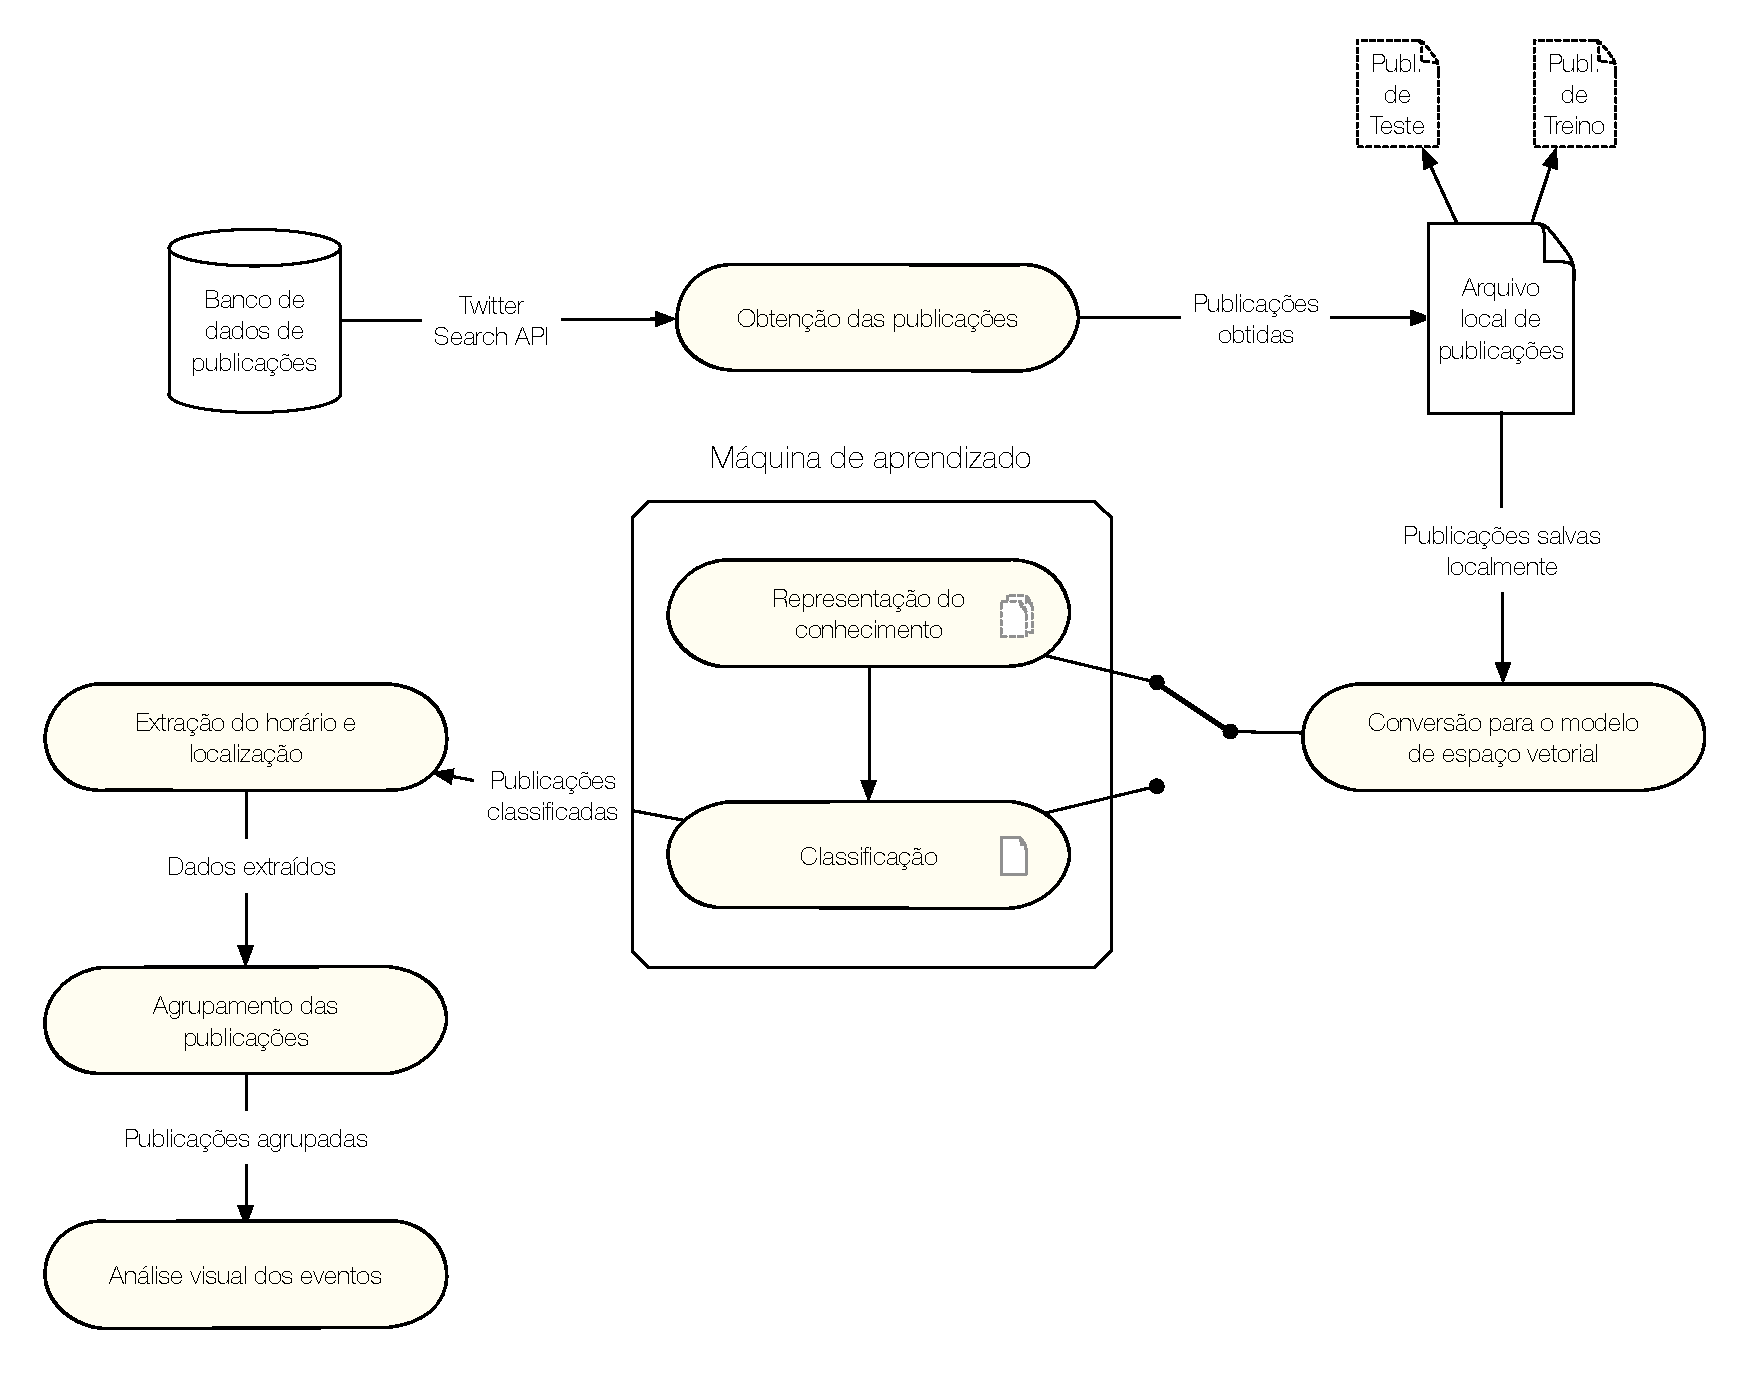
\includegraphics[width=1.0\textwidth]{figuras/fluxograma-deteccao.eps}
\caption{Processo de detecção para o detector de eventos proposto.}
\end{center}
\end{figure}

As publicações são criadas por usuários e dizem respeito aos mais variados eventos dos mundo real. Com o acesso à essas publicações é possível melhorar serviços externos, prever resultados de votações, monitorar opiniões sobre marcas, detectar desastres naturais etc. \citeonline{Tumasjan2010}, por exemplo, acham um grande paralelo entre o sentimento político dentro das publicações no serviço e fora do mesmo. \citeonline{Stankovic2010} criam uma ferramenta que mapeia as publicações que são referentes à conferências. Já \citeonline{Cox2011} utilizam as publicações referentes à observações sobre o clima para melhorar as previsões do tempo.

As publicações, por serem criadas por usuários, não passam por qualquer tipo de filtro, e grande parte delas devem ser descartadas para o sucesso das análises, seja por conter palavras com a grafia errada, gírias, ou por não dizerem respeito à qualquer conteúdo relevante. De acordo com a \citeonline{PearAnalytics2009}, aproximadamente 40\% das publicações não possuem relevância, atuando apenas como ruído para as análises.

Para o sucesso das técnicas de análise que utilizam publicações como dados de entrada, é necessário que o processo reconheça adequadamente as publicações que são apenas ruídos e as tratem, processem e/ou excluam, para que os resultados obtidos sejam relevantes e satisfatórios.

Na detecção de eventos, é preciso também que o evento contenha quantidade suficiente de publicações relacionadas. Apenas eventos com certa relevância podem ser detectados, pois caso contrário não haverá quantidade suficiente de publicações para gerar análises consistentes. Segundo \citeonline{Sakaki2010}, alguns fatores, como escala, influência e região, aumentam a probabilidade que um evento possa ser detectado no Twitter.

\begin{itemize}
	\item \textbf{Escala:} Eventos com grande escala são vivenciados por muitas pessoas, gerando uma maior quantidade de publicações.
	\item \textbf{Influência:} Eventos com maior grau de influência na vida dos pessoas tendem induzi-las mais a compartilhar a experiência e gerar publicações.
	\item \textbf{Região:} Eventos com região de espaço e tempo delimitados permitem que sejam feitas estimativas do horário e da localização.
\end{itemize}

Eventos de grande escala, com alto grau de influência e com região de tempo e espaço são os tipos de eventos mais propícios para a aplicação da detecção de eventos, pois geram um maior fluxo de publicações e permitem a estimativa da sua localização. Alguns exemplos de eventos com essas características são desastres naturais como terremotos, tempestades, ciclones e tufões, eventos sociais como grandes festivais, eventos esportivos e políticos e desastres não naturais como acidentes de todos os tipos.

A obtenção das publicacões é feita através das \textit{interfaces de aplicação} do Twitter, que disponibilizam seus dados através de uma formatação em texto estruturada.

\section{Interfaces para obtenção dos dados}

Para disponibilizar as publicações, o serviço utiliza a forma de notação JSON (\textit{JavaScript Object Notation}) para troca de dados. Uma formatação leve, em formato de texto, que permite que os dados das publicações sejam transferidos pela rede de internet para serviços externos. Os dados são estruturados em pares de nome/valor e possuem ordem fixa. O Código 3.1 apresenta a estrutura da uma publicação, com dados como data de criação, id, texto, etc.

\begin{lstlisting}[caption=Estrutura JSON de uma publicação]
	{
		:created_at=>"Thu Jul 31 15:14:27 +0000 2014",
	  :id=>494863667100258304,
    :text=>"Manifestacao deixa transito congestionado em Sao Cristovao: Funcionarios do transporte alternativo protestam...",
	  (...)
    :user=>{
    	:id=>2340427167,	
      :name=>"Rodrigo",
      :location=>"Sao Paulo",
      (...)
     },
    :geo=>nil,
    :coordinates=>nil,
    :place=>nil,
    (...),
    :lang=>"pt"
  }
\end{lstlisting}

Para transferir os dados, o Twitter disponibiliza interfaces de aplicação (APIs: \textit{Application Product Interfaces}) poderosas que permitem com que os desenvolvedores utilizem as informações disponíveis em seu serviço para os mais variados fins. São elas: \textit{Search API}, \textit{REST API} e \textit{Streaming API}\footnote{https://dev.twitter.com/start}.

\subsection*{REST API}

A \textit{REST API} é a interface mais básica do Twitter, que permite que desenvolvedores acessem as principais ações do serviço, como informações de usuários, atualizações de status e menções à um usuário específico. Além de permitir a criação de publicações, a resposta à outras publicações, o \textit{retweet} e que usuários as favoritem através de serviços externos. 

Uma das formas de utilizar a \textit{REST API} constitui em criar um servidor HTTP mediador das ações entre o usuário e o Twitter. O servidor recebe as ações do usuário em seu website, analisa a requisição e então a repassa para o Twitter para realizar qualquer ação necessária para enviar a resposta para o usuário. O website então atualiza sua página e o usuário vê as informações que pediu, como segue na Figura 3.2.

\begin{figure}[htpb]
	\begin{center}
	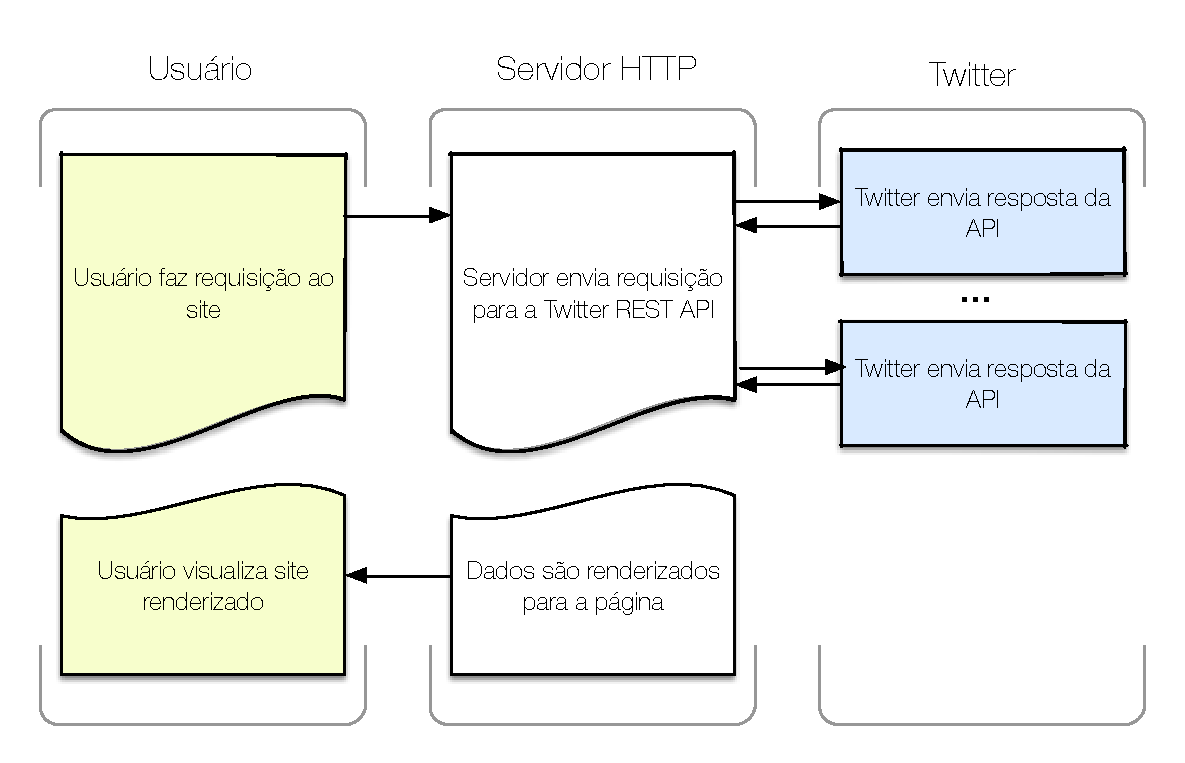
\includegraphics[width=0.8\textwidth]{figuras/twitter-rest-api.eps}
	\caption{Funcionamento da REST API do Twitter.}
	\end{center}
\end{figure}

\subsection*{Search API}

A \textit{Search API} faz parte da \textit{REST API} e é a interface do Twitter que serve com o propósito específico de buscar por publicações. Ela permite que desenvolvedores façam buscas por publicacões através de palavras-chave específicas, além de forneceder operadores para que a busca seja refinada. 

A \textit{Search API} é focada na relevância dos dados, não em sua totalidade, ou seja, apenas as publicações serão retornadas e existe um limite de resultados à serem retornados. Na Tabela 3.1 estão representados alguns dos operadores disponíveis.

\begin{table}[ht]
	\caption{Operadores da Search API}
	\centering
	\begin{tabular}{| l | l |}
		\hline
		\textbf{Operador} & \textbf{Busca por publicações contendo...} \\ [0.5ex] \hline \hline
    assistindo agora & contendo ``assistindo'' e ``agora'' \\
    ``chegando em casa'' & contendo exatamente a frase ``chegando em casa'' \\
    amor OR ódio & contendo ``amor'' ou ``ódio'' (ou os dois) \\
    amor -ódio & contendo ``amor'' mas não ``ódio'' \\
    \#copa & contendo a hashtag ``copa'' \\
    @mashable & referenciando o usuário ``mashable''  \\ 
    ... & ... \\ [1ex]
		\hline
	\end{tabular}
	\label{table:nonlin}
\end{table}

Por exemplo, buscando pelo termo ``estou aqui'', o serviço retorna todas as publicações com os termos ``estou'' e ``aqui'', independente da ordem e da posição das palavras na mensagem. Ao buscar pelos termos entre aspas, o serviço retorna as publicações contendo exatamente a expressão pesquisada. Existe também o operador lógico ``OR'', que retorna as publicações que contem uma palvavra ou a outra. Além da busca por \textit{hashtags} (\#) e menções aos usuários (@). Essas, porém, não constituem todas as buscas possíveis no serviço, sendo possível inclusive combinar os operadores\footnote{https://dev.twitter.com/docs/using-search}.

\subsection*{Streaming API}

A \textit{Streaming API} é a interface do Twitter que permite acesso de baixa latência e sem os limites da \textit{Search API}. Com ela, é possível fazer requisições em tempo real para o serviço, obtendo as publicações conforme são criadas.

Nessa API, o primeiro passo é solicitar uma conexão permanente (streaming) com o servidor do Twitter, que então aceita a sua solicitação e abre a conexão. O Twitter começa, então, a enviar as publicações de forma automática, conforme elas são criadas. O serviço que solicitou se encarrega de processá-las e guardá-las como for conveniente. O usuário então, ao acessar o serviço, faz a requisão e o serviço obtém os dados processados de seu banco de dados (não diretamente do Twitter) e renderiza a página para que o usuário possa visualizar os resultados, como explicitado na Figura 3.3.

\begin{figure}[htpb]
\begin{center}
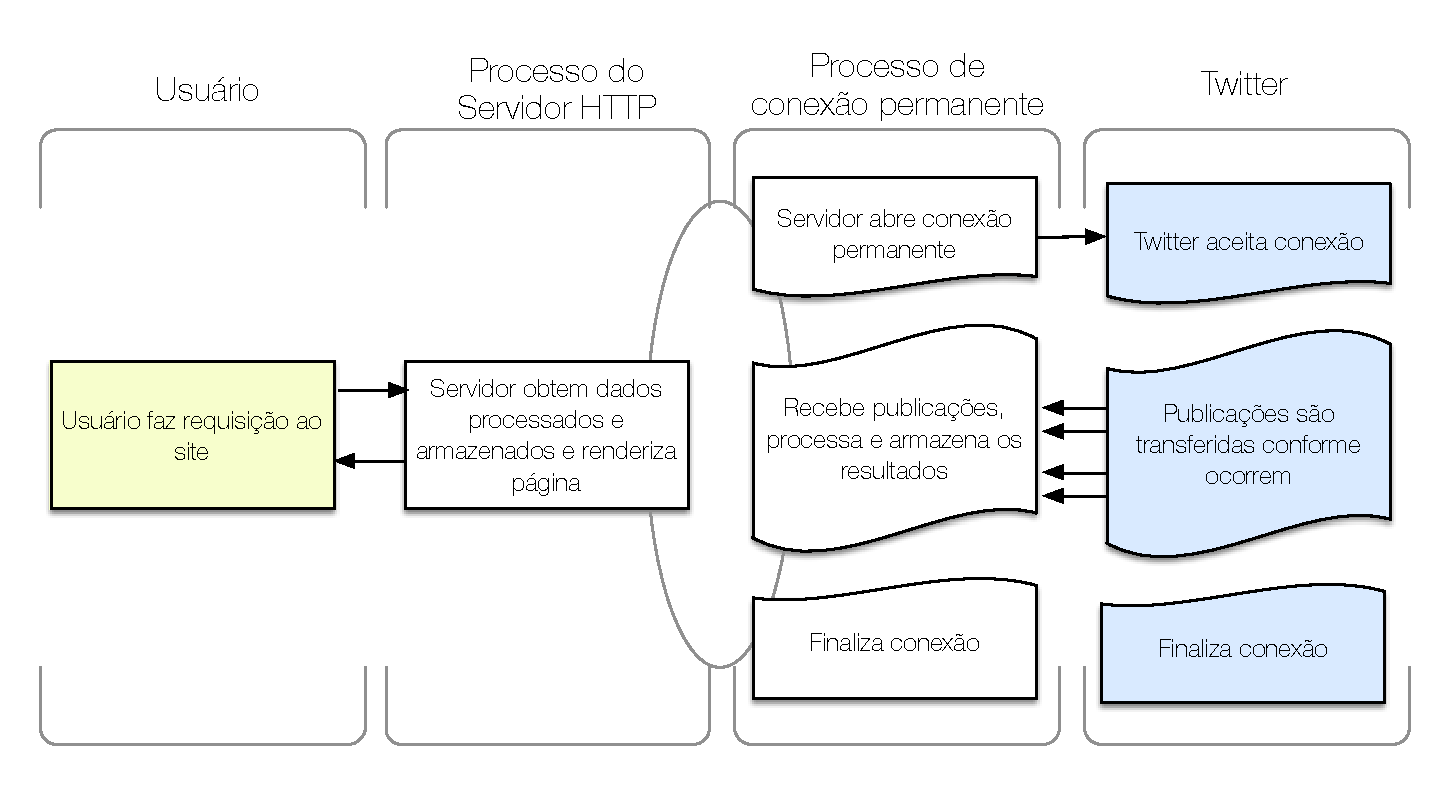
\includegraphics[width=1.0\textwidth]{figuras/twitter-streaming-api.eps}
\caption{Funcionamento da Streaming API do Twitter.}
\end{center}
\end{figure}

A elipse central da Figura 3.3 representa que os dois lados estão conectados, mas não de forma síncrona. Para o \textit{servidor HTTP} obter os dados processados, é necessário que, antes a \textit{conexão permamente} tenha sido criada e as publicações obtidas. Porém, o intervalo entre a obtenção das publicações e a requisição do usuário pode ser variado. É possível que a \textit{conexão permanente} já tenha sido terminada antes da requisição para o \textit{servidor HTTP}, ou também que os dois estejam agindo simultaneamente.

\section{Obtenção dos dados}

A primeira etapa para a implementação de um detector de eventos é a obtenção dos dados. Para o modelo implementado, os dados são obtidos do banco de dados do Twitter, através de sua interface para desenvolvedores. A interface permite que a informação trafegue pela rede através do formato de texto. Com a busca por uma palavra-chave específica, o serviço reune todas as publicações referentes à ela em um arquivo de texto e o envia de forma estruturada, para que localmente esses dados sejam tratados e salvos de várias maneiras.

O modelo utiliza a interface \textit{Search API} para buscar por publicações. Como o serviço informa, essa interface não disponibiliza a quantidade total de publicações criadas, e sim as mais relevantes - para ter acesso à todas as publicações é necessário utilizar a \textit{Streaming API}. Por isso, foram realizados testes para definir se a interface servia para o propósito do modelo. 

Os testes mostraram que a \textit{Search API} retorna quantidade relevante de publicações e elimina a necessidade da implementação de um servidor com conexão permanente com o Twitter, o que seria necessário para a utilização da \textit{Streaming API}. Caso o servidor caísse, seriam perdidas as publicações criadas nesse período, e não seria possível a busca por publicações anterior ao período de criação do servidor.

Para validar o modelo implementado, pretende-se detectar ocorrências de manifestações no território brasileiro no mês de Agosto de 2014. Para isso, é realizada a busca por publicações com a palavra-chave ``manifestação''. 

Como a interface utilizada retorna apenas publicações criadas há, no máximo, uma semana, torna-se necessário programar mais de uma busca, em diferentes datas. Após a obtenção dos dados estruturados das publicações em formato JSON, são selecionados os seguintes dados: 

\begin{itemize}
	\item Texto da publicação
	\item Horário de criação da publicação
	\item Latitude e longitude do usuário
	\item Localização configurada perfil do usuário
	\item Identificador único da publicação
\end{itemize}

O texto da publicação é a publicação propriamente dita, que serve com o propósito de detectar as ocorrências de manifestação. O horário de criação, a latitude e longitude e a localização configurada no perfil são utilizadas em passos posteriores para o agrupamento das publicações. O identificador único é útil para definir a última publicação buscada e definir, na próxima busca, em qual publicação a busca irá parar.

Os dados selecionados são gravados localmente em um arquivo CSV (\textit{comma separated values}), um formato de dados em texto em que os campos são separados por vírgulas. Os dados formam uma tabela, sendo as vírgulas delimitadoras das colunas e as quebra de linha delimitadoras de linhas. São adicionadas aspas nos campos para impedir que as vírgulas dos textos se confundam com as vírgulas separadoras dos campos. A Tabela 3.2 representa exemplos de publicações contidas no arquivo CSV.

\begin{table}[ht]
	\caption{Representação em tabela do arquivo CSV}
	\centering
	\begin{tabular}{| p{1cm} | p{2cm} | p{4cm} | p{2cm} | p{2cm} | p{2.5cm} |}
		\hline
		\textbf{Id} & \textbf{Horário} & \textbf{Texto} & \textbf{Latitude} &\textbf{Longitude} & \textbf{Localização perfil} \\ [0.5ex] \hline \hline
    49744 40914 21286 400 & 2014-08-07 14:45:23 & Aumento da passagem de ônibus provoca manifestação em sorocaba & -15.850902 & -47.944792 & Brazil \\ \hline
    49743 91868 07685 121 & 2014-08-07 14:40:19 & Grupo faz manifestação contra assassinatos de mulheres em goiânia &  &  &  \\ \hline
    49743 54381 48104 192 & 2014-08-07 14:39:50 & sabe se já acabou a manifestação??? &  &  & Rio de Janeiro - Brasil \\
    ... & ... & ... & ... & ... & ... \\
		\hline
	\end{tabular}
	\label{table:nonlin}
\end{table}

Com as publicações gravadas no arquivo CSV, são selecionadas algumas publicações para gerar dois outros arquivos: um que irá conter as \textit{publicações de treino} e outro que irá conter as \textit{publicações de teste}. Os novos arquivos terão o propósito de fornecer as publicações para representar o conhecimento para o SVM.

Após a obtenção das publicações, então, cada uma é convertida para o seu modelo de espaço vetorial, para que o SVM utilize a representação vetorial de cada publicação e possa classificá-las de acordo com suas características.

\section{Modelo de espaço vetorial}

O \textit{modelo de espaço vetorial} é um modelo de representação de dados em vetores de características. Os vetores são constituídos por termos de índice, que podem conter pesos de acordo com sua importância ou não \cite{Salton1975}. Os vetores são utilizados para analises estruturas e operações matemáticas a partir dos dados convertidos, o que não seria possível a partir dos dados originais, como documentos de texto. 

Para a conversão de dados para o modelo de espaço vetorial, são escolhidos em quais tipos de recursos ele é constituído. Os recursos, em documentos texto, podem ser um conjunto de termos separados por espaço, frases separadas por pontuação, quebra de linha, etc. Segundo \citeonline{Joachims1998}, os recursos provenientes de documentos de texto possuem as seguintes características:

\begin{itemize}
	\item \textbf{Alta dimensão:} Os recursos geralmente são as palavras presentes nos documentos, ou seja, podem chegar à altíssimas dimensões, uma vez que cada palavra será uma dimensão no vetor de recursos.
	\item \textbf{Poucos recursos irrelevantes:} Nos documentos de texto, poucos recursos são irrelevantes, mantendo a sua alta dimensão e impedindo que algoritmos classificadores baseados na remoção de recursos irrelevantes sejam utilizados.
	\item \textbf{Dados esparsos:} Para cada documento, o vetor de características correspondente contém apenas algumas entradas que não são zero, pois possui apenas alguns dos termos do dicionário.
\end{itemize}

O recurso escolhido pelo modelo implementado é a presênca ou ausência de palavras em cada publicação. Palavras são todas os conjuntos de caracteres separados por espaço, o que chamamos de \textit{termo}. Primeiramente, aplica-se a \textit{tokenização} nas publicações, para gerar os seus termos constituintes. Os termos passam, então, pelo \textit{pré-processamento}, que agrupa termos que possuem o mesmo significado, como palavras seguidas de pontuação e maiúsculas ou minúsculas. 

Todos os termos são então agrupados e ordenados em ordem alfabética, criando assim o \textit{dicionário de termos}. No dicionário, cada termo possui um identificador único, idêntico à sua ordem. Após a criação do dicionário, cada publicação é convertida para sua representação no modelo de espaço vetorial, aonde os seus vetores de características são extraídos de acordo com os termos presentes e o índice desses termos no dicionário. Na Figura 3.4 estão apresentadas as fases da conversão para o modelo de espaço vetorial.

\begin{figure}[htpb]
	\begin{center}
		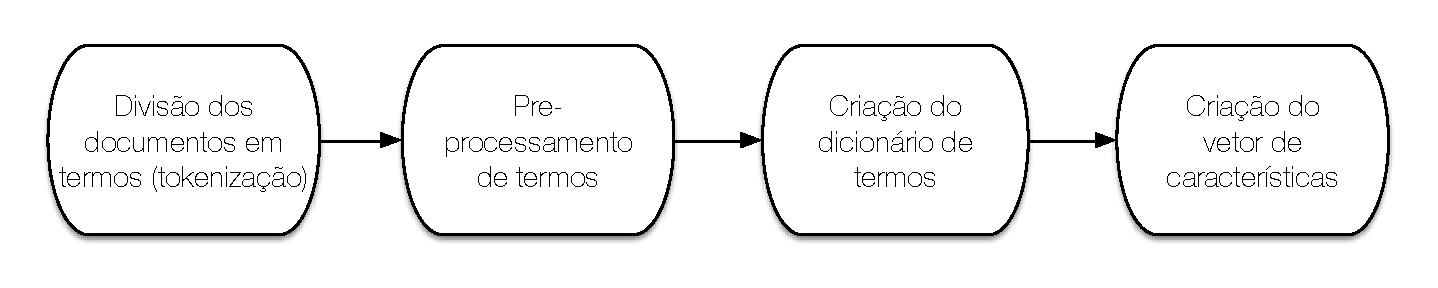
\includegraphics[width=1.0\textwidth]{figuras/processo-modelo-espaco-vetorial.eps}
		\caption{Processo de conversão para o modelo de espaço vetorial.}
	\end{center}
\end{figure}

\subsection{Tokenização}

A tokenização é o primeiro passo na conversão para o modelo de espaço vetorial, nela os documentos são convertidos em um conjunto de termos. Os delimitadores de termos podem ser espaços, pontuação, linhas, etc. Alguns processos de tokenização, pode ser mais complexos do que isso, por exemplo, como indicado por \citeonline{Turney2010}, alguns \textit{tokenizadores} devem ser capazes de reconhecer termos de mais de uma palavra, como ``Barack Obama'', termos que contém hífem e pontuação, ignorar pronomes e preposições, etc.

O modelo implementado utiliza espaços para delimitar os termos de cada publicação e utiliza uma lista de palavras muito recorrentes, como preposições, para ignorá-las na criação dos termos, como ``em'', ``no'', ``de'', etc. Links também não geram termos, ou seja, todos os termos que começam com ``http://'' são ignorados.

O processo de tokenização divide a publicação em um vetor de $n$ termos. Por exemplo, a publicação ``Manifestação em Goiânia!'' é transformada no conjunto de 3 termos: ``Manifestação'', ``em'', ``Goiânia!'', como indicado na Figura 3.5.

\begin{figure}[htpb]
	\begin{center}
		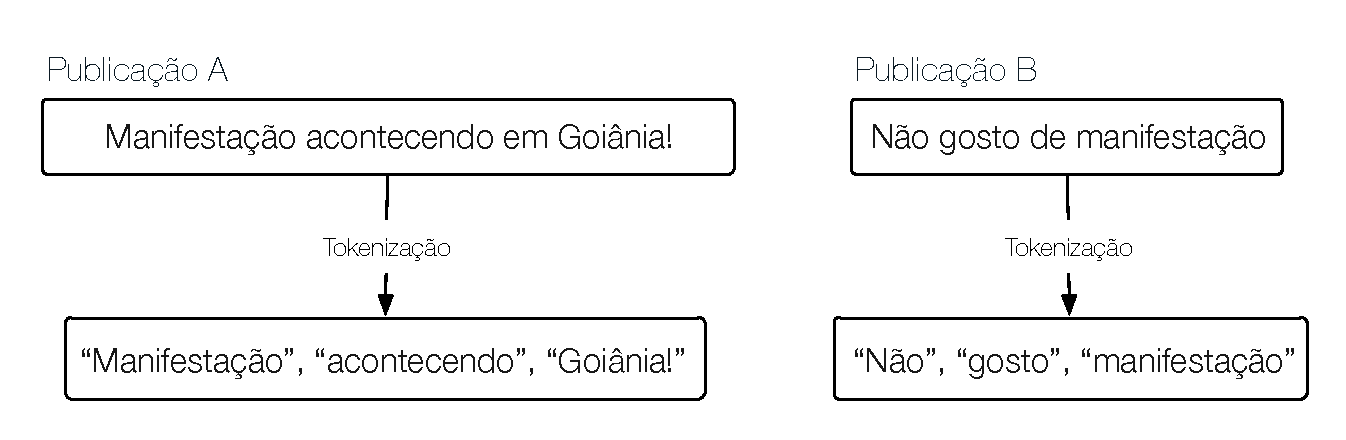
\includegraphics[width=1.0\textwidth]{figuras/tokenizacao.eps}
		\caption{Tokenização de duas publicações.}
	\end{center}
\end{figure}

A tokenização, porém, não trata de casos como o do termo ``Goiânia!''. Nesse caso, somente a pontuação e a letra maiúscula faz com que um novo termo seja criado, diferenciando-o de ``Goiânia'' e ``goiânia'', por exemplo. Isso adiciona complexidade à classificação, pois quanto mais termos, maior a dimensão dos dados a serem analisados. Para tratar desses casos, é necessário o \textit{pré-processamento} dos termos.

\subsection{Pré-processamento}

O pré-processamento é encarregado de normalizar os termos, para que não haja diferenciação entre termos que são essencialmente iguais. Isso diminui a complexidade da análise dos dados, na medida em que reduz a dimensão dos vetores de características.

No modelo implementado, os termos são pré-processados removendo suas pontuações e transformando-os para minúsculas. Ou seja, o pré-processamento retira a diferenciação de termos como ``manifestação'', ``Manifestação'' e ``manifestação.''. Todos os exemplos, após o pré-processamento, são identificados como o mesmo termo. Na Figura 3.6 é demonstrado o pré-processamento para duas publicações.

\begin{figure}[htpb]
	\begin{center}
		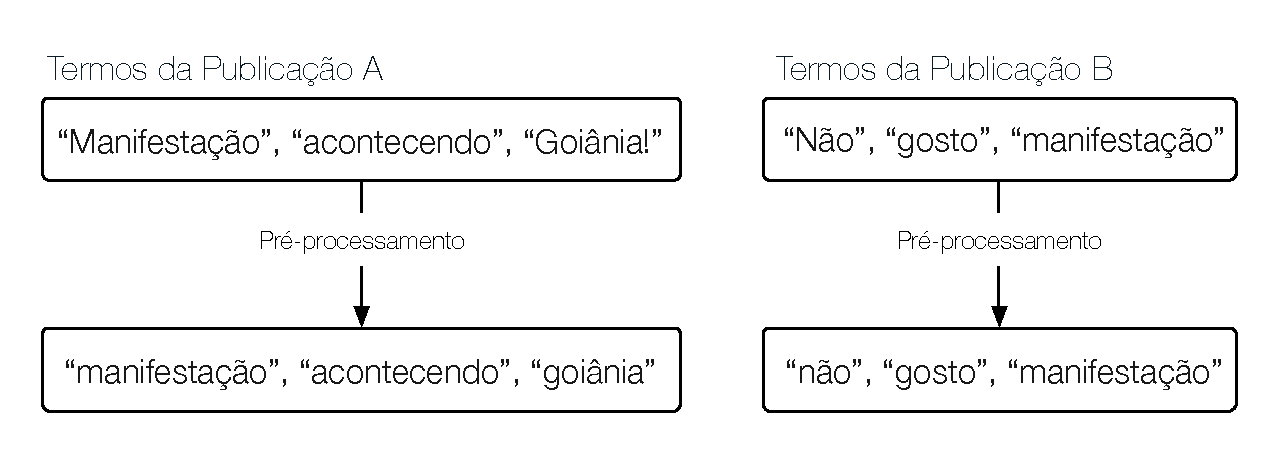
\includegraphics[width=1.0\textwidth]{figuras/pre-processamento.eps}
		\caption{Pré-processamento de duas publicações.}
	\end{center}
\end{figure}

\subsection{Criação do dicionário de termos}

Após pré-processados os termos, é criado um dicionário de todos os termos obtidos, o \textit{dicionário de termos}. No dicionário, os termos são únicos, não importando quantas vezes são repetidos no conjunto de publicações. Os termos são também ordenados em ordem alfabética, o que concede um identificador único para cada termo. O primeiro termo possui identificador ``0'', o segundo ``1'', e assim por diante.

A quantidade de termos do dicionário define a dimensão dos vetores de caraterísticas das publicações. Todos os vetores terão a dimensão da quantidade de termos no dicionário, e cada elemento do vetor representa um termo do dicionário. O primeiro elemento de cada vetor será referente ao primeiro termo do dicionário, e seu valor depende se a publicação contém o termo ou não. A Figura 3.7 representa um dicionário para duas publicações.

\begin{figure}[htpb]
	\begin{center}
		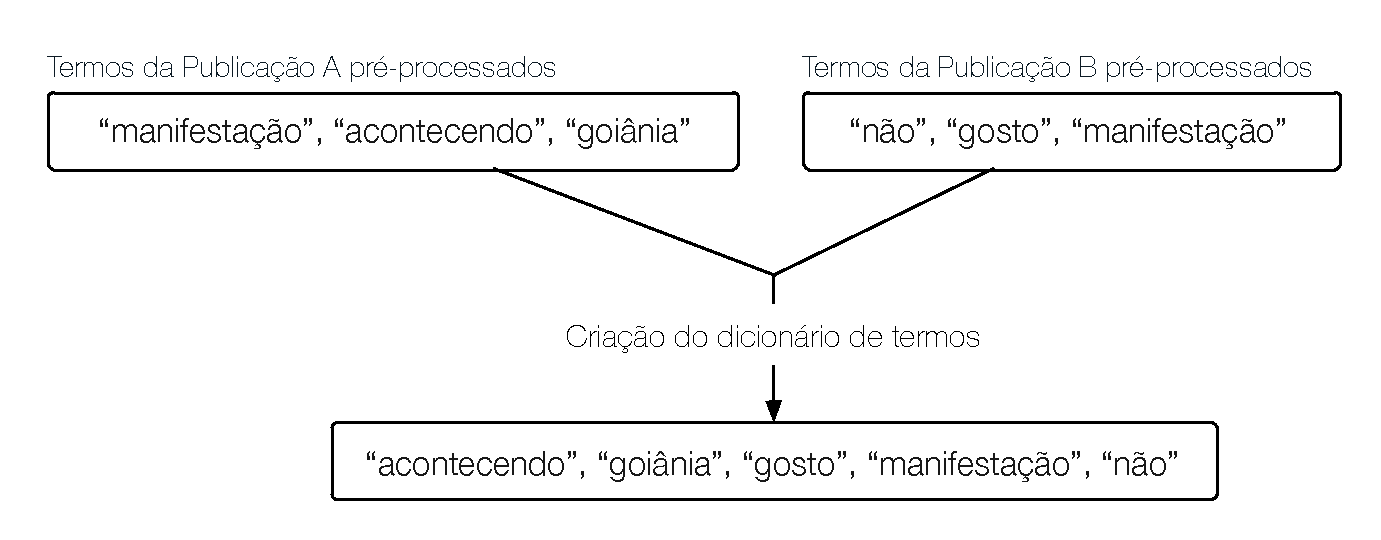
\includegraphics[width=1.0\textwidth]{figuras/dicionario-termos.eps}
		\caption{Dicionário de termos de duas publicações.}
	\end{center}
\end{figure}

\subsection{Criação do vetor de características}

À partir do dicionário, é possível a extração do vetor de características de cada publicação. O valor de cada elemento do vetor será ``1'' se a publicação contém o termo, ou ``0'' se a publicação não contém. Ou seja, se o primeiro termo do dicionário é a palavra ``gosto'', e o vetor é referente à publicação ``não gosto de manifestação'', a sua primeira posição será o valor ``1'', pois a publicação contém termo ``gosto''. Se o segundo termo for ``rua'', a segunda posição do vetor dessa publicação possuirá o valor ``0'', pois não possui o termo, e assim por diante. A Figura 3.8 representa a criação do vetor de características para duas publicações.

\begin{figure}[htpb]
	\begin{center}
		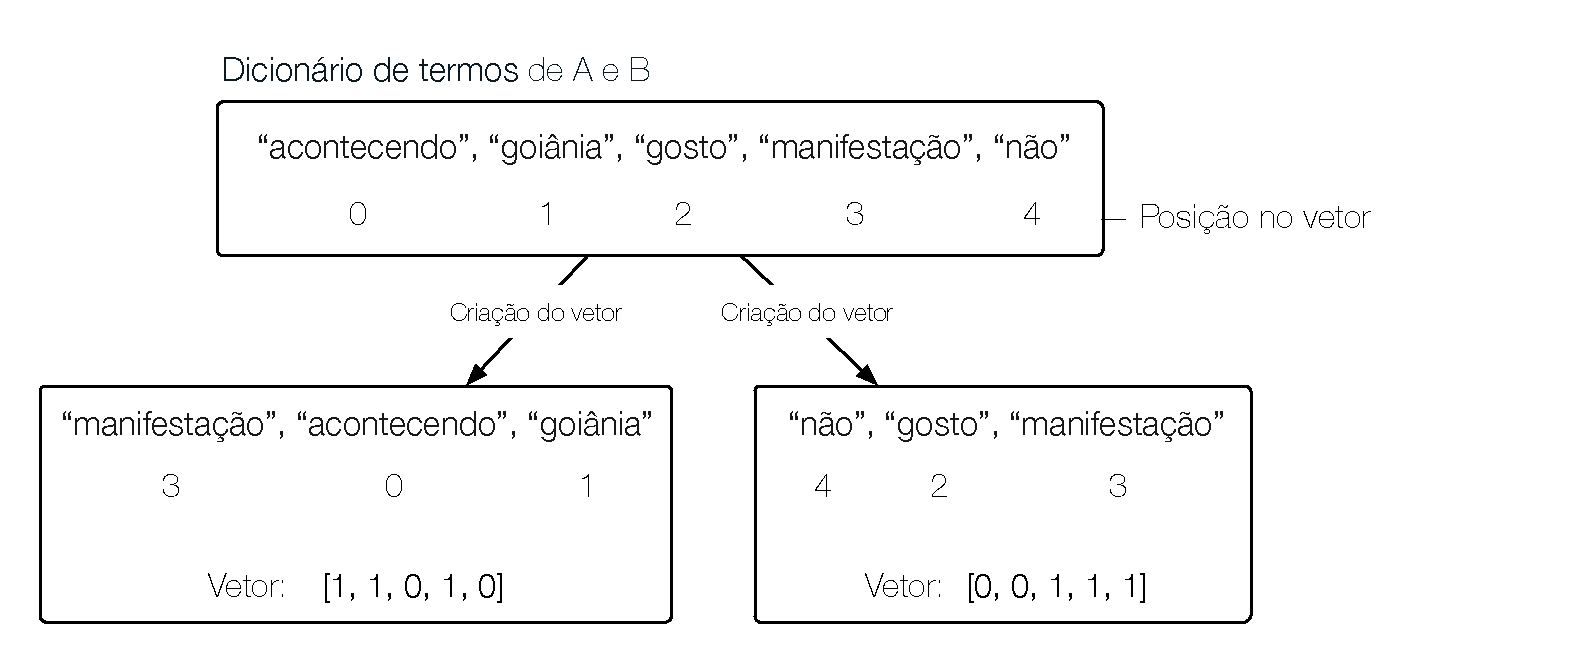
\includegraphics[width=1.0\textwidth]{figuras/vetor-caracteristicas.eps}
		\caption{Criação do modelo de características de duas publicações.}
	\end{center}
\end{figure}

A \textit{Publicação A} é representada pelo vetor [1, 1, 0, 1, 0] - os índices 0, 1 e 3 são marcados como ``1'' pois possuem os termos respectivos no dicionário, e os índices 2, 4 como ``0'' pois não possuem. Similarmente, a \textit{Publicação B} é representada pelo vetor [0, 0, 1, 1, 1].

A conversão dos documentos é necessária para que a classificação das publicações ocorra, pois o classificador não análisa os documentos no formato de texto, e sim na forma de vetores no modelo de espaço vetorial. Cada publicação no modelo de espaço vetorial será um vetor de alta dimensão e muito esparso, ou seja, conterá muitos ``0'', porém a técnica utilizada para classificação posterior é conhecida por ser capaz de lidar com dados com essas características.

\section{Extração dos dados}

A extração e o agrupamento dos dados da publicação, como horário e localização, são relevantes para a sua demonstração no ambiente interativo. Para extrair o \textit{horário} de um evento, o modelo utiliza apenas informação contida na estrutura da publicação. Para extrair a \textit{localização}, são utilizadas três fontes de dados, na ordem: a geolocalização, a cidade na definição do perfil do usuário e a cidade no texto da publicação. 

O dado mais relevante e que é extraído primeiro é a sua \textit{geolocalização}, pois é o que reflete com mais exatidão a localização do evento. Ela consiste na latitude e longitude exata do usuário na hora de criação da publicação. Esse dado é obtido através dos dispositivos GPS presentes em smartphones, tablets e alguns notebooks.

A geolocalização, porém, só está presente em um pequeno número de publicações. Como forma alternativa, o modelo extrai a localização da informação do perfil do usuário. Ao editar o seu perfil, o usuário tem a opção de inserir os dados da sua localização. Esse campo, porém, é livre, e pode conter uma cidade ou não. Para verificar se o campo contém uma cidade, é utilizada uma lista cidades brasileiras. São comparados os termos presentes no campo e na lista e, caso haja a correspondência de algum termo, o modelo considera como uma cidade válida e extrai a localização.

Caso no perfil do usuário não conste cidade alguma, o modelo verifica se o texto da publicação possui uma cidade válida, também de acordo com a lista de cidades. Na Figura 5.2 está apresentada a árvore de decisão para a extração da localização da publicação:

\begin{figure}[htpb]
  \begin{center}
  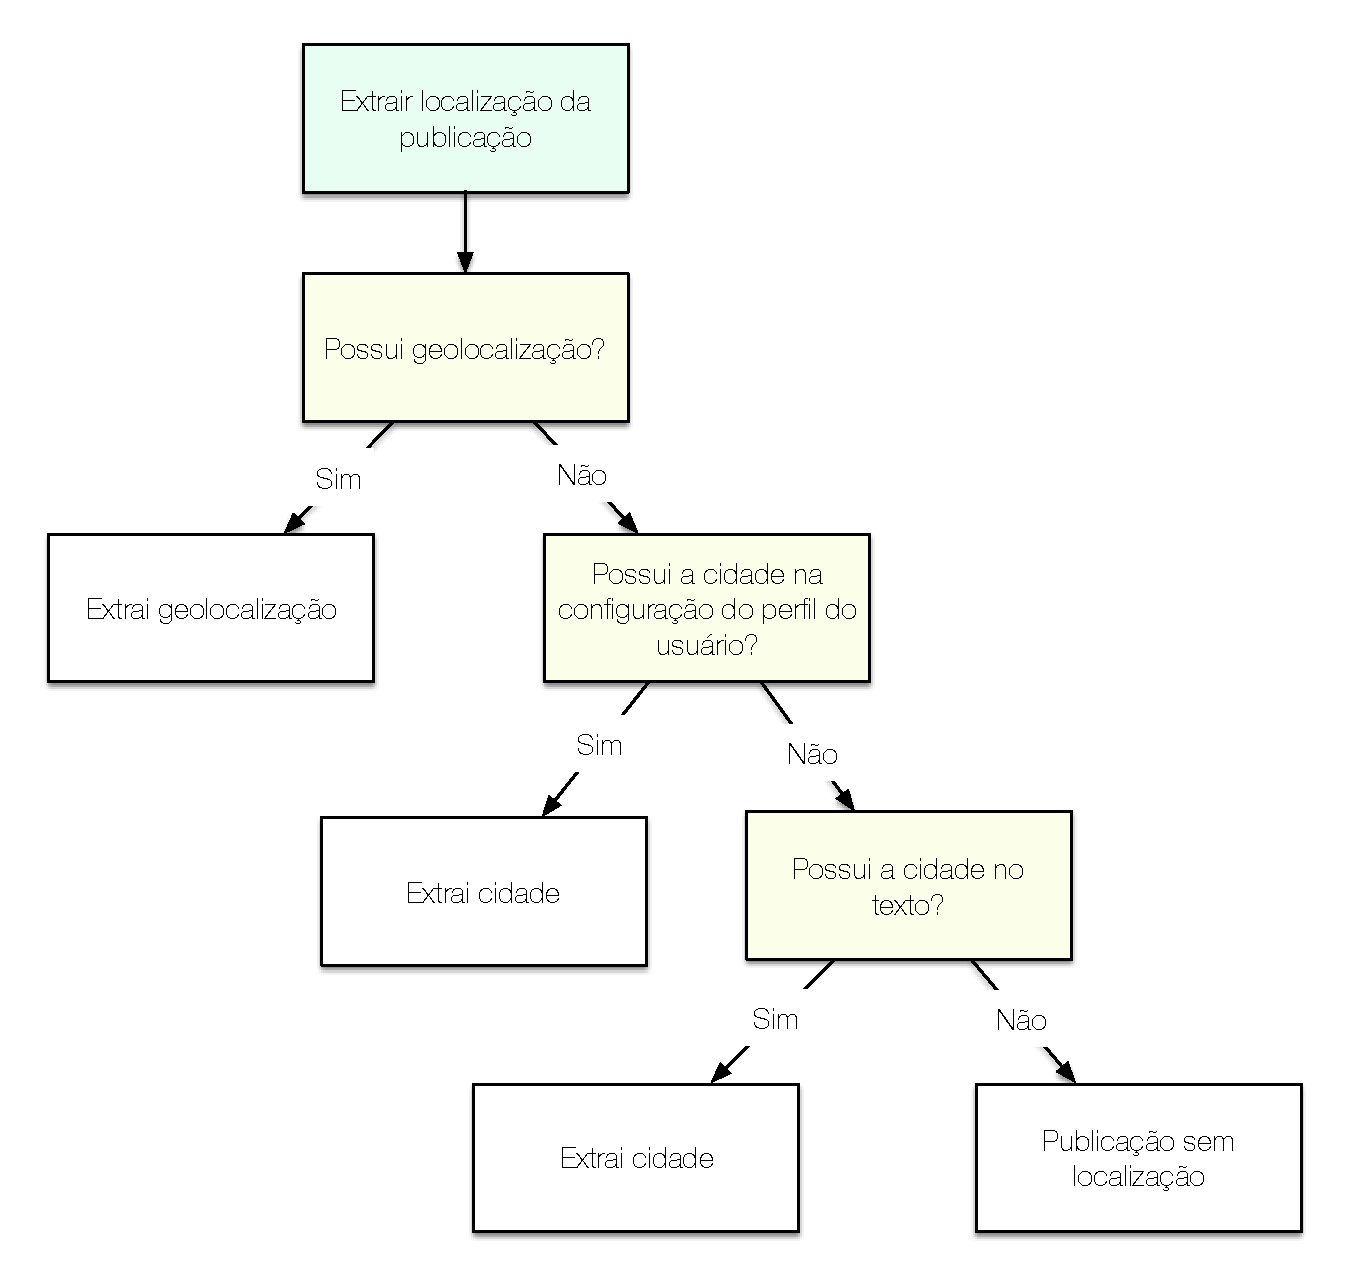
\includegraphics[width=1.0\textwidth]{figuras/extracao-localizacao.eps}
  \caption{Árvore de decisão para extração da localização da publicação.}
  \end{center}
\end{figure}
\chapter{Máquina de aprendizado}

Como no Twitter as publicações criadas por usuários dizem respeito aos mais variados temas, uma busca simples por uma palavra-chave pode retornar publicações relacionadas à ela nos mais variados contextos.

É necessário que o detector de eventos através do Twitter seja capaz de informar se determinada publicação está relacionada ao evento em questão ou não. Essa informação, porém, não pode ser extraída a partir de única publicação. Não é possível, pois, não existem regras para a criação de publicações, e elas podem ser encontradas com as mais variadas combinações e sentidos, portanto não existindo a possibilidade da criação de um conjunto de regras que classifiquem automaticamente as mesmas.

Para resolver esse problema, o modelo implementado utiliza o método de aprendizado supervisionado SVM, para classificar as publicações entre relevantes ou não para a análise.

Os métodos de aprendizado supervisionado são técnicas de aprendizado de máquina que se baseiam na representação do conhecimento do ambiente a partir de um professor. Eles são capazes de aprender as características de um ambiente, ao receberem essa informação de uma fonte externa. Ou seja, o SVM é capaz de receber o conhecimento de quais publicações são relevantes para a análise (dizem respeito à manifestações reais) e quais não são. 

O conhecimento é passado para o algoritmo através da classificação manual de um conjunto de publicacões de amostra. Ao fazer isso, as informações do ambiente estão sendo representadas, o SVM recebe as informações e, através do princípio de indução, consegue utilizar esse conhecimento para fazer induções futuras sobre outros dados.

O SVM possui o conhecimento de cada entrada de informação e baseia-se na semelhança entre os mesmos para determinar as suas classes. Ou seja, ao classificar um conjunto inicial de dados, o que está sendo transferido são os padrões de comportamento pertencente a cada classe. O algoritmo, então, que consegue determinar o comportamento de cada classe e classificar futuros dados baseados nessa semelhança.

O princípio de indução, porém, muitas vezes deve ser sensível à erros de classificação, em casos que o conhecimento total do ambiente não pode ser transferido para o ambiente amostral, devido à quantidade de regras ser infinita ou desconhecida. Em um ambiente hipotético binário, por exemplo, aonde se o dado contém ``X'', a classe é ``1'', e se não contém a classe é ``0'', o algoritmo não precisa ser sensível à erros. Mas ao lidar com documentos de texto, por exemplo, as regras de linguagem são mais complexas do que isso. A quantidade de palavras existentes são muitas e elas podem ser encontradas em ordens diferentes, garantindo que o número de possibilidades sejam infinitas ou impossíveis de serem tratadas. Nesse caso, o algoritmo mesmo que não acerte 100\% das classificações, pode chegar à um número de acertos muito próximo disso, mesmo que as regras não sejam todas definidas. 

Para o modelo implementado, como o total de regras é desconhecido, é necessária um conjunto de publicações que seja relevante para representar o conhecimento ao algoritmo. Se o conjunto for reduzido demais, as regras mais importantes podem não ser representadas e o algoritmo irá falhar ao classificar futuros dados. Porém, se o conjunto for extenso demais, o trabalho em classificá-las manualmente será demasiado. É preciso achar um número de publicações que consiga generalizar os dados e que ainda faça sentido a implementação do algoritmo.

Após a criação dos dados de exemplo, o classificador pode ou não passar pela fase de testes, aonde sua taxa de acertos é analisada e verificada se atende às expectativas. No detector proposto, é criada uma nova base de publicações, que são classificadas manualmente, porém o conhecimento dessa nova base não é transferido para o SVM. O algoritmo é então executado e as saídas são analisadas e comparadas com a classificação manual. Para chegar à um resultado satisfatório, o algoritmo é executado sucessivas vezes. De acordo com a sua taxa de acerto, a base de conhecimento é alterada e o parâmetro de custo do algoritmo é ajustado.

Com o conhecimento devidamente representado, o SVM está apto a classificar futuras ocorrências. O SVM é então executado com a base de publicações obtidas do Twitter, e as ocorrências positivas são utilizadas para serem agrupadas por horário e os eventos serem detectados.

\section{Máquina de vetores de suporte (SVM)}

As \textit{máquinas de vetores de suporte} são um conjunto de métodos desenvolvido por Vladimir Vapnik nos anos 90 que, desde a sua criação, superou em performance muitos outros algoritmos existentes, tornando-os a principal linha de pesquisa na área de aprendizado de máquina nos últimos anos \cite{Grigorik2008}. 

Segundo \citeonline{Joachims1998}, o SVM é adequado para a classificação de texto por possuir proteção contra o ajuste demasiado ao conjunto de dados analisados e utilizar \textit{funções de kernel}, que são capazes de lidar com dados de altíssimas dimensões sem a perda de performance.

O SVM é um \textit{problema de otimização}, que recebe como entrada os vetores de características dos dados e os distribui por uma superfície n-dimensional, para que se possa realizar operações com os mesmos. A Figura 4.1 representa um espaço vetorial de documentos de 3 dimensões.

\begin{figure}[htpb]
	\begin{center}
		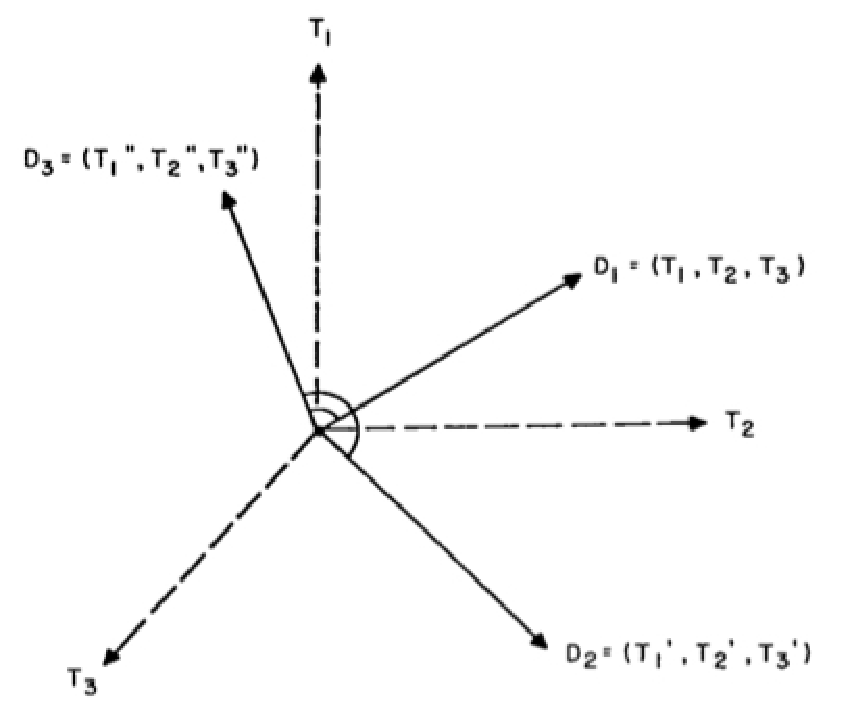
\includegraphics[width=0.6\textwidth]{figuras/representacao-doc.pdf}
		\caption{Representação vetorial do espaço de documentos. \cite{Salton1975}}
	\end{center}
\end{figure}

Para descobrir quais vetores pertencem à quais classes, o SVM tenta achar um plano, de dimensão n-1, que separa os vetores com a maior margem possível. O algoritmo parte do princípio que existe uma diferença fundamental que separa as duas classes e cria a separação espacial entre elas. O método deduz que, após a criação do plano, os vetores de um lado do plano fazem parte de uma classe e os do outro lado de outra classe, o que na prática se mostra funcionar \cite{Grigorik2008}. 

\subsection{Problema de otimização}

Dado o conjunto de $n$ dados de treinamento:

\begin{equation*}
D = \begin{Bmatrix}
({x}_{i}, {y}_{i}) \mid {x}_{i} \in {R}^{d}, {y}_{i} \in \{-1,1\} 
\end{Bmatrix}
\begin{matrix}
n \\ 
i = 1
\end{matrix}
\end{equation*}

aonde cada ponto ${x}_{i}$ é um vetor de características d-dimensional de números reais e ${y}_{i}$ a classe em que o vetor pertence e possui o valor 1 ou -1. Deseja-se encontrar o plano $p$ que divide o os pontos que possuem ${y}_{i} = 1$ dos que possuem ${y}_{i} = -1$. Cada plano pode ser, então, definido em função de $x$.

\begin{equation*}
wx - b = 0,
\end{equation*}

ou de forma simplificada:

\begin{equation*}
{w}^{T}x + b = 0.
\end{equation*}

Sendo ${w}$ o vetor normal do plano $p$ e $b$ o deslocamento em relação a origem. Para ilustrar o SVM, na Figura 4.2 são representados algumas retas possíveis para dividir duas classes de dados no ${R}^{2}$. Para dados no ${R}^{3}$, o divisor dos dados é um plano bidimensional, para dados no ${R}^{n}$, o divisor dos dados é um hiperplano de dimensão $n-1$.

\begin{figure}[htpb]
	\begin{center}
		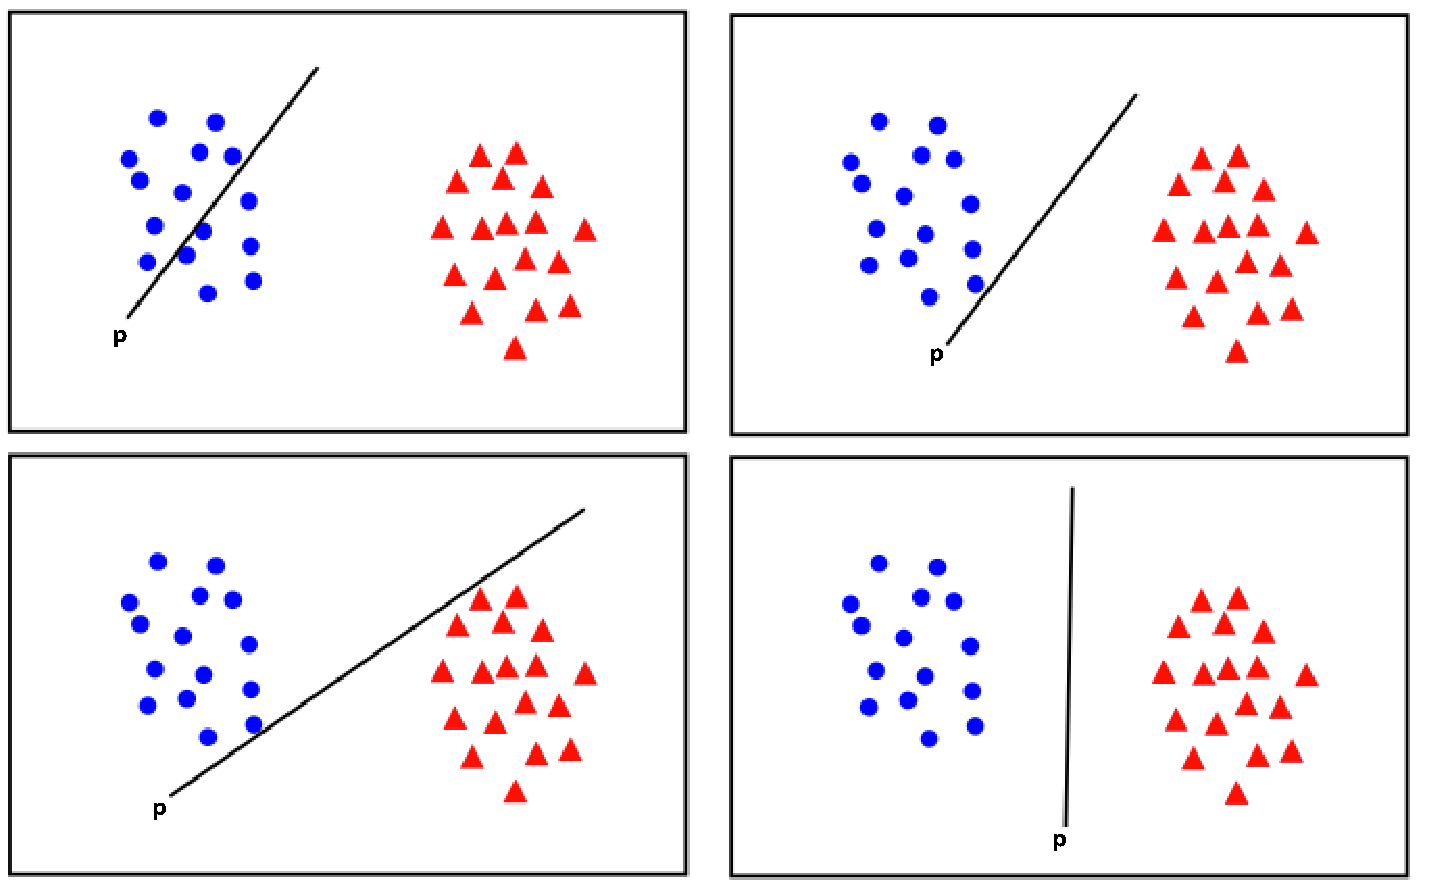
\includegraphics[width=0.6\textwidth]{figuras/svm-plans.pdf}
		\caption{Planos possíveis para divisão de duas classes de dados.}
	\end{center}
\end{figure}

Se os dados de treinamento são linearmente separáveis, é possível encontrar dois planos que os separam sem existir nenhum ponto entre eles. Como ${y}_{i}$ possui valor 1 ou -1, os planos que se encontram exatamente no limiar dos pontos são definidos pelas equações (como ilustrado na Figura 4.3):

\begin{equation*}
{w}^{T}x + b = 1,
\end{equation*}

e

\begin{equation*}
{w}^{T}x + b = -1.
\end{equation*}

\begin{figure}[htpb]
	\begin{center}
		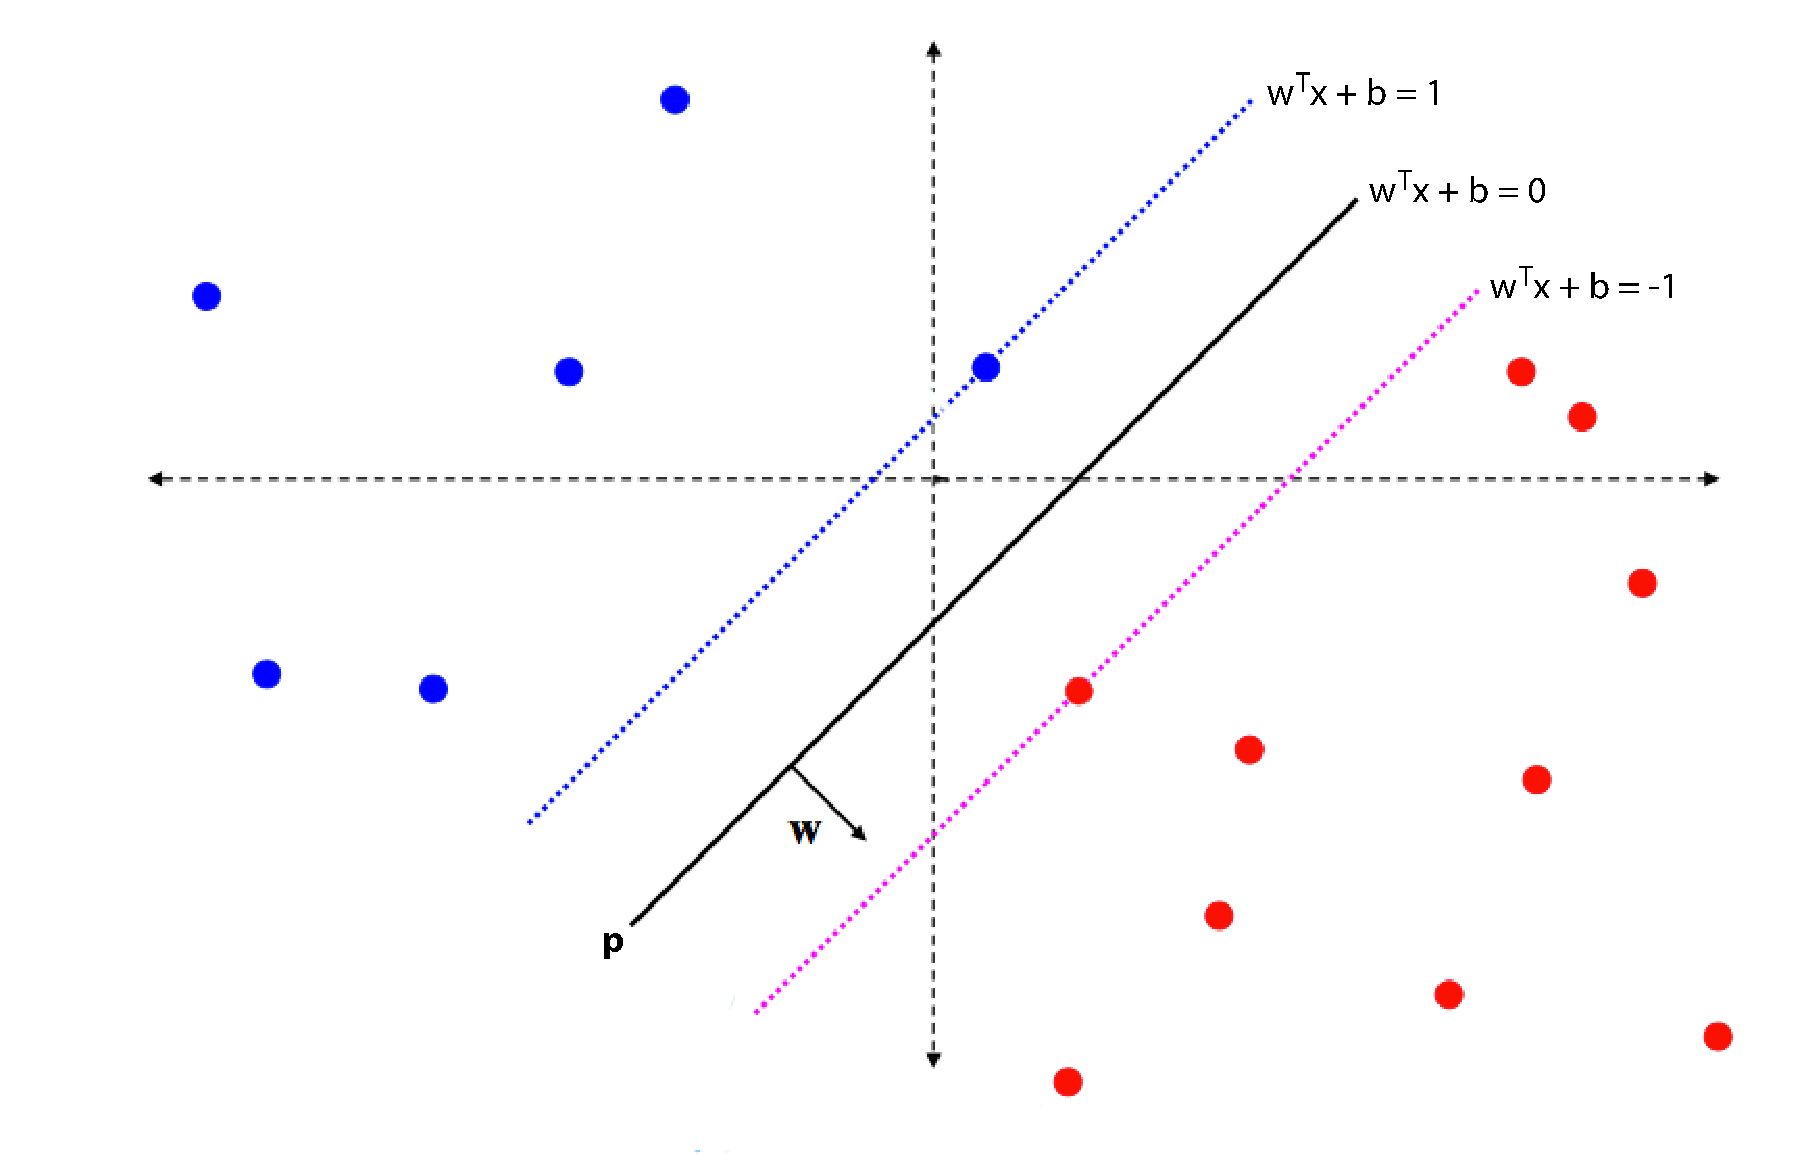
\includegraphics[width=0.8\textwidth]{figuras/svm-plans-2.pdf}
		\caption{Planos no limiar dos pontos.}
	\end{center}
\end{figure}

Ou seja, a função de classificação pode ser definida como:

\begin{equation*}
  \begin{cases}
	{w}^{T}x + b \geq 1 & \text{ para ${x}_{i}$ da primeira classe }  \\ 
	{w}^{T}x + b \leq -1 & \text{ para ${x}_{i}$ da segunda classe }
	\end{cases}
\end{equation*} 
	
Na forma reduzida:

\begin{equation*}
	{y}_{i}({w}^{T}{x}_{i} + b) \geq 1, \text{para todo } 1 \leq i \leq n
\end{equation*}

Somente os pontos mais próximos, chamados de \textit{vetores de suporte}, influenciam a criação dos planos, ao contrário do filtro de kalman e regressão linear, por exemplo, que utilizam todos os pontos para gerar o modelo. A distância entre os vetores de suporte positivos e negativos delimita a \textit{margem}.

Para calcular a margem, como ${w}^{T}x + b = 0$ e $c({w}^{T}x + b) = 0$ definem o mesmo plano, é possível escolher a normalização de $w$. A normalização é escolhida tal que ${w}^{T}{x}_{+} + b = 1$ e ${w}^{T}{x}_{-} + b = -1$, para os vetores de suporte positivos e negativos. A margem entre os planos pode ser escrita, então, por:

\begin{equation*}
	\frac{w}{||w||}({x}_{+} - {x}_{-}) = \frac{{w}^{t}({x}_{+} - {x}_{-})}{||w||} = \frac{2}{||w||}
\end{equation*}

O problema de otimização do SVM é maximizar a margem $\frac{2}{||w||}$, ou seja, minimizar $||w||$ (como ilustrado na Figura 4.4). Podendo ser descrito, então, como:

\begin{equation*}
\begin{matrix}
\min & ||w|| & \\ 
\text{sujeito à } & {y}_{i}({w}^{T}{x}_{i} + b) \geq 1, & \text{para todo } 1 \leq i \leq n
\end{matrix}
\end{equation*}

\begin{figure}[htpb]
	\begin{center}
		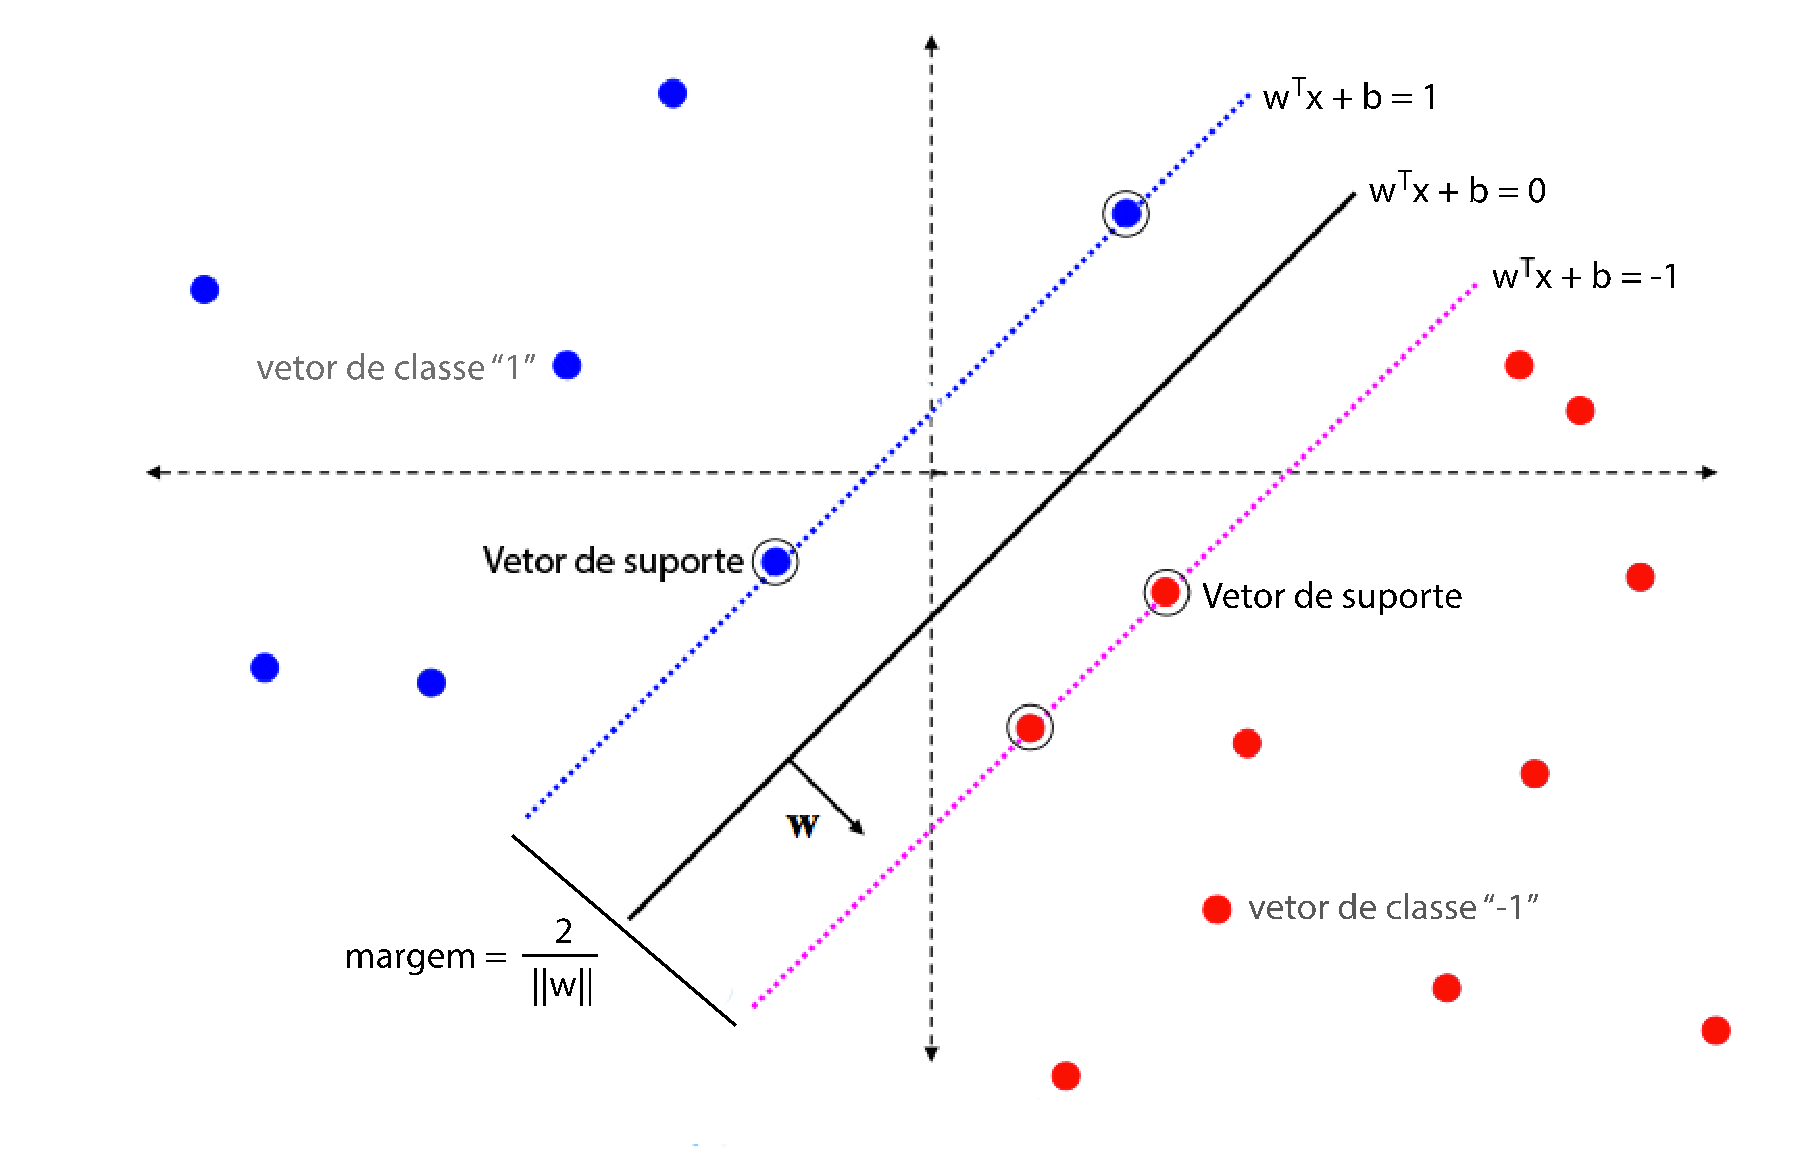
\includegraphics[width=0.7\textwidth]{figuras/svm-regions-2.pdf}
		\caption{Margem entre os planos.}
	\end{center}
\end{figure}

Nesse método, chamado de \textit{SVM de Margem Rígida}, o modelo se enquadra exatamente aos dados de exemplo. Mas podem existir casos aonde os dados são linearmente separáveis, porém existe uma margem muito pequena entre os vetores de suporte. Nesse caso, o exemplo tentará dividir as classes encontrando como plano ideal um de margem muito pequena, mas talvez um plano de margem maior e que ignore certos pontos seja uma solução mais satisfatória, como ilustrado na Figura 4.5.

\begin{figure}[htpb]
	\begin{center}
		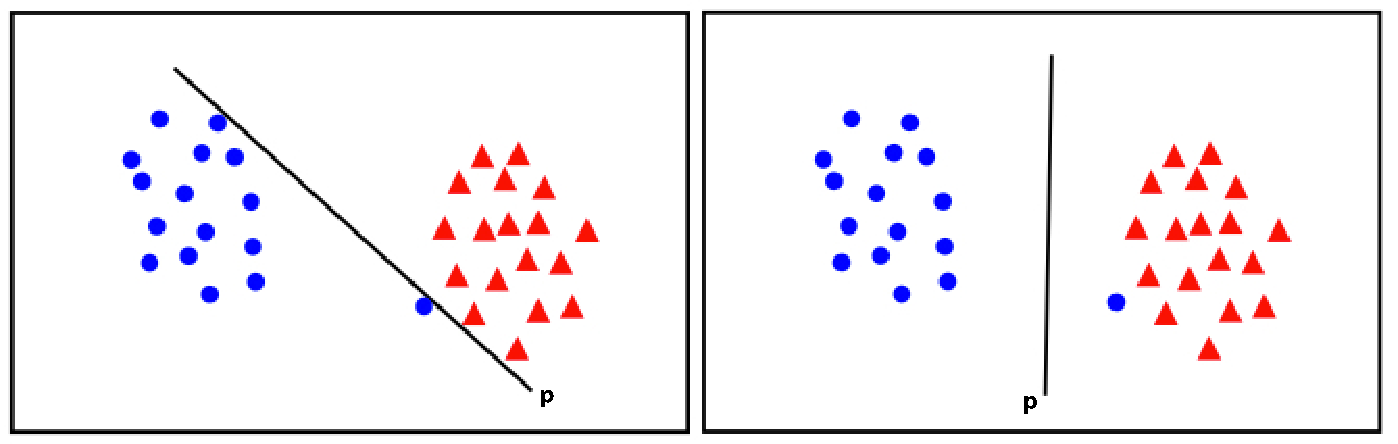
\includegraphics[width=0.7\textwidth]{figuras/svm-soft-margin.pdf}
		\caption{Plano de maior margem que ignorando certos pontos.}
	\end{center}
\end{figure}

O método SVM que permite erros de classificação é chamado de SVM de Margem Suave (\textit{Soft Margin SVM}).

\subsection*{SVM de Margem Suave}

O método Margem Suave introduz a variável de folga ($\xi$):

\begin{equation}
\begin{matrix}
\min & ||w|| + C \sum {\xi}_{i} & \\ 
\text{sujeito à } & {y}_{i}({w}^{T}{x}_{i} + b) \geq 1 - {\xi}_{i}, & \text{para todo } 1 \leq i \leq n
\end{matrix}
\end{equation}

\begin{itemize}
	\item Se $\xi = 0$, o ponto está na margem ou após
	\item Se $0 < \xi \leq 1$, o ponto está entre a margem e o lado correto (violação de margem)
	\item Se $\xi \geq 1$, o ponto está do lado errado, como indicado na Figura 4.6.
\end{itemize}

\begin{figure}[htpb]
	\begin{center}
		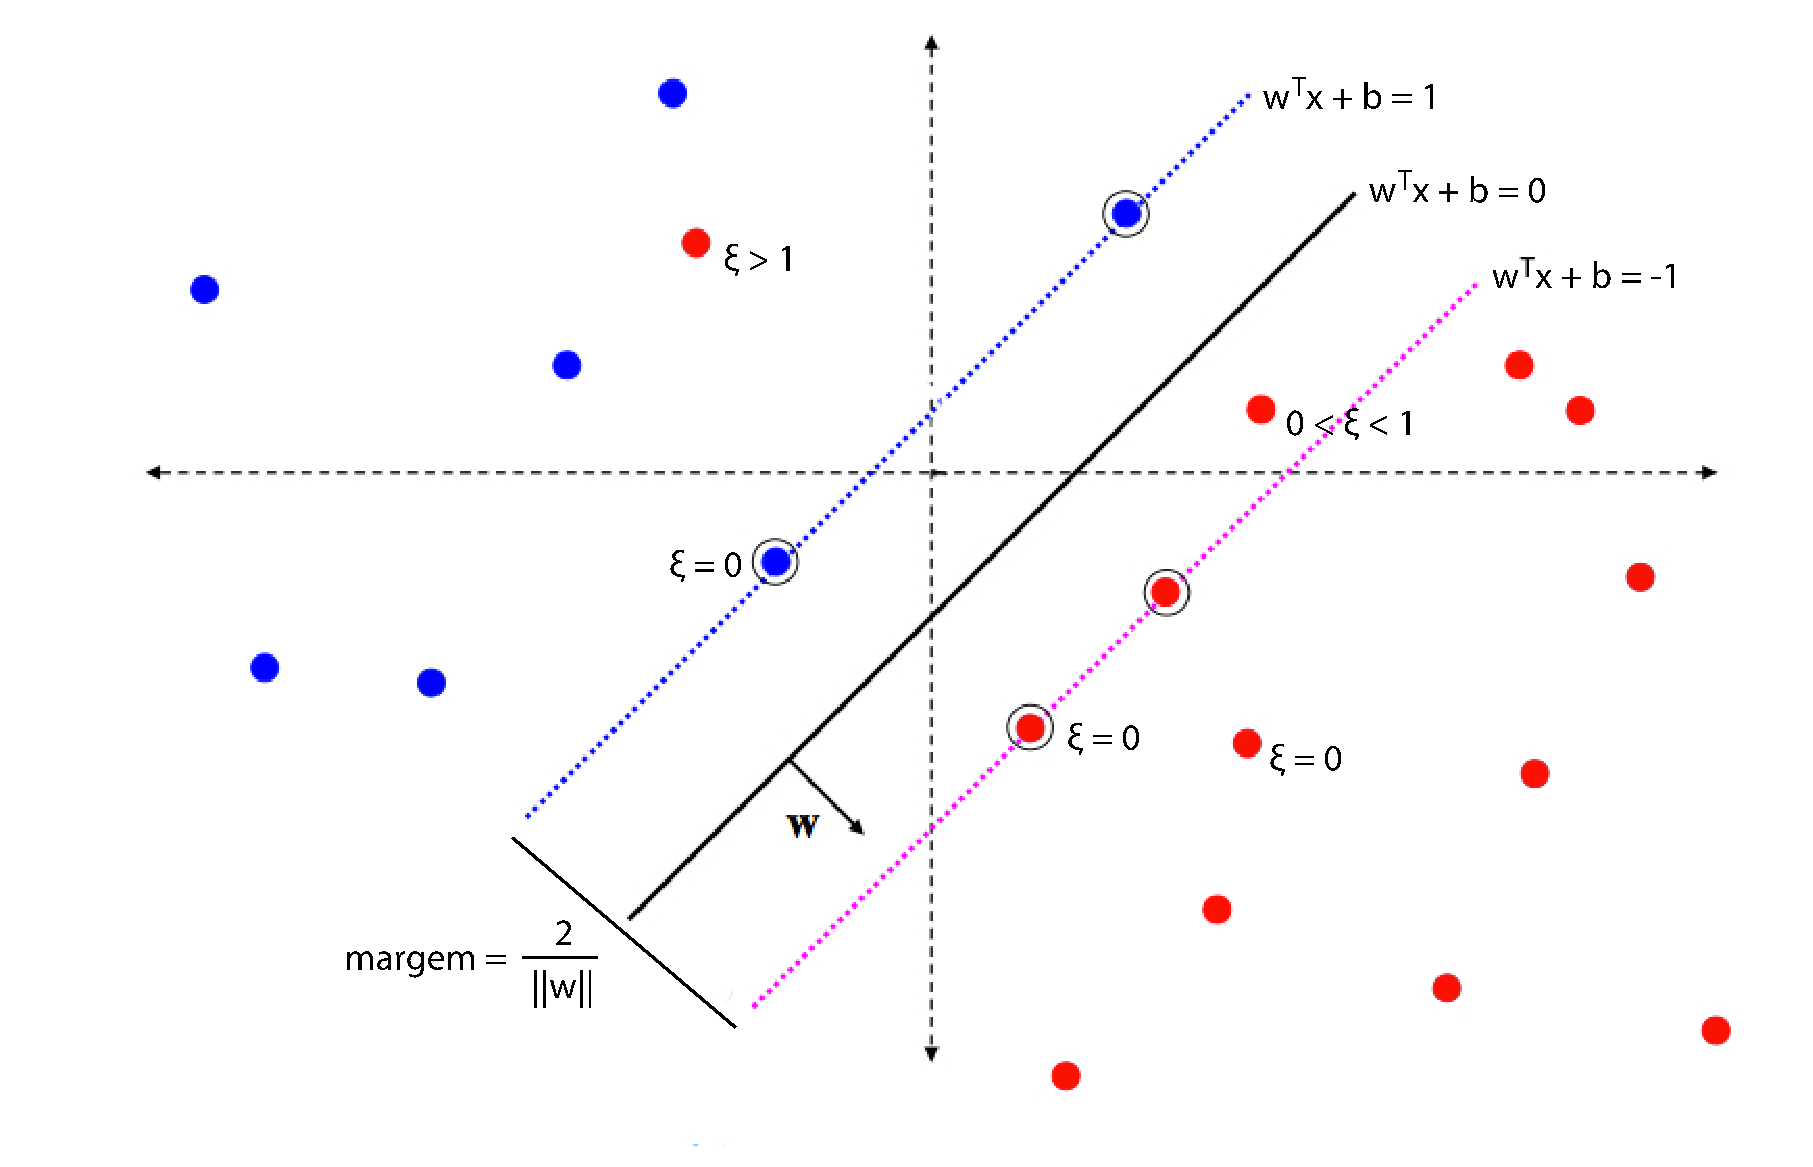
\includegraphics[width=0.8\textwidth]{figuras/svm-epsilons.pdf}
		\caption{Valores para $\xi$.}
	\end{center}
\end{figure}

O algoritmo inclui também a constante de custo ($C$), que representa qual o custo de cada erro de classificação e deve ajustado de acordo com o conjunto de dados de exemplo através de validação. 

\begin{itemize}
	\item Se o valor de $C$ é baixo, as restrições são ignoradas facilmente: maior margem.
	\item Se o valor de $C$ é alto, as restrições são mais difíceis de ser ignoradas: menor margem.
	\item Se $C = \propto$, nenhuma restrição é ignorada: \textit{Margem Rígida}.
\end{itemize}

O ajuste correto de $C$ é importante pois aumenta ou diminui a performance do classificador referente ao conjunto de dados da representação de conhecimento. É preciso achar um valor para $C$ que reflita a base de exemplos, para maximizar os acertos do classificador. Se a representação de conhecimento está bem generalizada, é possível que se possa escolher um valor alto para $C$, pois os erros esperados serão poucos. Se está mal generalizada, talvez $C$ com um baixo seja mais adequado, pois espera-se mais erros e mais versatilidade por conta do classificador.

É possível que, mesmo com margem suave, o SVM não consiga classificar os dados de forma linear. Caso isso ocorra, e necessária a aplicação de \textit{funções de kernel}, que são funções que aplicam transformações nos dados para que sejam mais facilmente classificáveis.

\subsection*{Funções de Kernel}

As \textit{funções de kernel} são uma classe de algoritmos utilizados para encontrar e estudar tipos de relações em conjuntos de dados. Atualmente, elas tem recebido grande atenção, particularmente devido à popularidade do SVM. Como pode ser observado nos trabalhos de \citeonline{Ali2005}, \citeonline{Ozer2013}, \citeonline{Megri2014}, entre outros.

As funções de kernel mapeam os dados em um espaço de maior dimensão, com o intuito de que esse espaço seja mais facilmente classificado. A Figura 4.8 representa um espaço de duas dimensões mapeados para um espaço de três dimensões.

\begin{figure}[htpb]
	\begin{center}
		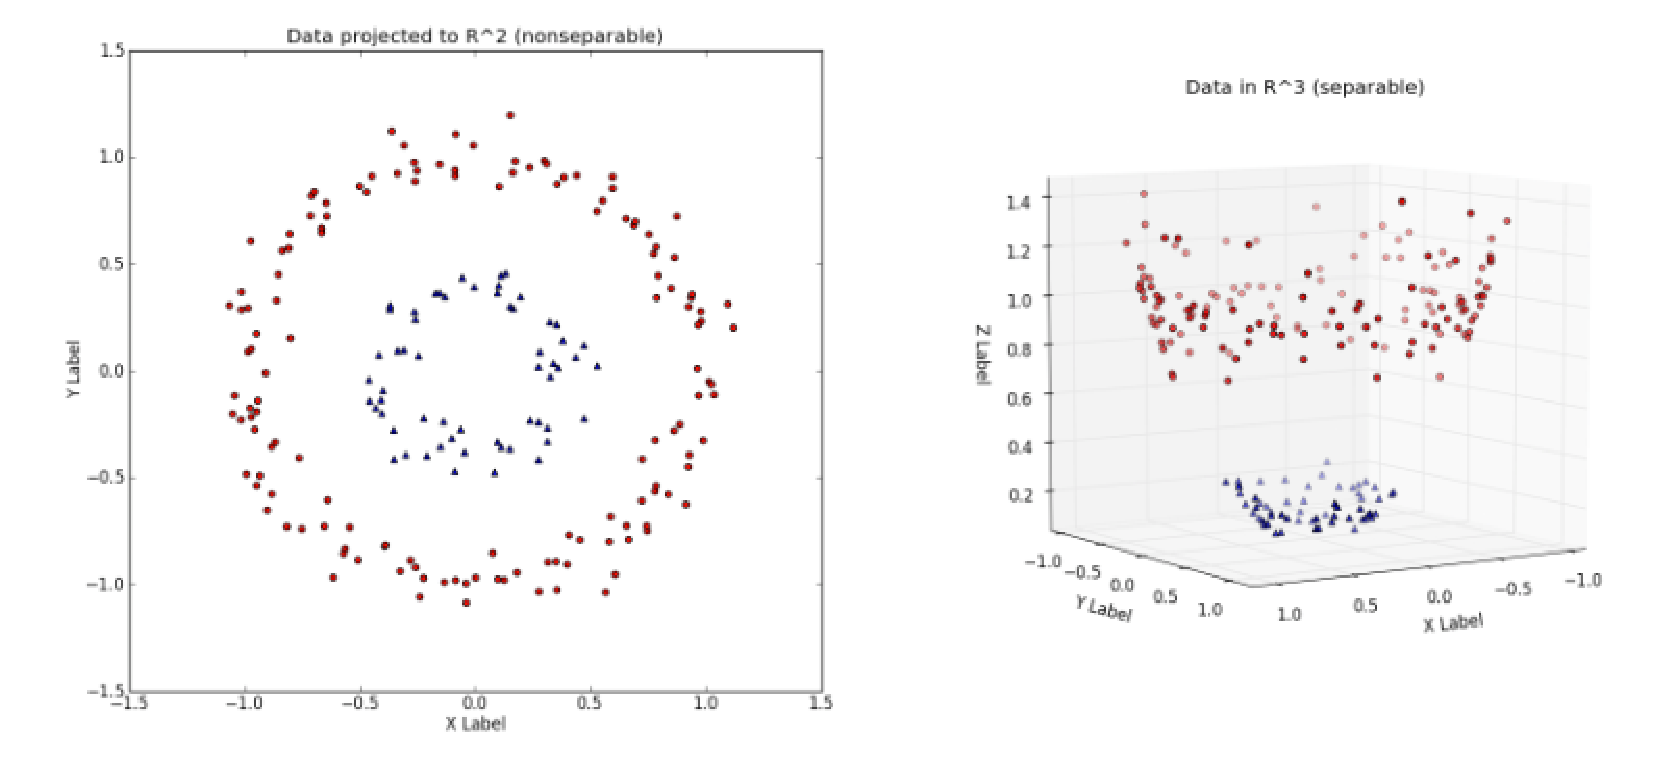
\includegraphics[width=0.9\textwidth]{figuras/svm-kernel.eps}
		\caption{Um conjunto de dados no ${R}^{2}$ (não separáveis) transormados para ${R}^{3}$ (separáveis) pela função de kernel $[{x}_{1}, {x}_{2}] = [{x}_{1}, {x}_{2}, {x_1}^{2} + {x_2}^{2}]$ \cite{Kim2013}.}
	\end{center}
\end{figure}

Os kernels são utilizados em problemas que não precisam operar com os vetores no espaço de maior dimensão, como é o caso do SVM. As funções calculam o produto escalar dos dois vetores no espaço de maior dimensão, sem explicitamente transformá-los para esse espaço. Esse fato possibilita que os kernels operem em dados sem calcularem suas coordenadas, podendo operar em espaços de qualquer dimensão (infinitas) e implícitos.

Existe uma grande variedade de kernels disponíveis. Segundo \citeonline{Grigorik2008}, o \textit{kernel linear} é geralmente bom para 99\% dos casos, mas a escolha da função de kernel adequada pode melhorar a performance do classificador.

\section{Representação do conhecimento}

O SVM é um classificador de aprendizado supervisionado, ou seja, é capaz de aprender à dividir um conjunto de dados em classes distintas. O método aprende a realizar a classificação através da \textit{representação do conhecimento} desse conjunto de dados.

Na representação do conhecimento, algumas ou todas características do conjunto de dados são previamente transferidas para o classificador. Esse conhecimento é transferido pela figura de um professor, que as informa ao classificador com o intuito que ele possa fazer induções futuras a partir dessas informações.

A fase em que se informa propriamente conhecimento ao classificador é denominada de \textit{treinamento}, aonde serão passados tipicamente os vetores de características ${x_i}$ de dados de exemplo e suas respectivas classes ${y_i}$ ao SVM.

Após a fase de treinamento, o SVM pode passar, ou não, pela fase de testes. Aonde o classificador é executado para testar se suas saídas estão satisfatórias, se sua taxa de acerto é aceitável para o modelo em questão. Nesse caso, os vetores de características ${x_i}$ são inseridos, porém as suas classes ${y_i}$ são obtidas pelas saídas do SVM.

\subsection{Treinamento}

Para o treinamento do SVM, o conjunto de dados para ${x_i}$ e ${y_i}$ é criado. Para o modelo implementado, ${x_i}$ serão os vetores de características das publicações, e ${y_i}$ as suas respectivas classes. Cada classe de publicação ${y_i}$ possuirá valor ``1'' caso seja uma ocorrência real de manifestação e ``-1'' caso não seja. Como indicado na Figura 4.9. 

\begin{figure}[htpb]
	\begin{center}
		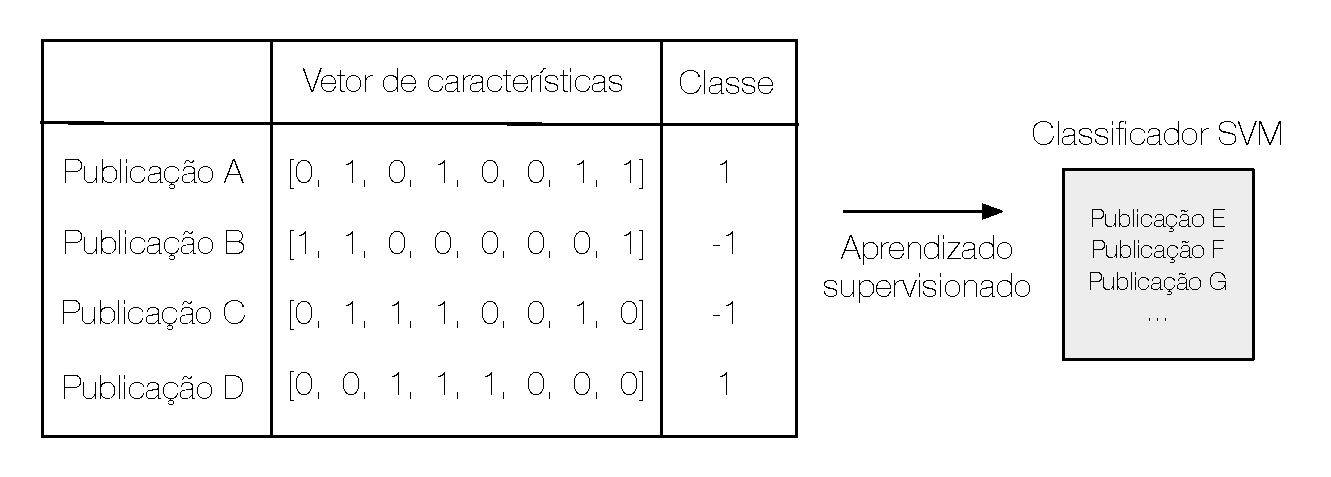
\includegraphics[width=0.8\textwidth]{figuras/inducao-aprendizado-supervisionado.eps}
		\caption{Treino do SVM.}
	\end{center}
\end{figure}

As publicações que indicam a ocorrência de um evento de manifestação podem se apresentar de várias formas, mas devem possuir pelo menos uma característica: representam uma manifestação real, com local e horário, que ocorre no momento da publicação.

As publicações negativas também se apresentam de várias maneiras, não importando muito suas características, podendo ser publicações que mencionam uma manifestação que já aconteceu, que citam uma manifestação que acontecerá no futuro, que utilizam a palavra-chave em outro contexto, etc. 

Um exemplo de publicação positiva é a frase ``manifestação agora na rua Rio Branco'', que informa corretamente o acontecimento de um evento de manifestação e o seu local. Um exemplo negativo é a frase ``odeio manifestação'', que apenas menciona a palavra, não se referindo à um evento. A Tabela 3 apresenta alguns outros exemplos.

\begin{table}[ht]
	\caption{Publicações de treino.}
	\centering
	\begin{tabular}{| p{7cm} | p{7cm} |}
		\hline
		\textbf{Positiva (1)} & \textbf{Negativa (-1)} \\ [0.5ex] \hline \hline
    ``manifestação agora na rua Rio Branco.'' & ``odeio manifestação'' \\ \hline
    ``grupo bloqueia avenidas de SP em manifestação'' & ``vamos fazer uma manifestação'' \\ \hline
    ``ativias param rua de BH em manifestação'' & ``ontem teve manifestação aqui na minha cidade'' \\ \hline
    ``MANIFESTAÇÃO: estudantes bloqueiam BR-101'' & ``sabe se está tendo manifestação?'' \\
    ... & ... \\ [1ex]
		\hline
	\end{tabular}
	\label{table:nonlin}
\end{table}

Para representar esse conhecimento ao SVM, uma base de publicações, as \textit{publicações de treino}, é selecionada a partir do total de publicações obtidas pelo Twitter para o mês de Agosto. As publicações de treino são lidas e classificadas manualmente. Espera-se, então, que ao alimentar o SVM com esse conhecimento, o método consiga aprender os padrões pertencentes à cada classe de publicação e consiga induzir as classes de ocorrências futuras.

Com ${x_i}$ e ${y_i}$ conhecidos, o problema de otimização da Equação 4.1 pode ser resolvido de diversas maneiras, uma delas sendo a \textit{programação quadrática}. O método encontra $w$ e $b$, a partir dos $n$ dados conhecidos de $x$ e $y$. Nesse caso, as publicações de treino e suas respectivas classes.

Com $w$ e $b$ encontrados, o SVM pode ser testado e visto se com os $x$ e $y$ informados, foi suficiente para que ele possa realizar classificações futuras com uma taxa de acerto aceitável.

\subsection{Teste}

Para determinar se a representação do conhecimento é suficiente para o SVM classificar futuras ocorrências, ele é testado em um conjunto de \textit{publicações de teste}. Cada publicação é classificada manualmente, porém a informação não é inserida no classificador. O SVM é então executado e as classificações geradas são comparadas com as classificações manuais.

Como $w$ e $b$ já são conhecidos, a classe $y_i$ do vetor de características $x_i$ de cada publicação pode ser determinada pela seguinte expressão:

\begin{equation}
{y}_{i} = {w}^{T}{x}_{i} + b
\end{equation}

Caso $w$ e $b$ foram gerados satisfatoriamente na fase de treino, as saídas para $y_i$ serão, na maioria das vezes, as classes corretas das publicações.

Caso o classificador não apresente resultados satisfatórios, é possível que o conhecimento não esteja devidamente representado na base de treino e $w$ e $b$ estejam com valores divergentes, ou ainda que o parâmetro $C$ esteja mal ajustado.

A mudança mais fácil de ser feita, nesses casos, é o ajuste do parâmetro $C$. O mesmo deve ser ajustado de acordo com a a base de conhecimento. Se a base estiver bem generalizada, é possível escolher um valor para $C$ mais alto, pois espera-se que o classificador erre pouco. Caso a base não esteja bem generalizada, talvez seja mais adequado escolher $C$ mais baixo, pois ele irá permitir mais versatilidade de adequamento aos dados, porém também permitirá que mais erros ocorram. 

No modelo implementado, o parâmetros $C$ é ajustado através de sucessivos testes, de acordo com a taxa de acerto do classificador. Para implementações com mais parâmetros ou que não seja possível o ajuste manual de $C$, talvez seja necessário a utilização de ferramentas que otimizam múltiplos parâmetros de forma automatizada, como proposto por \citeonline{Chapelle2002}.

Caso o seu ajuste não impacte em mudanças nos acertos das classificações, é possível que o conhecimento não esteja devidamente representado. Se a base de treino for insuficiente, é possível que esteja com poucos exemplos das possibilidades do ambiente ou com exemplos que não reflitam essas possibilidades. O primeiro caso resolve-se inserindo mais exemplos na base. O segundo, troncando os exemplos pelos que melhor representam o ambiente.

Após os devidos ajustes, o SVM precisa ser executado novamente e as saídas novamente comparadas. Para tornar os testes viáveis, o conjunto de dados de teste precisa ser enxuto o suficiente para ser comparado manualmente, porém não muito reduzido para ainda ser relevante. 
\chapter{Modelo implementado e resultados}

O modelo implementado implementa todo o processo através de classes nativas da linguagem Ruby\footnote{http://ruby-lang.org} e de interfaces de comunicação com outros serviços como a Search API do Twitter e a biblioteca LIBSVM.

Para a obtenção das publicações, é utilizada a interface da \textit{Search API} do Twitter para a linguagem. A interface realiza a ponte entre as chamadas HTTP necessárias para a API do Twitter em classes Ruby. Através da interface, são chamados métodos que buscam a palavra-chave ou expressão desejada, entre as datas especificadas. No caso do modelo, a palavra-chave ``manifestação'', entre 01 e 31 de Agosto de 2014. A Search API, porém, não retorna publicações com mais de uma semana de criação\footnote{A interface \textit{Search API} possui a restrição de busca de publicações para apenas uma semana depois da sua criação.}, foi preciso, então, realizar mais de uma busca, em datas diferentes. 

As publicações obtidas são salvas localmente em um arquivo CSV, e posteriormente são separadas em mais dois arquivos, um para a fase de testes e outro para a fase de treino. Para manipular os arquivos, é utilizada a biblioteca \textit{CSV} nativa do Ruby, que permite que sejam criados novos arquivos e carregadas suas informações.

A conversão para o modelo de espaço vetorial é feita utilizando classes para manipulação de cadeias de caracteres (\textit{String}) e vetores (\textit{Array}) do Ruby. Através de métodos dessas classes, é possível aplicar todos os passos da conversão, como: tokenização, pré-processamento, criação do dicionário de termos e conversão para vetores de características.

Com os vetores de características obtidos, a classificação das publicações com SVM é feita utilizando a interface Ruby para biblioteca LIBSVM\footnote{http://www.csie.ntu.edu.tw/~cjlin/libsvm/}. A biblioteca LIBSVM implementa diferentes formulações de máquina de vetores de suporte (SVM) e funções de kernel. A interface para Ruby permite que a biblioteca seja utilizada através de classes da linguagem e que a classificação seja aplicada de forma integrada com o resto do processo.

Após a classificação, é feita a extração dos dados do horário e localização. O horário é extraído diretamente a partir da informação presente no arquivo CSV. A localização, é extraída de acordo com qual dado será utilizado: caso a geolocalização esteja presente, esse dado é diretamente retirado do arquivo. Caso não esteja, é utilizada a informação obtida no processo de tokenização da publicação para identificar se, nos termos presentes, está contida alguma cidade brasileira. Caso no texto não esteja, é aplicada a tokenização na informação do perfil do usuário e realizado o mesmo processo de identificação.

Para a criação do ambiente, foi utilizada a ferramenta para desenvolvimento de aplicações web Ruby on Rails\footnote{http://rubyonrails.org}. No ambiente são exibidos gráficos de série-temporal das publicacões, divididas primeiramente por dias e posteriormente por horas. É possível visualizar cada faixa de horário da publicação em um mapa de marcadores, em que as publicações são agrupadas de acordo com a sua localização, o que permite a visualização do horário e da localização dos eventos. 

O código completo implementado que obtem as publicações, as converte para o modelo de espaço vetorial e a as classifica com SVM, se encontra no Apêndice A. Aqui serão apresentadas apenas as partes mais relevantes do código, de acordo com a organização das seções dos capítulos anteriores.

\section{Obtenção de publicações via Search API}

Para obter as publicações é utilizada a Search API do Twitter, na sua versão 1.1. É utilizada uma interface Ruby para a API, que cria classes para lidar com as chamadas HTTP. Ao invés de lidar com o código referente a requisições HTTP, o que dificulta a sua implementação e legibilidade do código, é possivel lidar direto com métodos de classes Ruby. 

A interface possui o mesmo nome do serviço e o modelo utiliza a sua versão 5.8.0. Para instalar a interface, utitilizamos o gerenciador de extensões do Ruby Rubygems\footnote{https://rubygems.org}. Após a instalação do gerenciador, ela é instalada rodando o código a partir do terminal:

\begin{lstlisting}
  gem install twitter --version 5.8.0
\end{lstlisting}

Com a interface instalada, para realizar chamadas à Search API do Twitter, é preciso cadastrar um \textit{aplicativo} no serviço\footnote{https://apps.twitter.com} e configurar as chaves que são recebidas. São recebidas 4 chaves: uma chave da API (\textit{consumer key}), um código secreto da API (\textit{consumer secret}), um token de acesso do aplicativo (\textit{access token}) e um código secreto do aplicativo (\textit{access token secret}):

\begin{lstlisting}
  class Twitter
    def initialize
      @cliente = Twitter::REST::Client.new do |config|
        config.consumer_key        = "DbT8fYWR2jq1TIXvxVtiZzFno"
        config.consumer_secret     = "3mT9JcwgaWs5gT...tnAWufYMVyUmle"
        config.access_token        = "42659961-4wDJC...gBaE26GpI5kjC3CK"
        config.access_token_secret = "OjhVszJ3Dyivaz...inoaFiWK7FjY"
      end
    end
  end
\end{lstlisting}

Para a configuração no ambiente, é criada a classe Twitter e inicializada a variável para o \textit{@cliente}. A variável recebe uma instância da classe da interface \textit{Twitter::REST::Client}\footnote{em Ruby, ``::'' significa que o termo seguinte é um módulo (ou classe) do anterior} que recebe as chaves criadas em seus respectivos atributos.

Após a configuração das chaves, é possível realizar as chamadas à API. As chamadas são feitas pelo método \textit{Client\#search}\footnote{em Ruby, ``\#'' significa que o termo seguinte é um método de instância do termo anterior}, que recebe como parâmetro a palavra-chave ou expressão à ser buscada e uma instância da classe \textit{Hash} contendo diversas chaves como linguagem, o identificador máximo e mínimo da publicação (retorna apenas publicações com o identificador maior do que o especificado), o limite de publicações a serem retornadas, etc:

\begin{lstlisting}
  publicacoes = @cliente.search("manifestação", lang: "pt", max_id: "200", since_id: "100", count: 100)
\end{lstlisting}

A Search API, porém, exibe duas restrições de busca:

\begin{itemize}
  \item \textbf{Quantidade:} Retorna apenas um número reduzido de publicações por vez.
  \item \textbf{Tempo:} Não retorna publicações mais antigas do que uma semana.
\end{itemize}

Para obter as publicacões em um período de um mês através da Search API, é preciso contornar essas restrições. Para contornar a restrição de quantidade, são criados ciclos de buscas. Para contornar a restrição de tempo, são executados os ciclos em diversas datas diferentes, respeitando os limites de uma semana.

Para determinar o momento de parar o ciclo de buscas, é definida uma data e passada como primeiro parâmetro para o método \textit{Twitter\#buscar}. O segundo parâmetro determina a expressão a ser buscada, e o terceiro o caminho do arquivo CSV que as publicações serão salvas. 

Para cada chamada ao método \textit{Twitter\#buscar}, é executado um ciclo de buscas, tal como mostra as linhas 6 a 10 do código a seguir. Para cada busca, a última publicação retornada tem o seu identificador armazenado, que é passado para a próxima busca, para ser utilizado como o parâmetro \textit{max\_id}. Assim, a cada busca subsequente, apenas as publicações a partir daquele identificador específico são retornadas. Além do \textit{id}, a data da última publicação retornada também é armazenada e, caso seja menor que a passada como parâmetro o ciclo para. O código a seguir representa o primeiro ciclo de buscas:

\begin{lstlisting}
  class Twitter
    def buscar data_limite, expressao, caminho_arquivo
      data_publicacao = Time.now
      id_maximo = nil

      while publication_date > data_limite
        publicacaoes = @cliente.search(expressao, lang: "pt", max_id: id_maximo).to_a
        data_publicacao = publicacaoes.last.created_at
        id_maximo = publicacoes.last[:id] - 1
        (...)
      end
    end
  end
  twitter = Twitter.new
  data_limite = Time.new(2014, 8, 28, 0, 0, 0, "-03:00")
  twitter.buscar data_limite, "manifestação", "publicacoes_0108_0708.csv"
\end{lstlisting}

Para as seguintes datas de busca, a \textit{data\_limite} e o caminho do arquivo (linha 15 e 16 do código anterior) são modificados para que a busca retorne apenas as publicações criadas após a data em que a última busca foi feita, como indicado pelo código a seguir:

\begin{lstlisting}
  data_limite = Time.new(2014, 08, 1, 0, 0, 0, "-03:00")  # No dia 01/08
  twitter.buscar data_limite, "manifestação", "publicacoes_0108_0708.csv"
  data_limite = Time.new(2014, 08, 7, 0, 0, 0, "-03:00") # No dia 07/08
  twitter.buscar data_limite, "manifestação", "publicacoes_0808_1408.csv"
\end{lstlisting}

Para manipular arquivos CSV e salvar as publicações a cada busca, é utilizada a biblioteca do Ruby \textit{CSV}. Para abrir o arquivo é utilizado o método \textit{CSV.open}\footnote{em Ruby, ``.'' significa que o termo seguinte é um método de classe do termo anterior}, que recebe como parâmetros o \textit{nome do arquivo} e o \textit{modo de leitura/gravação}. O modo \textit{a+} é utilizado como modo de gravação, para criar o arquivo para os primeiros resultados da busca e empilhar os resultados das próximas buscas. Outro modos disponíveis \textit{w} para apenas escrita, \textit{r} para apenas leitura, etc\footnote{http://www.ruby-doc.org/core-2.1.2/IO.html}. 

O método \textit{Array\#each} itera entre os elementos do vetor e passa cada elemento para dentro do bloco contido entre \textit{do} e \textit{end}, para que ele possa ser manipulado. A cada iteração, os dados relevantes da publicação são transferidos para a estrutura CSV. O código a seguir apresenta a criação do arquivo de publicações da primeira data de busca:

\begin{lstlisting}
  CSV.open("publicacoes_0108_0708.csv", "a+") do |csv|
    publicacoes.each do |publicacoes| 
      csv << [
        publications[:id], 
        publications.created_at, 
        publications.text, 
        publications.geo.latitude, 
        publications.geo.longitude, 
        publications.user.location
      ]
    end
  end
\end{lstlisting}

Os arquivos de publicações de cada data de busca são unidos manualmente em um único arquivo, que representa o total de publicações obtidas do Twitter, para que as operações futuras possam ser realizadas de modo único. A partir desse arquivo, são gerados mais dois arquivos: um para a fase de treino e um para a fase testes do SVM.

Na fase de treino, para informar as classes das publicacões são adicionadas, ao final de cada linha do arquivo, o valor de sua classe, ``1.0'' para classes positivas e ``-1.0'' para classes negativas. Como o arquivo é separado por vírgulas, basta apenas adicionar, após o último valor de cada linha, uma vírgula separadora e o valor respectivo da classe, gerando a Tabela 5.1:

\begin{table}[ht]
  \caption{Arquivo CSV de teste com suas classes}
  \centering
  \begin{tabular}{| p{1cm} | p{1.7cm} | p{4cm} | p{1.5cm} | p{1.5cm} | p{2cm} | p{1.3cm} | }
    \hline
    \textbf{Id} & \textbf{Horário} & \textbf{Texto} & \textbf{Lat.} &\textbf{Lon.} & \textbf{Localiza. perfil} & \textbf{Classe} \\ [0.5ex] \hline \hline
    49744 40914 21286 400 & 2014-08-07 14:45:23 & Aumento da passagem de ônibus provoca manifestação em sorocaba & -15.850 902 & -47.944 792 & Brazil & 1.0 \\ \hline
    49743 91868 07685 121 & 2014-08-07 14:40:19 & O sorriso é a manifestação dos lábios & -21.167 484 & -41.331 175 & Rio de Janeiro - Brasil & -1.0 \\ \hline
    \hline
  \end{tabular}
  \label{table:nonlin}
\end{table}

Os arquivos são utilizados para realizar a conversão para o modelo de espaço das publicações e, posteriormente, por cada fase da classificação com o SVM.

\section{Conversão para o modelo de espaço vetorial}

Para converter as publicações para o modelo de espaço vetorial, são utilizadas classes nativas da linguagem Ruby para manipulação de cadeias de palavras (\textit{strings}) e vetores. O objetivo da conversão é transformar as publicações do formato de texto para um formato que o classificador SVM consiga tratá-los. A Figura 5.1 ilustra o processo de conversão de uma publicação:

\begin{figure}[htpb]
  \begin{center}
    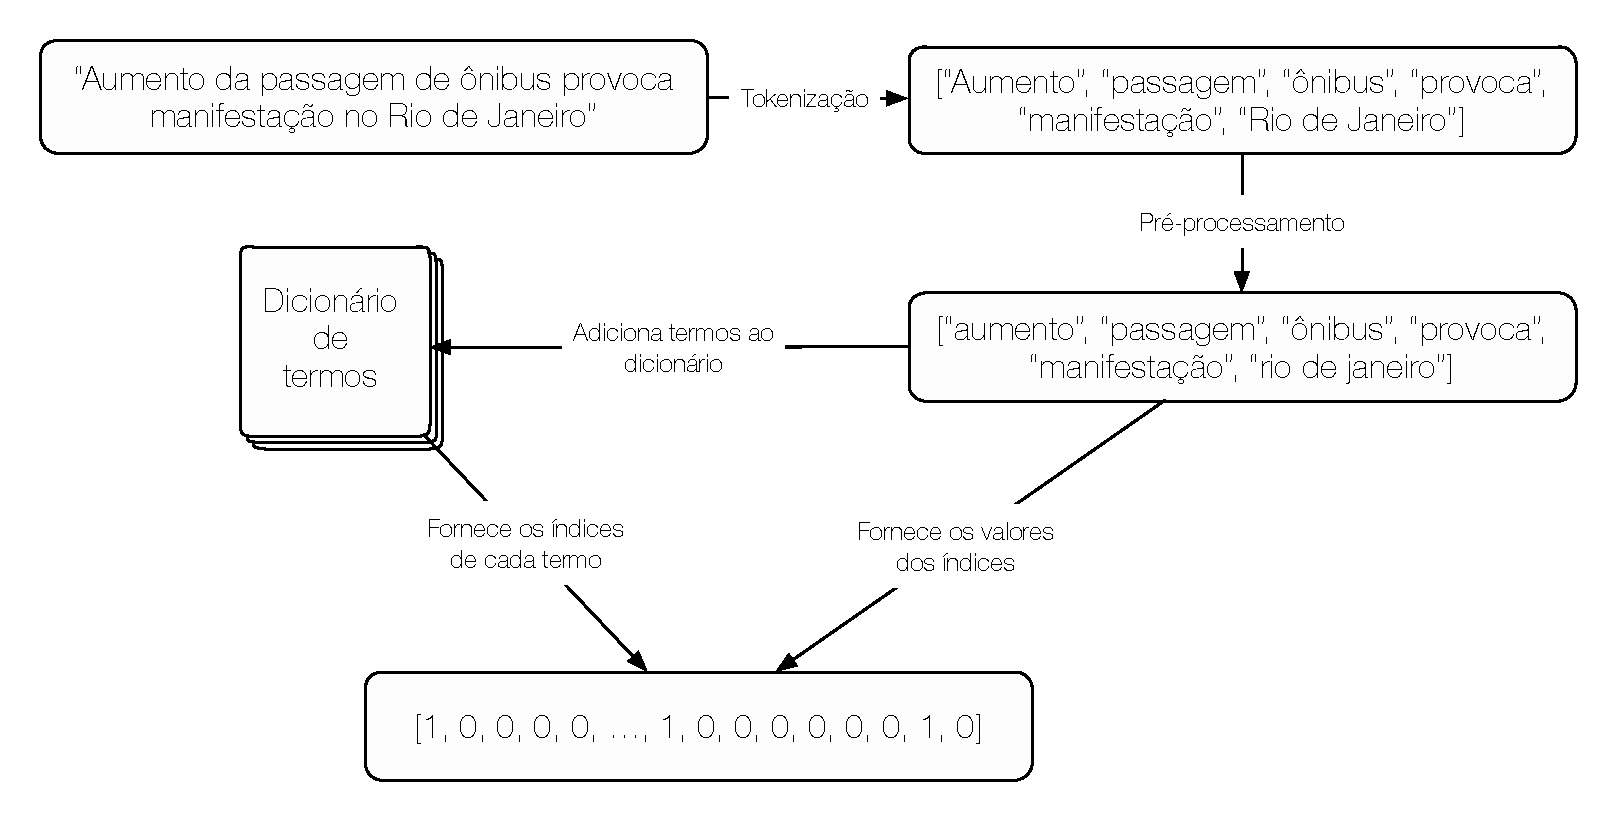
\includegraphics[width=1.0\textwidth]{figuras/conversao-modelo-espaco.eps}
    \caption{Conversão para o modelo de espaço vetorial.}
  \end{center}
\end{figure}

\subsection*{Tokenização e pre-processamento}

Para realizar a \textit{tokenização} dos textos das publicações, é utilizado o método \textit{String\#split}. O método aceita como parâmetro um ou mais caracteres, ou uma expressão regular\footnote{http://turing.com.br/material/regex/introducao.html} para dividir o texto em termos de acordo com esse parâmetro. O texto é quebrado a cada parte que casa com o parâmetro passado. 

O modelo utiliza como parâmetro para o método uma expressão regular separa os termos da publicação, primeiramente, de acordo com a lista de cidades do Brasil, e posteriormente por espaços, como está indicado no código a seguir. Se uma cidade é encontrada na publicação, é gerado apenas um termo, por exemplo, ``Rio de Janeiro'' gera apenas um termo.

\begin{lstlisting}
  /(\bCidade 1\b)|(\bCidade 2\b)|...|(\bCidade N-1\b)|(\bCidade N\b)|\s/
\end{lstlisting}

Na expressão regular, encontram-se os seguintes operadores:

\begin{itemize}
  \item \textbf{``$\mid$''}: captura uma expressão ou outra.
  \item \textbf{``\textbackslash s''}: captura espaços
  \item \textbf{``\textbackslash b''}: captura quebra de expressão como espaço, início ou fim de linha
  \item \textbf{``('' e ``)''}: identificador para retornar a expressão neles contida
\end{itemize}

Ao pedir para o método dividir a expressão a partir dessa expressão regular, está se dizendo para dividir a expressão pela ``Cidade 1'' ou a ``Cidade 2'' ou a ``Cidade 3'', e assim por diante até a ``Cidade N'', ou por espaço, ao final. O resultado da divisão de termos para a publicação ``Manifestação hoje no Rio de Janeiro'' será:

\begin{lstlisting}
  expressao = "Manifestação hoje no Rio de Janeiro"
  expressao.split(/(Rio de Janeiro)|(São Paulo)\s/)
  # => ["Manifestação", "hoje", "no", "Rio de Janeiro"]
\end{lstlisting}

Para criar os termos das cidades do Brasil, é utilizada uma lista de cidades\footnote{http://samus.com.br/web/site/artigo-todas\_as\_cidades\_do\_brasil\_atualizado\_e\_com\_acentos}, que é salva em uma estrutura JSON em que as chaves são as cidades e os valores são os estados, para posteriormente mapear as cidades aos estados. O processo de conversão do JSON para a expressão regular está identificado Figura 5.2.

\begin{figure}[htpb]
  \begin{center}
    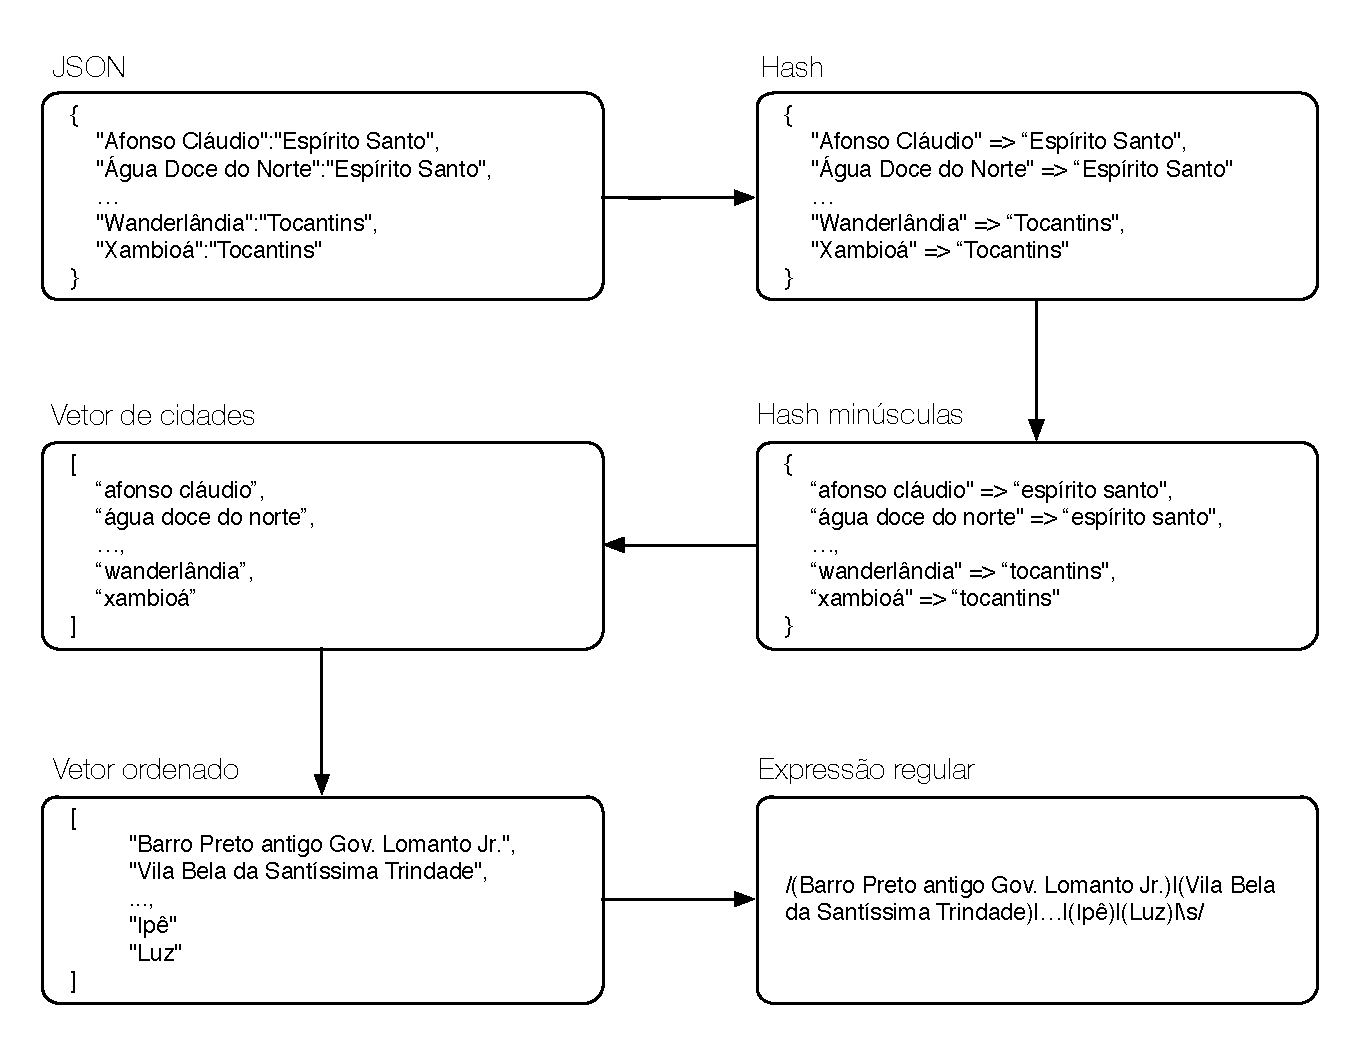
\includegraphics[width=0.9\textwidth]{figuras/criacao-regexp.eps}
    \caption{Criação da expressão regular.}
  \end{center}
\end{figure}

Para converter as cidades da estrutura JSON para \textit{Hash}, são utilizados os métodos \textit{IO.read}, que se encarrega de ler o arquivo, e \textit{JSON.parse}, que trata de convertê-lo, como indicado na linha 2 do código a seguir. A seguir, todas as chaves e valores do \textit{Hash} são iterados pelo método \textit{Hash\#each\_with\_object} para convertê-los para minúsculas, como indicado nas linha 3, 4 e 5. Para retirar as cidades, é utilizado o método \textit{Hash\#keys}, como indicado na linha 6 do código a seguir:

\begin{lstlisting}
  class String
    JSON_CIDADES = JSON.parse(IO.read("support/cidades_do_brasil.json"))
    ESTADOS_E_CIDADES = JSON_CIDADES.each_with_object({}) do |(k,v), h|
      h[k.downcase] = v.downcase
    end
    LISTA_DE_CIDADES = ESTADOS_E_CIDADES.keys.sort_by { |c| c.length }.reverse
    (...)
  end
\end{lstlisting}

A lista de cidades é ordenada da cidade com o maior nome para a menor, pois a ordem das cidades na expressão regular influencia no modo de criação dos termos a partir do texto da publicação. Isso é preciso ser feito, para que cidades como ``Porto Alegre'' sejam identificadas corretamente, sendo que a cidade ``Porto'' também existe. Caso contrário, a expressão iria identificar o termo ``Porto'' da cidade ``Porto Alegre'' como sendo uma cidade separada, ao invés de identificar que o mesmo termo está junto com o termo ``Alegre'', o que o caracteriza como uma outra cidade.

Para ordená-los dessa maneira, é utilizado o método \textit{Array\#sort\_by}, passando o tamanho de cada termo dentro do bloco, e a seguir é aplicado o método \textit{Array\#reverse} para reordená-los do maior para o menor, como indicado na linha 6 do código anterior.

A seguir as cidades são unidas através da iteração do vetor e na substituição de cada termo por seu constituinte dentro da expressão regular: ``Rio de Janeiro'' se torna ``\b(Rio de Janeiro)\b''. Os termos são então unidos em uma única cadeia de caracteres através do método \textit{Array\#join}, passando como parâmetro o operador ``ou'' da expressão regular, como indicado na linha 3 do código a seguir. Por fim, na linha 4, é criada a expressão regular a partir das cidades unidas, com o final da expressão indicando ``ou espaço'':

\begin{lstlisting}
  class String
    # (...)
    CIDADES_UNIDAS = LISTA_DE_CIDADES.map { |city| "(\\b#{city}\\b)" }.join("\|")
    CIDADES_EXPREG = Regexp.new "#{CIDADES_UNIDAS}|\\s"
  end
\end{lstlisting}

Após a conversão dos termos, os mesmos tem todos os caracteres de pontuação retirados utilizando o método \textit{String\#gsub}. O método recebe dois parâmetros: o primeiro é o trecho que se deseja substituir, e o segundo o trecho para qual irá substituí-lo. No primeiro parâmetro é passada uma expressão regular que representa todos os caracteres de pontuação. No segundo, não é passado caractere nenhum, o que indica que se deseja remover os trechos passados no primeiro parâmetro, como indicado na linha 3 do código a seguir.

Alguns termos também são ignorados, como preposições e pronomes. Os termos que são ignorados são identificados a partir de um vetor de exceções. Para deletar os respectivos termos do vetor de termos, é utilizado o método \textit{Array\#delete\_if}, que recebe um bloco e deleta o elemento do vetor caso o resultado operação lógica dentro do bloco retorne verdadeiro, como indicado na linha 4 do código a seguir.

A expressão lógica utilizada para determinar se o termo é deletado ou não, inclui a verificação se o termo se encontra no vetor de exceções, através do método \textit{Array\#include?}, e também da verificação se o termo possui sequências de caracteres como ``http://'' ou ``kk'' ou ``haha'', através do método \textit{String\#include?}, como indicado nas linhas 5 e 6 do código a seguir:

\begin{lstlisting}
  class String
    def tokenizar
      termos = self.downcase.split(CIDADES_EXPREG).map! { |termo| termo.gsub(/\p{^Alnum}\s/, '') }
      termos.delete_if do |termo| 
        termo == "" || EXCECOES.include?(termo) || termo.include?("http") || 
        termo.include?("@") || termo.include?("kk") || termo.include?("haha")
      end
    end
  end
\end{lstlisting}

\subsection*{Dicionário de termos e vetor de características}

O dicionário de termos é criado à partir do conjunto de termos de todas as publicações. Os termos de todas as publicações são recolhidos, como indica as linhas 4 e 5 do código, e são utilizados os métodos \textit{Array\#flatten}, \textit{Array\#uniq} e \textit{Array\#sort} para criar o dicionário, como indica a linha 6 do código:

\begin{lstlisting}
  class Treinador
    #(...)
    def criar_dicionario_de_termos
      @dicionario_de_termos = @publicacoes_de_treino.map do |publicacao| 
        publicacao.termos
      end.flatten.uniq.sort
    end
    #(...)
  end
\end{lstlisting}

O método \textit{Array\#flatten} é utilizado para reduzir vetores à apenas uma dimensão. Ele é necessário pois as publicações encontram-se cada uma em um vetor de termos, sendo a lista de todas uma matriz de termos. \textit{Array\#uniq} é utilizado para reduzir os termos à apenas uma ocorrência de cada um, e \textit{Array\#sort} para ordenar os termos por ordem alfabética.

Com o dicionário construído, o vetor de características de cada publicação é obtido através da iteração entre os termos do dicionário e a atribuição do valor ``1'' caso os termos da publicação incluam o respectivo termo do dicionário, e ``0'' caso não incluam, como indica a linha 5 do código a seguir. Posteriormente, é preciso converter o vetor para a estrutura interna do LIBSVM, como está na linha 7 do código:

\begin{lstlisting}
  class Publicacao
    # (...)
    def vetor
      vetor = @treinador.dicionario_de_termos.map do |termo| 
        @termos.include?(termo) ? 1 : 0
      end
      Libsvm::Node.features(vetor)
    end
    # (...)
  end
\end{lstlisting}

\subsection*{Extração}

Para obter a cidade e o estado da publicação é identificado, primeiramente, se os termos da informação da localização do usuário incluem alguma cidade da lista de cidades previamente criadas. Para isso, é aplicada a tokenização na informação da localização e utizado o método \textit{Array\#include?} para verificar se a lista de cidades inclui o termo da localização. Caso localização definida pelo usuário não inclua cidade alguma, é verificado através do mesmo método se a publicação inclui alguma cidade, como indicado no código a seguir:

\begin{lstlisting}
  class Publicacao
    def initialize
      # (...)
      @cidade = extrair_cidade
    end

    def extrair_cidade
      cidade = ""
      if @localizacao_no_perfil
        @localizacao_no_perfil.tokenizar.each do |termo|
          if String::LISTA_DE_CIDADES.include?(termo)
            cidade = termo
          end
        end
      end
      if cidade == ""
        @termos.each do |termo|
          if String::LISTA_DE_CIDADES.include?(termo)
            cidade = termo
          end
        end
      end
      cidade
    end
    # (...)
  end
\end{lstlisting}

\section{Classificação com SVM}

A classificação das publicações é feita uiltizando a interface Ruby da biblioteca LIBSVM ``rb-libsvm''\footnote{https://github.com/febeling/rb-libsvm}, na versão 1.1.5. A interface permite manipular a biblioteca a partir de classes e métodos Ruby. A LIBSVM implementa uma variedade SVMs, regressão de vetores de suporte (SVR) e classificação de vetores de suporte (SVC), é compatível com SVMs de duas ou mais classes e disponibiliza diversas funções de kernel para a sua utilização, possuindo implementações nas linguagens C++ e Java e interfaces para Ruby, Python, PHP, MATLAB, etc.

A interface ``rb-libsvm'' já inclui a biblioteca LIBSVM, eliminando a necessidade da instalação de qualquer outro programa. Para configurar o ambiente para a classificação com o uso de SVM em Ruby, roda-se o seguinte código a partir do terminal:

\begin{lstlisting}
  gem install rb-libsvm --version 1.1.5
\end{lstlisting}

\subsection*{Treinamento}

Para o treinamento do SVM, são utilizadas as classes criadas pela interface com o LIBSVM, são elas: \textit{Libsvm::Problem} e \textit{Libsvm::Parameter}.

A classe \textit{Libsvm::Problem} é encarregada de receber o conjunto de $n$ descritores $({x}_{i}, {y}_{i})$, compostos pelos vetores de características ${x}_{i}$ e a suas respectivas classes ${y}_{i}$, como por exemplo da forma da Tabela 5.2:

\begin{table}[ht]
  \caption{Conjunto de descritores}
  \centering
  \begin{tabular}{| c | c | c |}
    \hline
    \textbf{Sejam} & \textbf{${x}_{i}$} & \textbf{${y}_{i}$} \\ [0.5ex] \hline \hline
    1 & [1, 0, 0, 1, 0, 0, ..., 0, 0, 1] & 1.0 \\ \hline
    2 & [0, 0, 0, 1, 1, 0, ..., 0, 1, 0] & 1.0 \\ \hline
    3 & [0, 1, 0, 1, 0, 0, ..., 0, 0, 0] & -1.0 \\ \hline
    ... & ... & ... \\ \hline
    n-1 & [0, 0, 1, 0, 0, 0, ..., 1, 0, 1] & -1.0 \\ \hline
    n & [1, 0, 0, 0, 0, 0, ..., 1, 1, 1] & 1.0 \\ \hline
    \hline
  \end{tabular}
  \label{table:nonlin}
\end{table}

\begin{table}[ht]
  \caption{Conjunto de descritores}
  \centering
  \begin{tabular}{| c |}
    \hline
    \textbf{${x}_{i}$} \\ [0.5ex] \hline \hline
    [1, 0, 0, 1, 0, 0, ..., 0, 0, 1] \\ \hline
    [0, 0, 0, 1, 1, 0, ..., 0, 1, 0] \\ \hline
    [0, 1, 0, 1, 0, 0, ..., 0, 0, 0] \\ \hline
    ... \\ \hline
    [0, 0, 1, 0, 0, 0, ..., 1, 0, 1] \\ \hline
    [1, 0, 0, 0, 0, 0, ..., 1, 1, 1] \\ \hline
    \hline
  \end{tabular}
  \label{table:nonlin}
\end{table}

A classe \textit{Libsvm::Parameter} encapsula os ajustes dos parâmetros do SVM. Para o modelo implementado, apenas o parâmetro de custo ($C$) (indicado na Equação 4.1) é ajustado, porém também é necessário inicializar os valores dos parâmetros \textit{epsilon} e \textit{cache size}, porém seus valores não são alterados da sua configuração inicial. O código a seguir apresenta a inicialização das classes do LIBSVM e dos parâmetros:

\begin{lstlisting}
  class Classificador
    # (...)
    def initialize
      # (...)
      @problema = Libsvm::Problem.new
      @parametro = Libsvm::SvmParameter.new
      inicializa_parametros
    end

    def inicializa_parametros
      @parametro.cache_size = 1
      @parametro.eps = 0.001
      @parametro.c = 0.1 # cost
    end
    # (...)
  end
\end{lstlisting}

Para carregar as publicações de treino, as publicação são lidas a partir do arquivo CSV e é instanciada uma classe \textit{Publicação} para cada linha do arquivo:

\begin{lstlisting}[caption=Carregamento de publicações]
  class Treinador
    # (...)
    def carregar_publicacoes_de_treino caminho
      CSV.open(caminho) do |csv|
        csv.each do |linha|
          @publicacoes_de_treino << Publicacao.new(linha, self)
        end
      end
    end
    # (...)
  end
\end{lstlisting}

Como o processo de extração do vetor de características de cada publicação já está definido, basta obter agora as suas classes, que estão contidas na posição 6 de cada linha do arquivo CSV. Para obtê-las, então, basta iterar entre as publicações e guardar a posição 6 de cada uma, como indicado na linha 4 do código a seguir:

\begin{lstlisting}
  class Treinador
    # (...)
    def classes
      @publicacoes_de_treino.map { |publicacao| publicacao.linha_csv[6].to_i }
    end
    # (...)
  end
end
\end{lstlisting}

Com as publicações carregadas e com seus respectivos descritores ${x}_{i}$ e ${y}_{i}$ definidos, o SVM é treinado a partir da inserção dessas informações. O classificador irá, de acordo com os descritores, e do parâmetro $C$ definido anteriormente, encontrar a resolução para a equação 4.1, calculando os valores de $w$ e $b$. Como está representado na Figura 5.3:

\begin{figure}[htpb]
  \begin{center}
    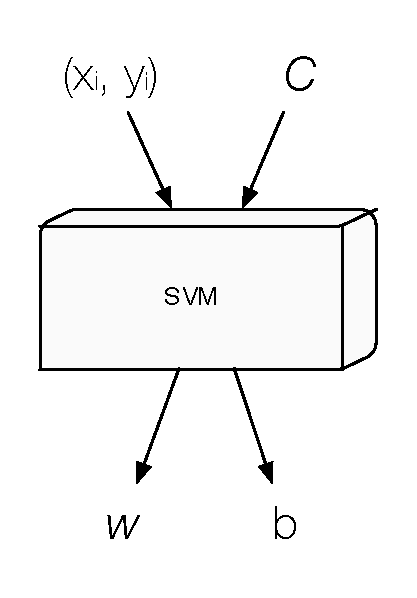
\includegraphics[width=0.25\textwidth]{figuras/svm-extracaowb.eps}
    \caption{Cálculo de $w$ e $b$ a partir dos descritores e $C$}
  \end{center}
\end{figure}

Para inserir os descritores no LIBSVM, junto com os parâmetros, e treinar o classificador são utilizados os métodos \textit{Libsvm::Problem\#set\_examples} e \textit{Libsvm::Model.train}. O primeiro recebe apenas os descritores e os une na estrutura interna da biblioteca, mostrado na linha 4 do código a seguir, e o segundo recebe esses dados em conjunto com os parâmetros, mostrado na linha 5 do código:

\begin{lstlisting}
  class Classificador
    # (...)
    def definir_modelo
      @problema.set_examples(@treinador.classes, @treinador.vetores_de_treino)
      @modelo = Libsvm::Model.train(@problema, @parametro)
    end
    # (...)
  end
\end{lstlisting}

Nesse momento, através do método \textit{Libsvm::Model.train}, $w$ e $b$ já estão definidos e armazenados na instância do modelo. O SVM já está com as informações disponíveis para classificar futuras ocorrências, porém resta apenas saber se o mesmo possui uma boa taxa de acerto ou não. 

Para elevar a taxa de acerto do classificador, o mesmo é treinado e testado com diversos valores para o parâmetro $C$, utilizando o mesmo conjunto de descritores. A finalidade é encontrar valores de $w$ e $b$ que retornem as classes ${y}_{i}$ dos vetores de características ${x}_{i}$ mais próximas da realidade. Os resultados da fase de teste para os valores do parâmetro $C$ escolhidos são exibidos na Tabela 5.3.

Para propriamente implementação da fase teste do classificador é a mesma que propriamente o processo de classificação, por isso os dois processos são explicados de forma única na seção seguinte.

\subsection*{Classificação e teste}

Ambas fases de teste e classificação utilizam o mesmo código, se diferenciando apenas pelo conjunto de publicações que carregados. Para carregar as publicações é utilizado o mesmo processo feito entre as linhas 4 e 8 do Código 5.1.

Para propriamente classificar as publicações, ou seja, obter suas classes, é utilizado o método \textit{Libsvm::Problem\#predict}. Como o modelo instanciado já resolveu a Equação 4.1 de acordo com os dados informados, é possível fazer uma chamada ao método passando uma publicação específica e receber o valor de sua classe.

No processo anterior, o modelo foi alimentado com diversas informações de ${x}_{i}$ e ${y}_{i}$, possibilitando que ele gerasse os valores de $w$ e $b$. Como ambos já estão definidos, agora, é possível introduzir um dado de ${x}_{i}$ (uma publicação) e receber de volta o seu ${y}_{i}$, a sua classe, como definido na Equação 4.2 e na Figura 5.4.

\begin{figure}[htpb]
  \begin{center}
    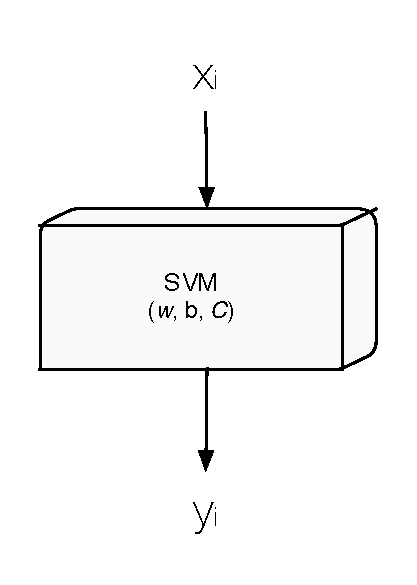
\includegraphics[width=0.25\textwidth]{figuras/svm-testexiyi.eps}
    \caption{Obtenção da classe ${y}_{i}$ através do fornecimento do vetor ${x}_{i}$}
  \end{center}
\end{figure}

Então, ao realizar a chamada para o método \textit{Libsvm::Problem\#predict}, na linha 7 do código a seguir, passando o vetor de uma publicação ${x}_{i}$, é recebida a sua classe ${y}_{i}$ como retorno, com os valores ``1.0'' ou ``-1.0''.

Para registrar a saída das classes, elas são gravadas em um novo arquivo CSV, que contém as informação das publicações e as classes (como é feito manualmente na fase de treino). O código, juntamente ao salvar a classe, também salva a cidade da publicação. No código a seguir, \textit{linha\_csv} representa cada linha do arquivo CSV (uma publicação) no formato de um vetor, até o momento da classificação, cada linha possui 6 posições (da 0 a 5), então as novas informações são adicionadas da sétima posição em diante, como indicado nas linhas 8 e 9 do código a seguir:

\begin{lstlisting}
  class Classificador
    # (...)
    def testar_modelo caminho_saida
      CSV.open(caminho_saida, "w") do |csv|
        @publicacoes.each do |publicacao|
          linha_csv = publicacao.linha_csv
          classe = @modelo.predict(publicacao.vetor)
          linha_csv[6] = classe
          linha_csv[7] = publicacao.cidade
          csv << linha_csv
        end
      end
    end
    # (...)
  end
\end{lstlisting}

Finalmente, para gerar o arquivo CSV final com apenas as publicações positivas - que serão apresentadas no ambiente interativo - são percorridas as publicações e gravados em outro arquivo apenas as que possuem o valor ``1.0'' no campo da sua classificação:

\begin{lstlisting}
  class Classificador
    def filtrar_arquivo_de_classificacoes_positivas caminho_entrada, caminho_saida
      CSV.open(caminho_entrada) do |csv_entrada|
        CSV.open(caminho_saida, 'w') do |csv_saida|
          csv_entrada.each do |linha_entrada|
            csv_saida << linha_entrada if linha_entrada[6] == "1.0"
          end
        end
      end
    end
  end
\end{lstlisting}

\section{Resultados}

Foram obtidas 30.198 publicações do Twitter que contém a palavra-chave ``manifestação'', referentes ao mês de agosto de 2014. Desse conjunto, foram selecionadas 243 publicações de treino positivas e 233 negativas, totalizando 476 publicações de treino. Para a fase de testes, foram selecionadas 70 positivas e 70 negativas, totalizando 140 publicacões de teste.

\subsection*{Testes}

Para a fase de testes, o SVM foi executado diversas vezes, uma para cada valor para o parâmetro $C$. A Tabela 5.1 indica a taxa de acerto obtida para cada valor de $C$, junto com o tempo que necessário para a classificação.

\begin{table}[ht]
  \caption{Taxa de acerto SVM.}
  \centering
  \begin{tabular}{| c | c | c |}
    \hline
    \textbf{$C$} & \textbf{Taxa de acerto} & \textbf{Performance} \\ [0.5ex] \hline \hline
    ... & 50\% & ... \\ \hline
    0.001 & 50\% & 9,4s \\ \hline
    0.01 & 78,5\% & 9,3s \\ \hline
    0.1 & 90,5\% & 8,0s \\ \hline
    1 & 89.5\% & 7,9s \\ \hline
    10 & 86.5\% & 7,6s \\ \hline
    100 & 86.5\% & 7,8s \\ \hline
    1000 & 86.5\% & 7,5s \\ \hline
    ... & 86.5\% & ... \\ [1ex]
    \hline
  \end{tabular}
  \label{table:nonlin}
\end{table}

Foi percebido, que para um valor muito baixo de $C$, o classificador adquire o comportamento de classificar todas as publicações como positivas. Já para um valor muito alto de $C$, a taxa de acerto se manteve em 86,5\%. O valor otimizado para $C$ foi encontrado para o valor ``0.1'', no qual o classificador exibiu a maior taxa de acerto, de 90,5\%. A performance, apesar de variar, não se mostrou muito relevante para o modelo.

\subsection*{Total de publicações e localização}

Após a classificação, as publicações positivas somaram 13.611 e as negativas 16.587. 

As publicações positivas e negativas exibem divergência no que diz respeito a extração da cidade e geolocalização. As positivas exibiram maior possibilidade de extração da sua cidade, através do texto da publicação ou do perfil do usuário. Já as negativas, exibiram quase 3 vezes mais o dado de geolocalização, apesar de ainda ser em baixa quantidade (3.6\%).

Ainda nas publicações positivas, para os dados de localização contidos na publicação ou no perfil do usuário, foi possível a extração da informação em 8.148 publicacões (60\% delas). A Tabela 5.3 indica os resultados para os dados extraídos:

\begin{table}[ht]
  \caption{Resultados da classificação e dos dados extraídos.}
  \centering
  \begin{tabular}{| c || c | c | c |}
    \hline
    \textbf{Publicações} & \textbf{Quantidade} &  \textbf{Com cidade} & \textbf{Com geolocalização} \\ [0.5ex] \hline \hline
    \textbf{Positivas} & 13.611 & 8148 (60\%) & 177 (1.3\%) \\ \hline
    \textbf{Negativas} & 16.587 & 8700 (52.4\%) & 610 (3.6\%) \\ \hline
    \textbf{Total} & 30.198 & 16.848 (56\%) & 787 (1.9\%) \\ [1ex]
    \hline
  \end{tabular}
  \label{table:nonlin}
\end{table}

Das publicações positivas, apenas 177 delas (cerca de 1\%) contem a geolocalização. Isso demonstra que a grande maioria das publicações ainda está sendo enviada pelo computador ou por dispositivos sem o GPS ativado.

\subsection{Análise visual e ambiente}

Segundo \citeonline{Thomas2005}, \textit{Análise Visual} é ``a ciência do raciocínio analítico facilitada por interfaces visuais interativas''. A área tem recebido crescente atenção por conta do processo de \textit{Big Data}, aonde é estudado como processar grandes volumes de informações, de modo que possam ser geradas análises em cima das mesmas. Como apontam \citeonline{Zhicheng2013} e \citeonline{Begoli2012}, uma das formas de análise é a visual, aonde, torna-se possível tirar conclusões através do raciocínio permitido por meio da visão e da organização de informações favoráveis a isso. 

No ambiente interativo, criado a partir do modelo implementado, é possível analisar visualmente o comportamento das publicações segundo o seu horário e localização. É possível enxergar a existência de picos de publicações em determinados horários, o que podem indicar eventos, e de onde estão surgindo essas publicações, para examinar a localização de cada evento.

Para analisar os eventos, no ambiente interativo (disponível em: \url{http://deteccao.zangrandi.me/}) são exibidos gráficos de séries-temporais das publicações, criados a partir da ferramenta \textit{Highcharts}\footnote{http://www.highcharts.com}, e mapas de marcadores, criados a partir do \textit{TileMill}\footnote{https://www.mapbox.com/tilemill/}.

\subsubsection*{Análise do horário}

Se houve um grande pico de publicações em uma determinada faixa de horário, a possibilidade é que naquela faixa haja a ococrrência de um ou mais eventos. E quanto maior o pico de publicações, maior a magnitude do evento. Através da taxa de acerto obtida na fase de teste da classificação, é possível dizer que 90\% das publicações dizem respeito ao evento de manifestação que o modelo se propõe a detectar.

O gráfico da Figura 5.5 mostra a frequência de publicações relacionadas à manifestações durante cada dia do mês de agosto:

\begin{figure}[htpb]
  \begin{center}
    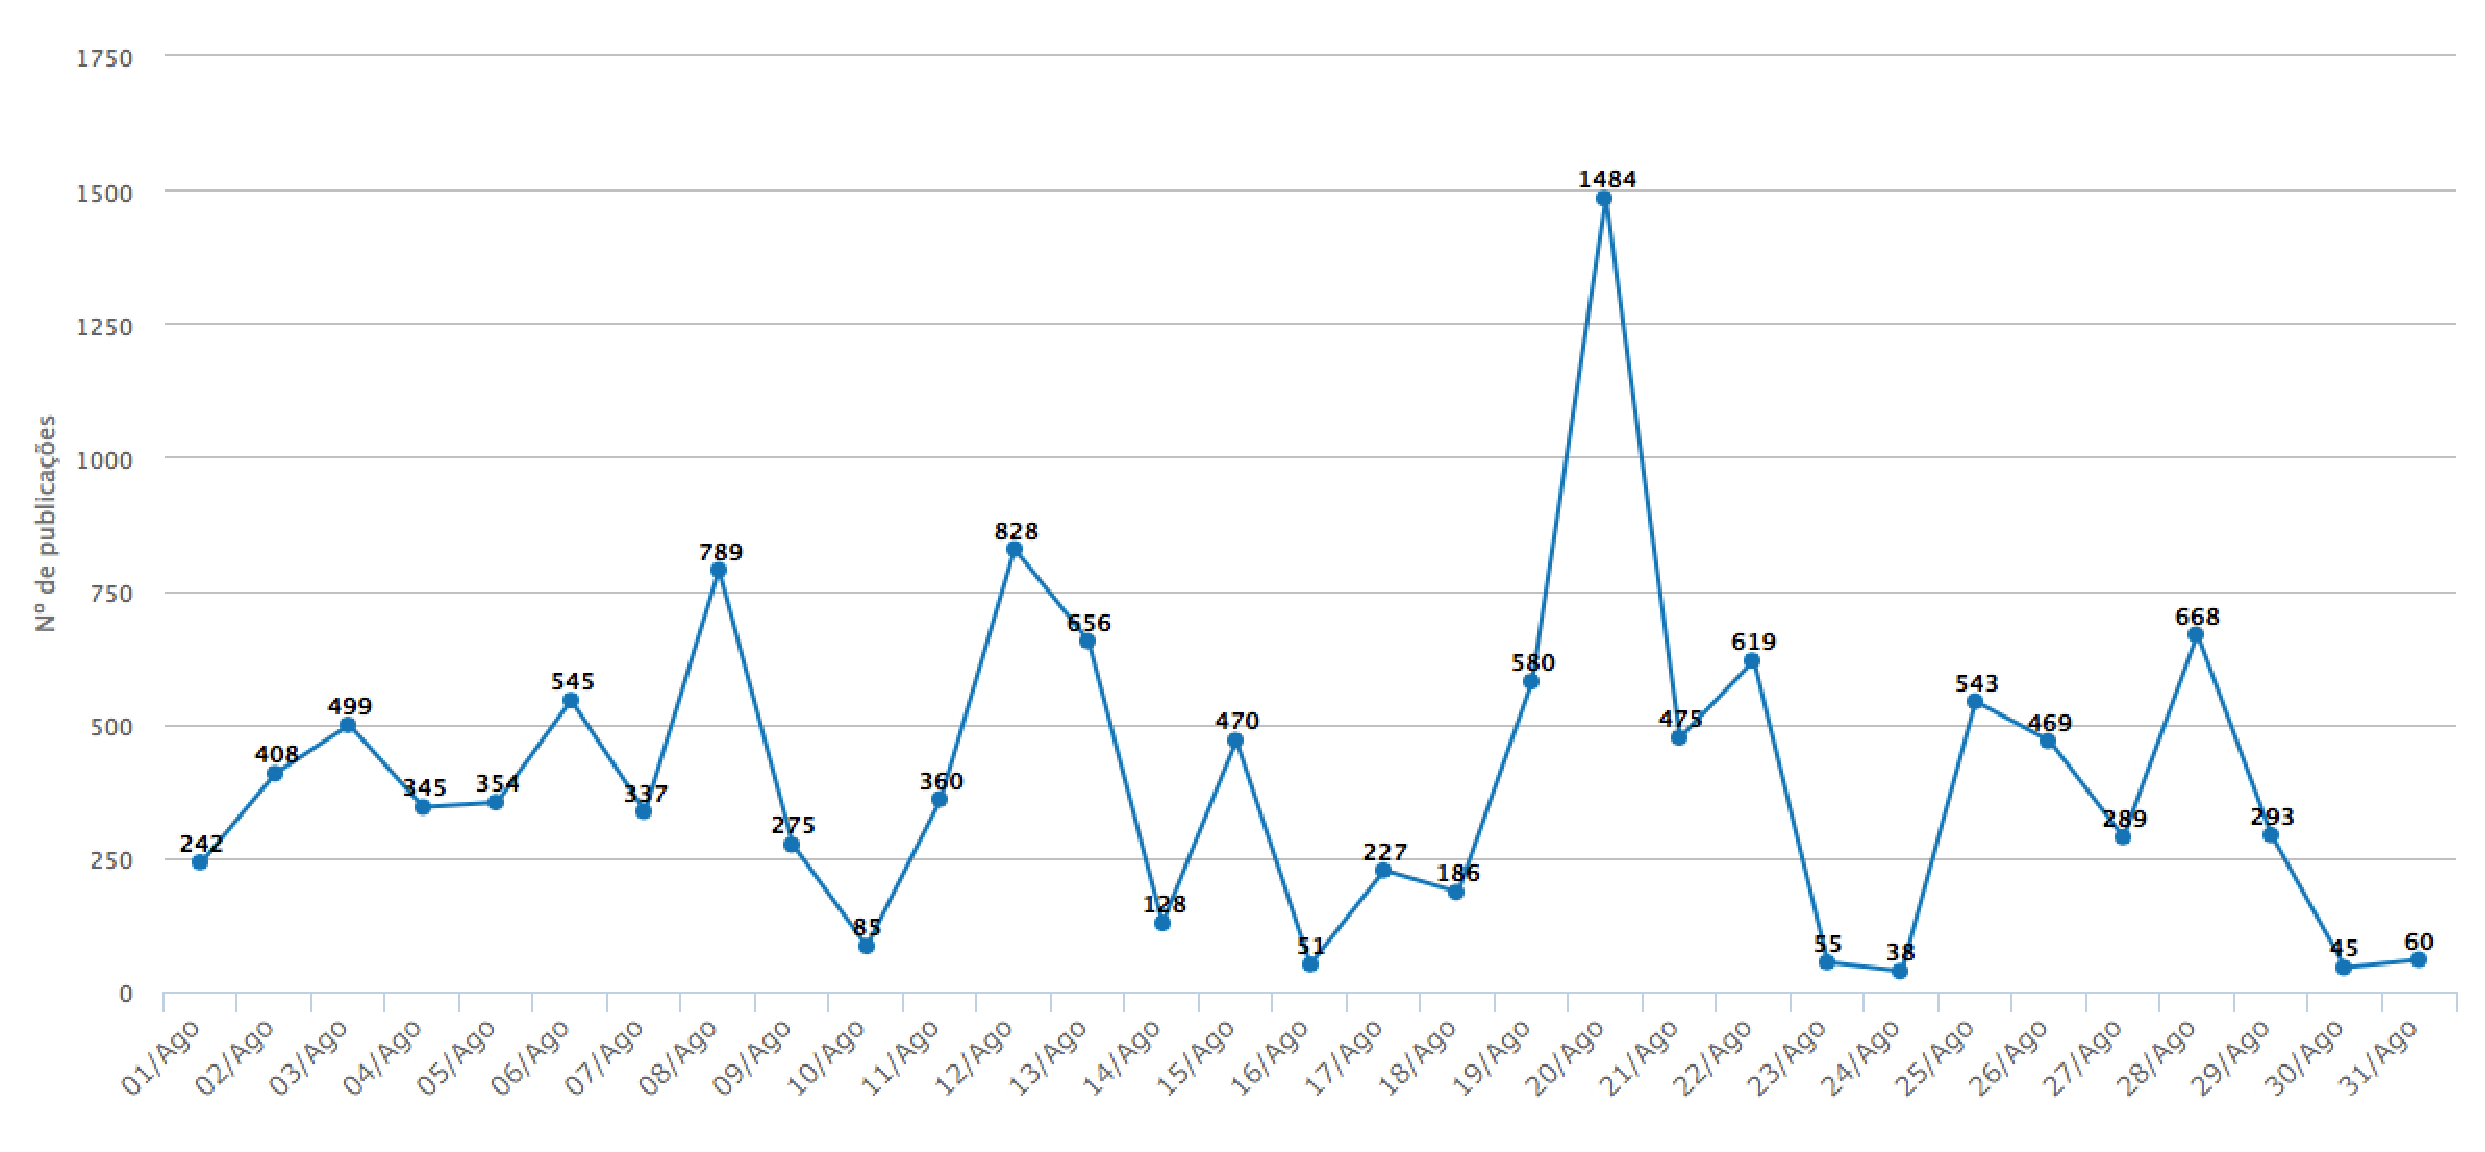
\includegraphics[width=1.0\textwidth]{figuras/grafico-mes.pdf}
    \caption{Publicações do mês de agosto.}
  \end{center}
\end{figure}

É possível observar variações na quantidade de publicações enviadas em cada dia. Particularmente, no dia 20 de agosto, há um grande pico de publicações, podendo indicar algum evento relevante naquele dia. Os dias 08 e 12 também apresentam um número de publicações acima da média. Porém, como o Twitter possui comportamento dinâmico, para chegar à análise dos eventos propostos pelo modelo - manifestações com local e horário - a frequência das publicações devem ser analisadas por dentro de cada dia, por faixa de horário. 

No ambiente interativo, ao clicar em qualquer ponto no gráfico mensal, é exibido o \textit{gráfico diário} daquele dia. Nesse gráfico, também no formato de série-temporal, são apresentadas as publicações por faixa de horário de 1h. Ao analisar as publicações do dia 20 de agosto, por exemplo o seguinte gráfico da Figura 5.6 é apresentado.

\begin{figure}[htpb]
  \begin{center}
    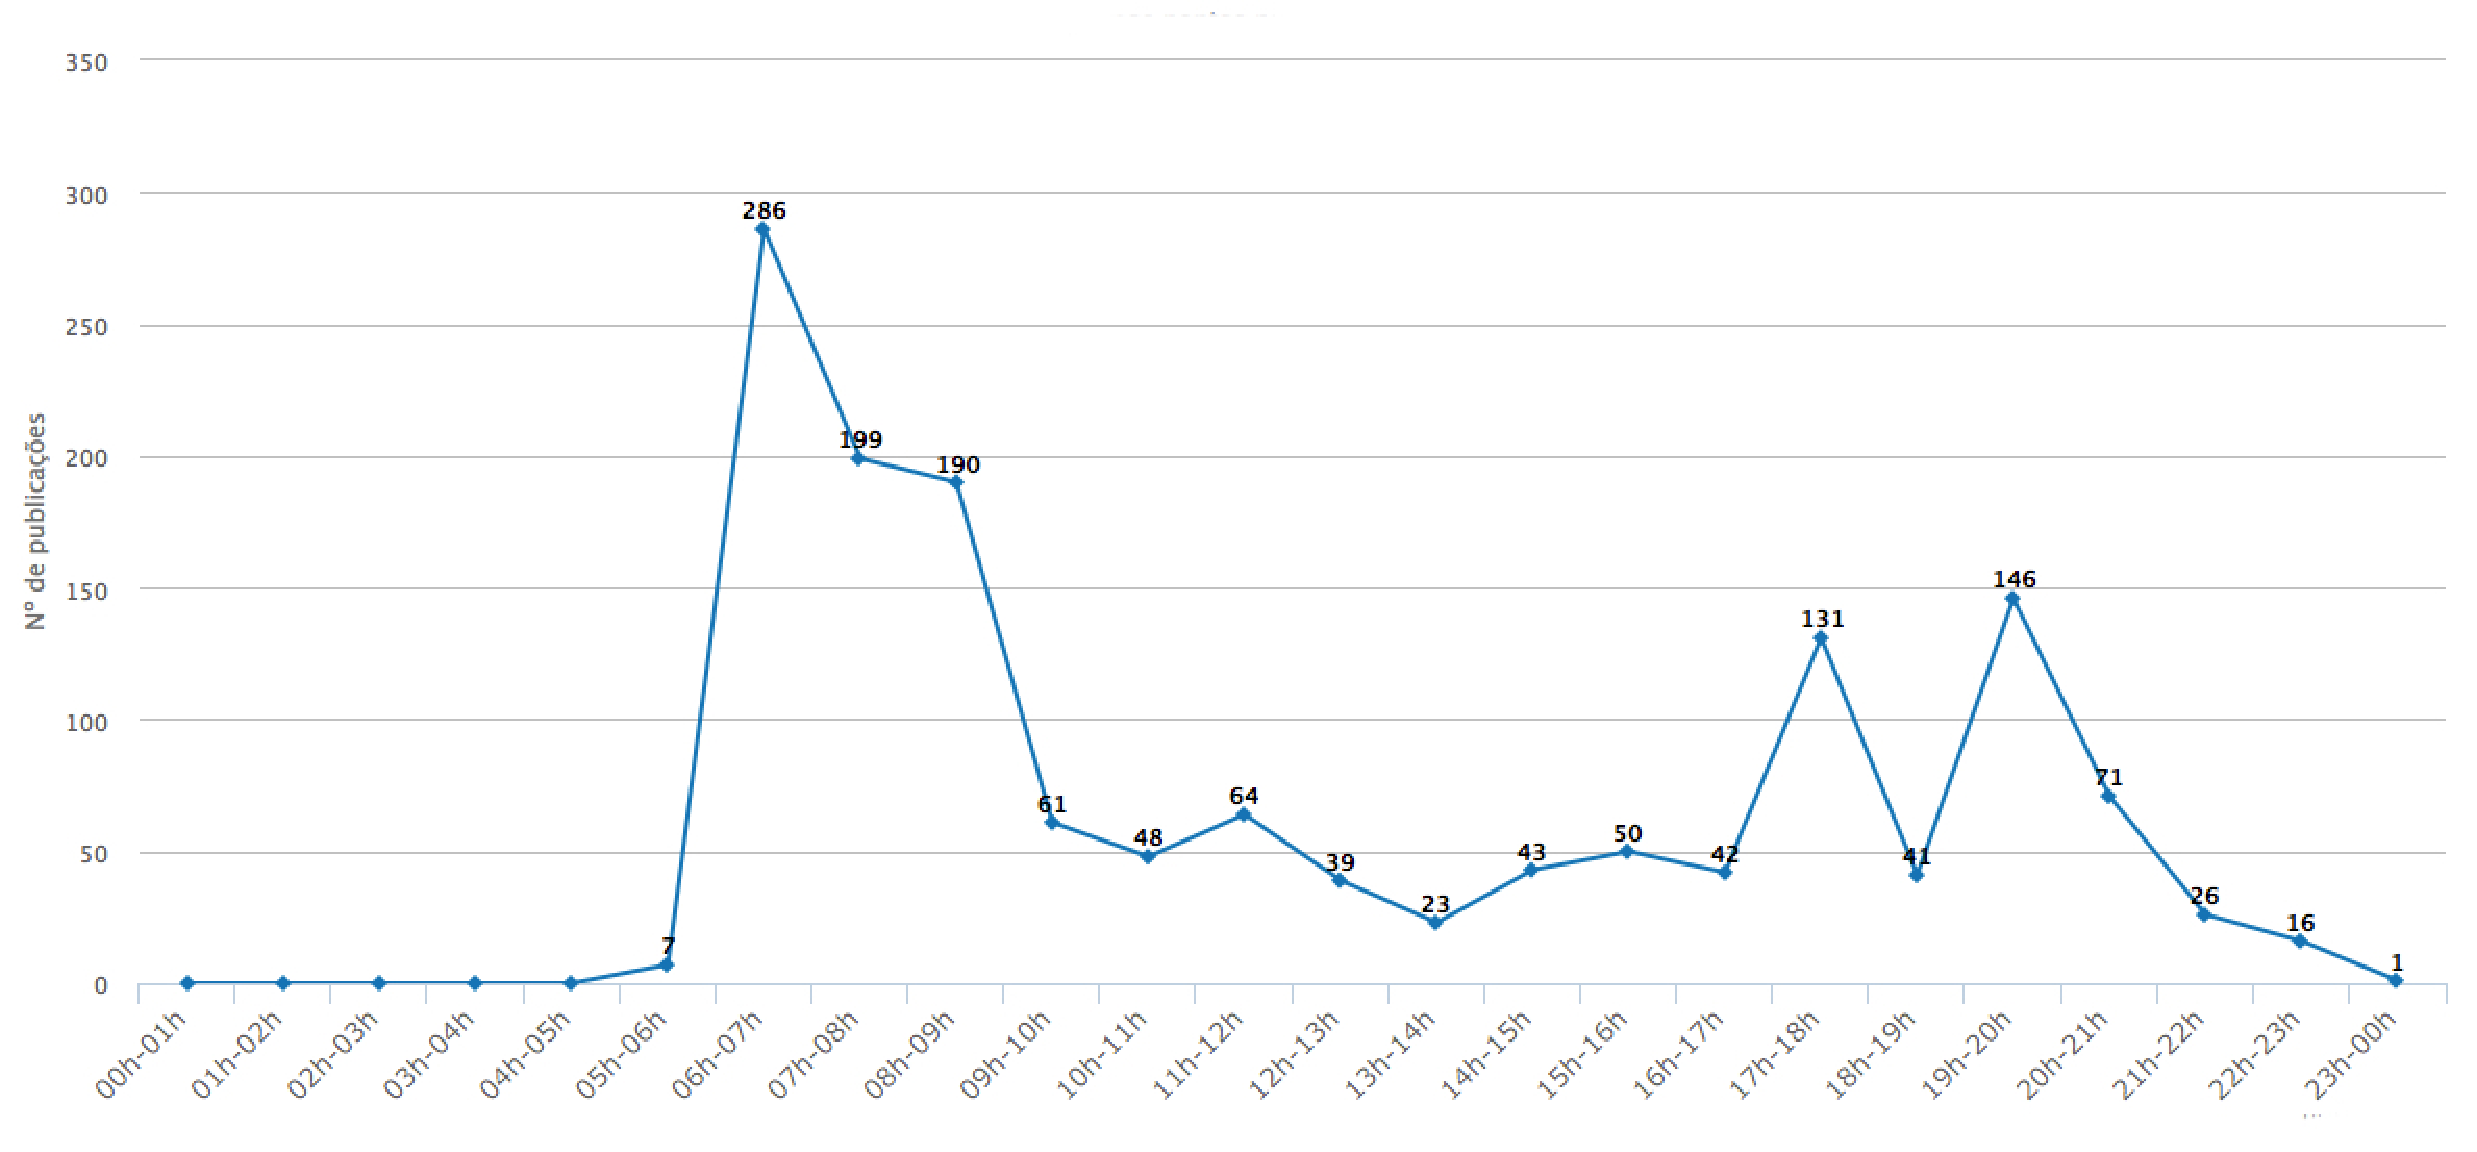
\includegraphics[width=1.0\textwidth]{figuras/grafico-dia.pdf}
    \caption{Publicações do dia 20 de agosto.}
  \end{center}
\end{figure}

No gráfico, é possível visualizar o aparecimento de um grande pico de publicações na faixa de 06h às 07h do dia 20 de agosto. O pico de publicacões reverbera até a faixa de 08h-09h, e novamente ocorrem dois picos nas faixas 17h-18h e 19h-20h.

Com os picos de publicações visíveis e o horário dos eventos aparente, para analisar de onde estão surgindo as publicações e sobre qual evento específico elas estão se referindo, as publicações são exibidas distribuídas no \textit{mapa de marcadores}.

Para o modelo implementado, os vales, ou seja, os pontos de baixa no número de publicações não são relevantes. Em relação ao evento de manifestação, quando não há a sua menção, simplesmente a sua ocorrência não necessita ser detectada. Porém, em aplicações em outros âmbitos como políticos ou comerciais, os vales podem ser interessantes na medida em que determinam uma baixa de popularidade, e talvez seja possível uma ação específica para esse caso.

\subsubsection*{Análise do evento e da localização}

Ao clicar em qualquer ponto do gráfico por faixa de horário, é exibido um mapa de marcadores, no qual é possível visualizar o conteúdo de cada publicação disponível, bem como sua localização exata, para publicações com geolocalização, ou aproximada, para publicações com o registro da cidade. 

As publicações que não contém a geolocalização são aproximadas através do mapeamento das cidades para a sua geolocalização, de acordo com a informação do IBGE\footnote{http://ibge.gov.br/}. O órgão fornece a informação de geolocalização de cada cidade brasileira. A informação serve para marcar corretamente a cidade no mapa apresentado.

Cada mapa de marcador pode exibir os seguintes objetos:

\begin{itemize}
  \item \textbf{Marcador azul escuro:} Publicação única com localização exata.
  \item \textbf{Marcador azul claro:} Publicação única com localização aproximada.
  \item \textbf{Círculo verde:} Pequeno agrupamento de publicações (entre 2 e 10).
  \item \textbf{Círculo amarelo:} Médio agrupamento de publicações (entre 10 e 100).
  \item \textbf{Círculo vermelho:} Grande agrupamento de publicações (maior do que 100).
\end{itemize}

Ao clicar no ponto das publicações entre as 06h e 07h do dia 20 de agosto o mapa da Figura 5.7 é exibido:

\begin{figure}[h!]
  \begin{center}
  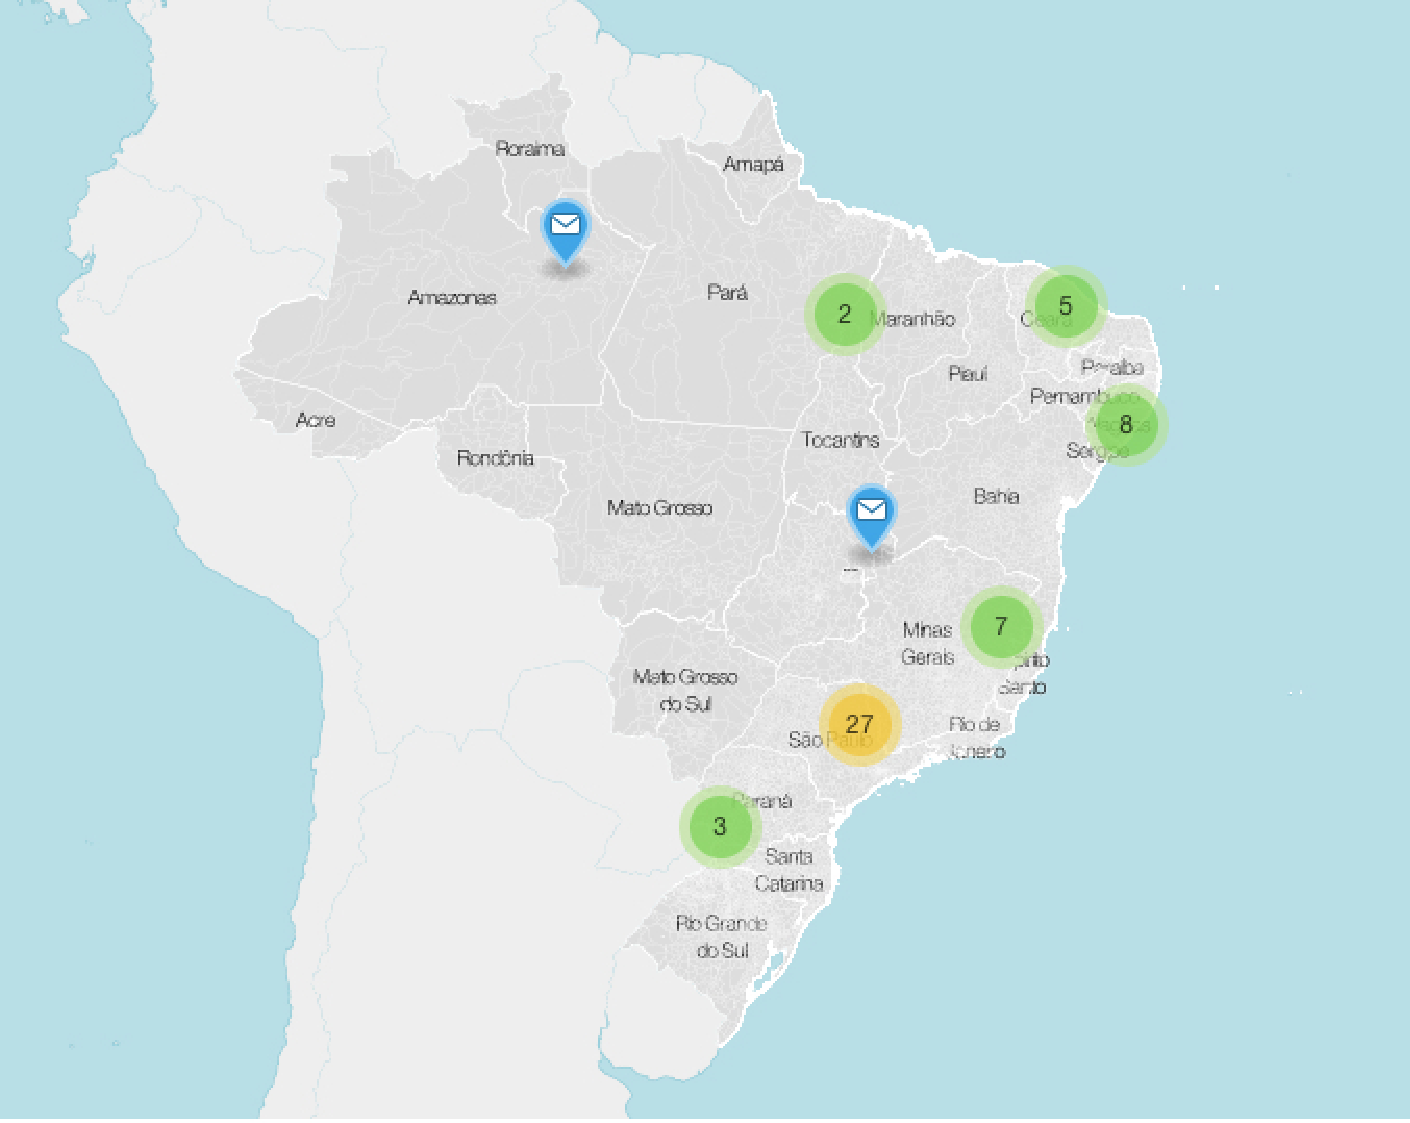
\includegraphics[width=0.8\textwidth]{figuras/mapa-marcador.pdf}
  \caption{Mapa de marcadores para o horário entre 06h e 07h do dia 20/08.}
  \end{center}
\end{figure}

É possível visualizar uma maior concentração de publicações vindas de determinada área do estado São Paulo. Ao aplicar zoom no mapa, o agrupamento de publicações se desfaz, permitindo que as publicacões sejam visualizadas de modo agrupado com mais exatidão, ou também de modo único. 

Ao ampliar o mapa no sentido dessa concentração, o mapa da Figura 5.8 é exibido.

\begin{figure}[h!]
  \begin{center}
  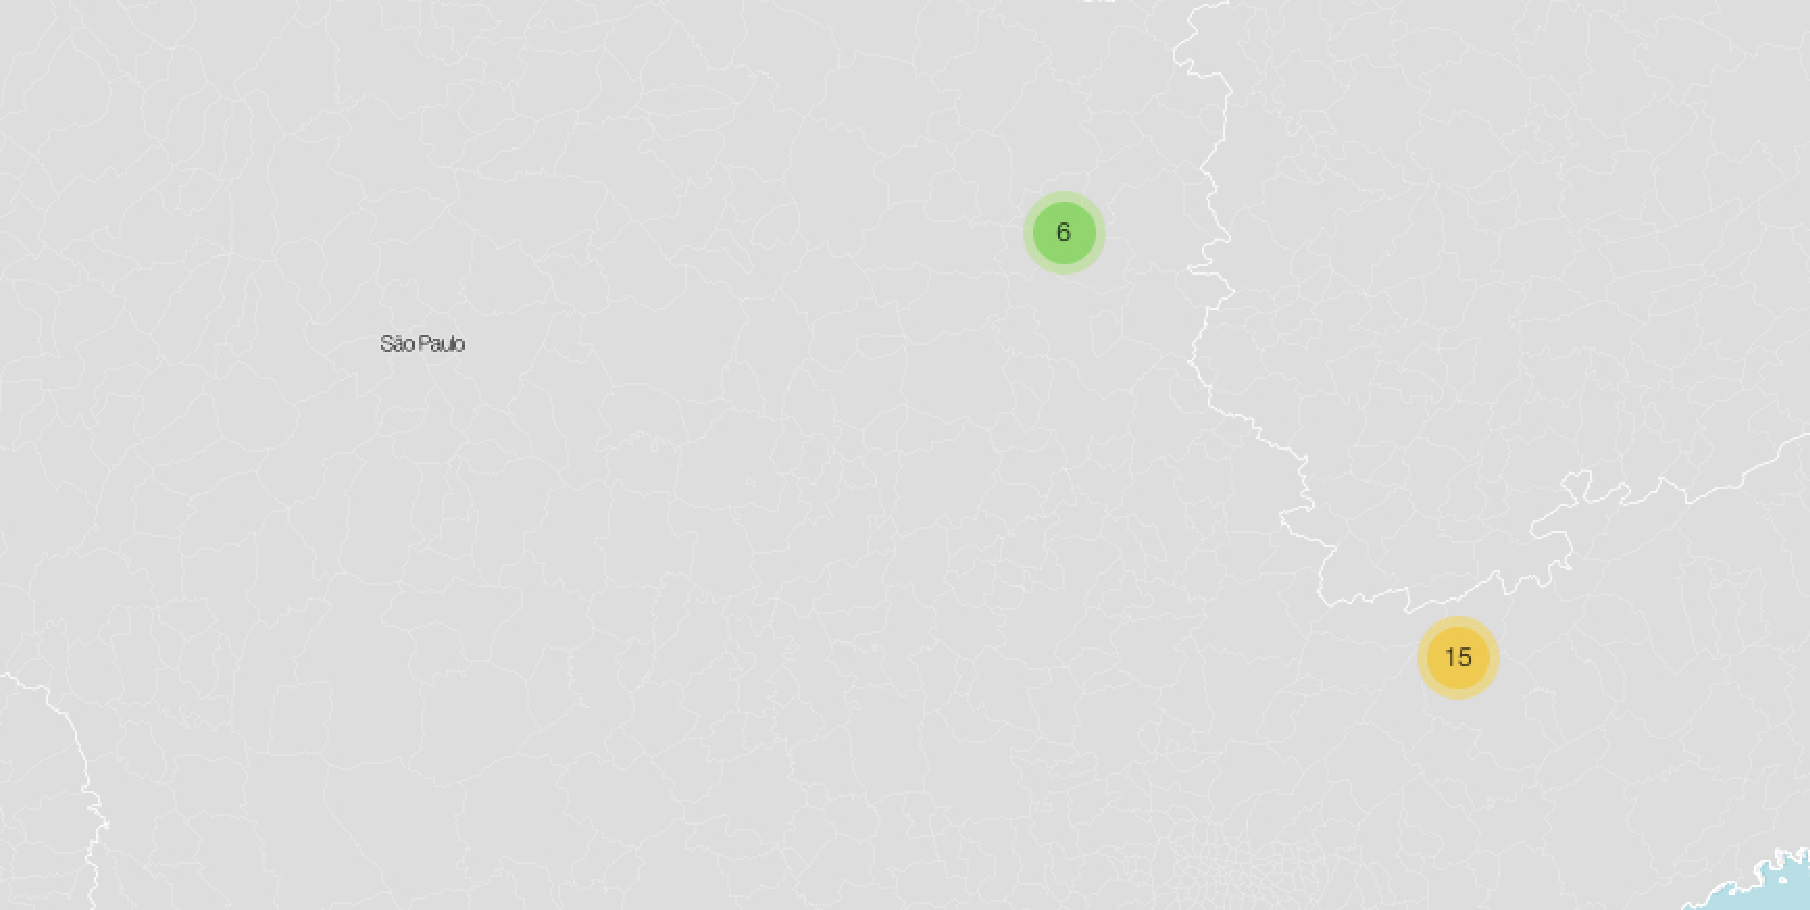
\includegraphics[width=1.0\textwidth]{figuras/mapa-marcador-2.pdf}
  \caption{Concentração de publicações em São Paulo.}
  \end{center}
\end{figure}

Antes, as 27 publicações que agrupadas em determinada área, através da ampliação do mapa se diviram em áreas menores, sendo as maiores delas 15 publicações e outra com 6 publicações. Tal informação indica dois polos distintos de surgimento de publicações, o que pode indicar a ocorrência de dois eventos distintos ou não.

Ao amplificar mais uma vez o mapa, já é possível visualizar as publicações de forma única, como indica a Figura 5.9.

\begin{figure}[h!]
  \begin{center}
  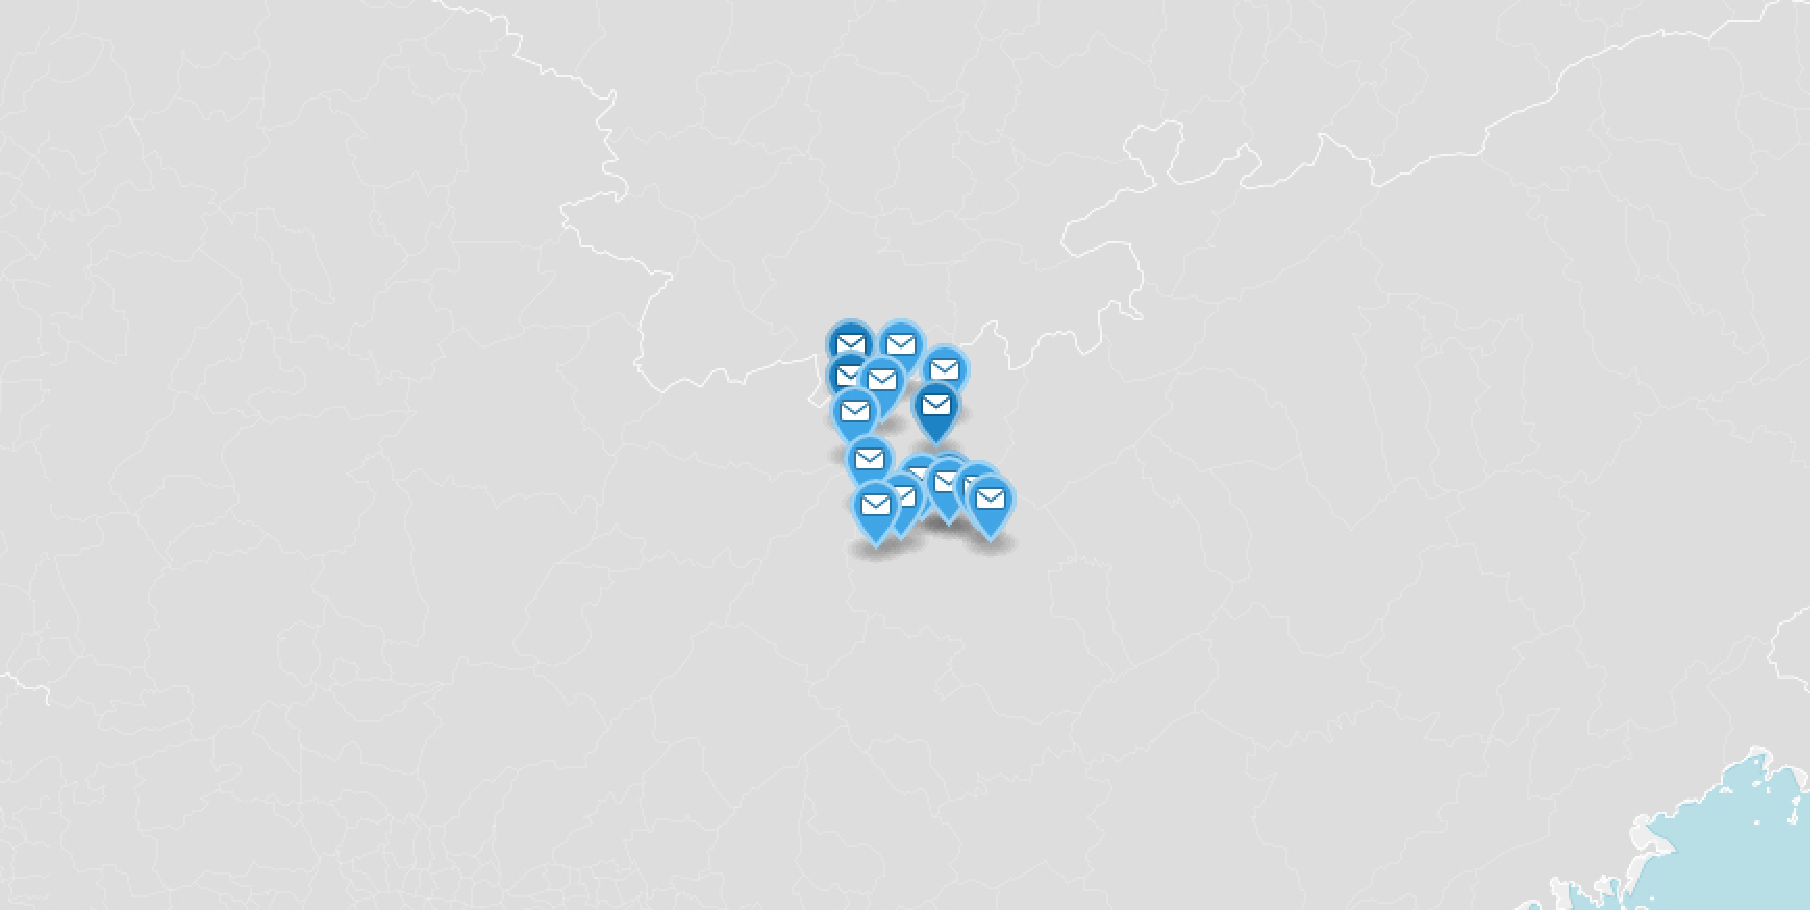
\includegraphics[width=1.0\textwidth]{figuras/mapa-marcador-3.pdf}
  \caption{Publicações únicas em São Paulo.}
  \end{center}
\end{figure}

É possível perceber que, nesse horário, um grande número de publicações está surgindo dessa região de São Paulo. Para obter detalhes e descobrir ao que se refere essa concentração de publicações repentina em determinada localização, é possível clicar em cada marcador e exibir a sua mensagem, como indica a Figura 5.10.

\begin{figure}[h!]
  \begin{center}
  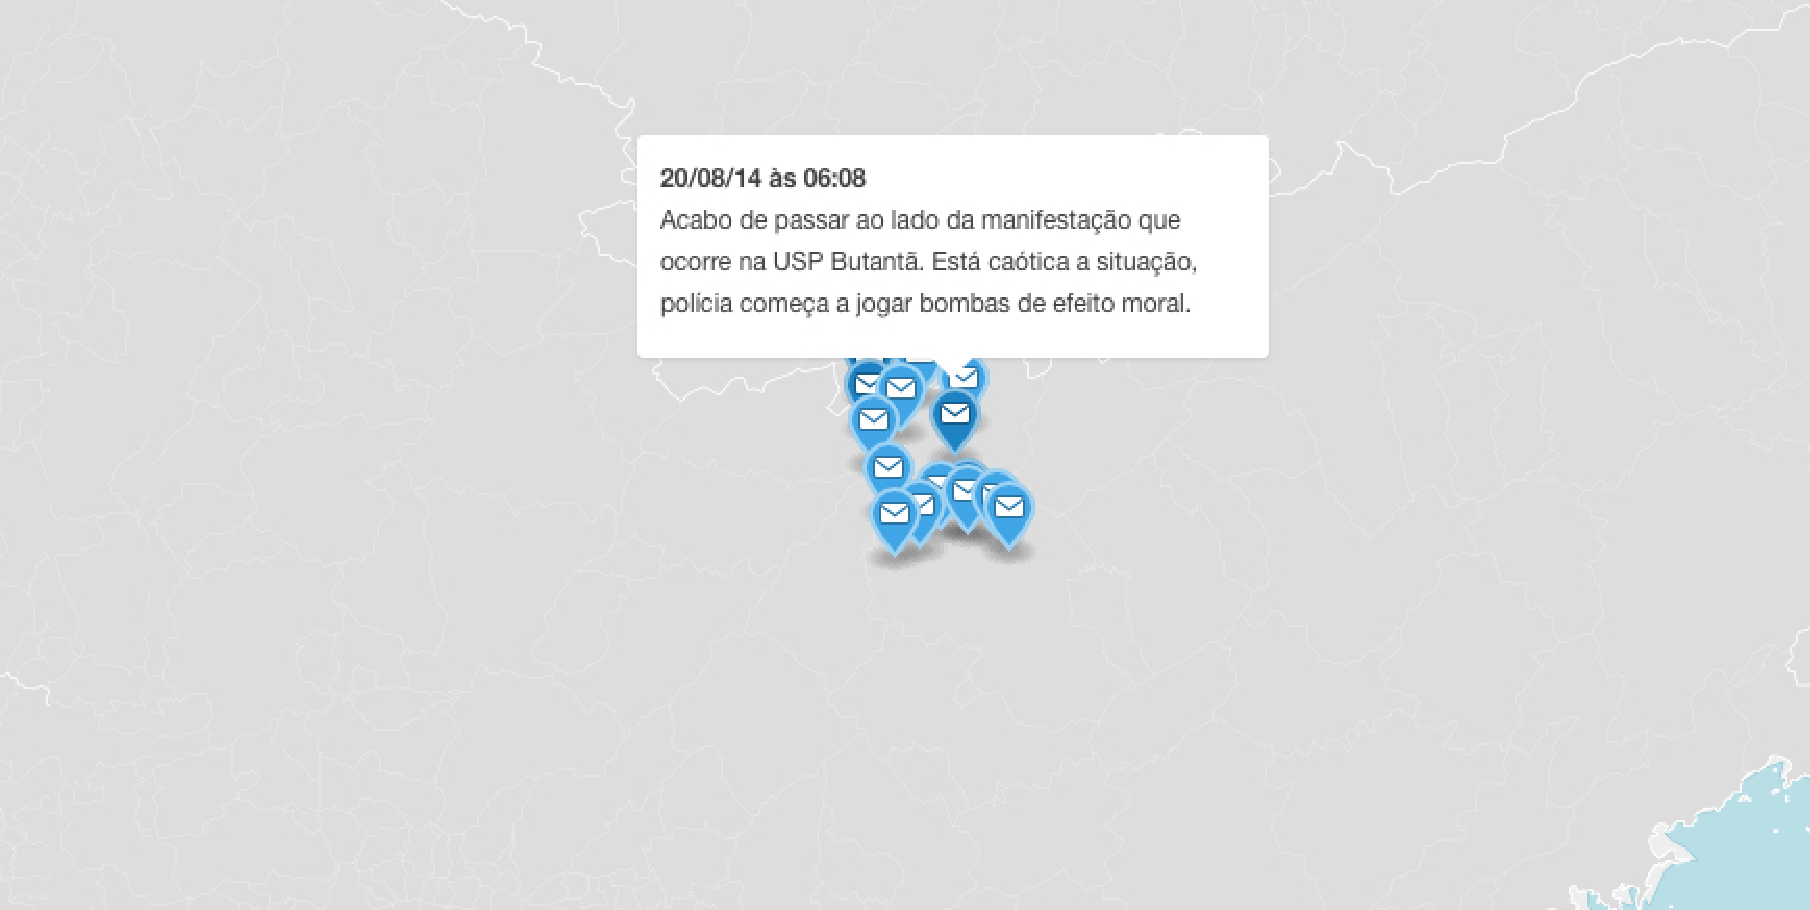
\includegraphics[width=1.0\textwidth]{figuras/mapa-marcador-4.pdf}
  \caption{Agrupamentos de publicações em Minas Gerais e São Paulo.}
  \end{center}
\end{figure}

Através da mensagem da publicação, é possível identificar sobre qual evento a concentração se refere. Nesse caso, o evento em questão foi a ocorrência de uma manifestação no campos da USP Butantã (Universidade de São Paulo), o que gerou a erupção de publicações naquela localização e horário.

Há ainda, os picos de publicações das faixas 17h-18h e 19h-20h do dia 20 de agosto, apresentados na Figura 5.4. A faixa entre 17h e 18h exibe grande concentração do estado de Minas Gerais e uma menor concentração em São Paulo, como indica a Figura 5.11. 

\begin{figure}[h!]
  \begin{center}
  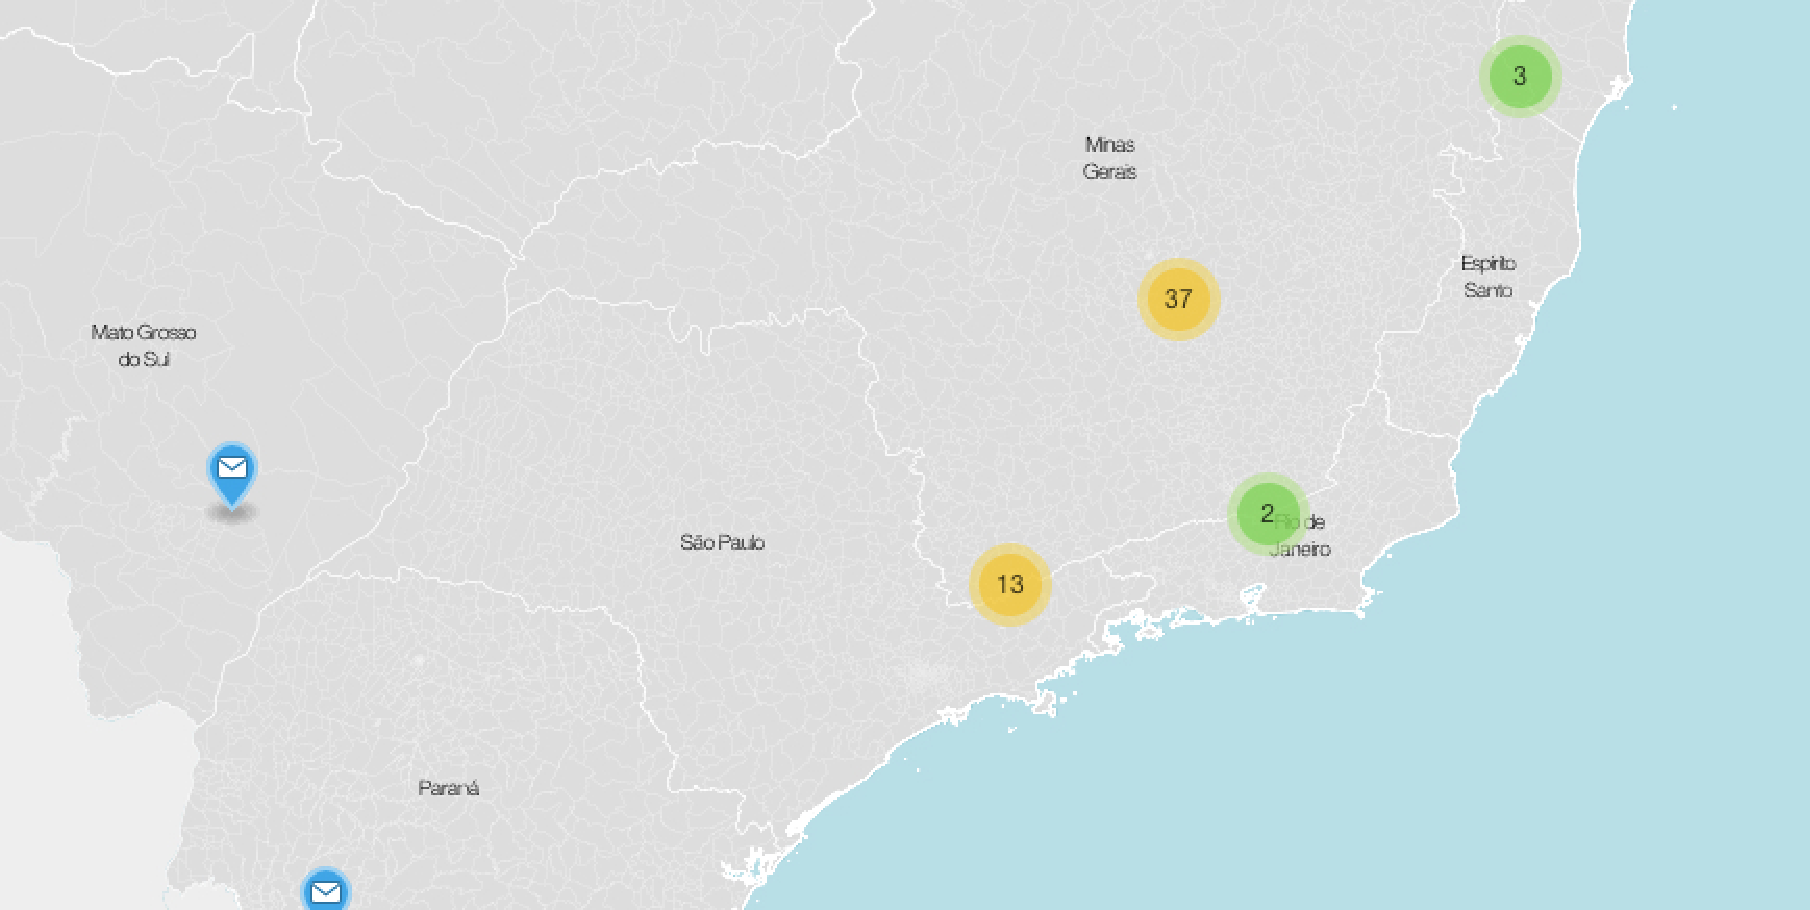
\includegraphics[width=1.0\textwidth]{figuras/mapa-marcador-6.pdf}
  \caption{Mensagem de uma publicação.}
  \end{center}
\end{figure}

Ao ampliar o mapa, é possível identificar dois eventos nessa faixa de horário: uma manifestação que interditou a rodovia MG-040 por volta das 17h40, e outra em frente ao Masp, na Avenida Paulista. Como indicam a Figura 5.12 e 5.13:

\begin{figure}[h!]
  \begin{center}
  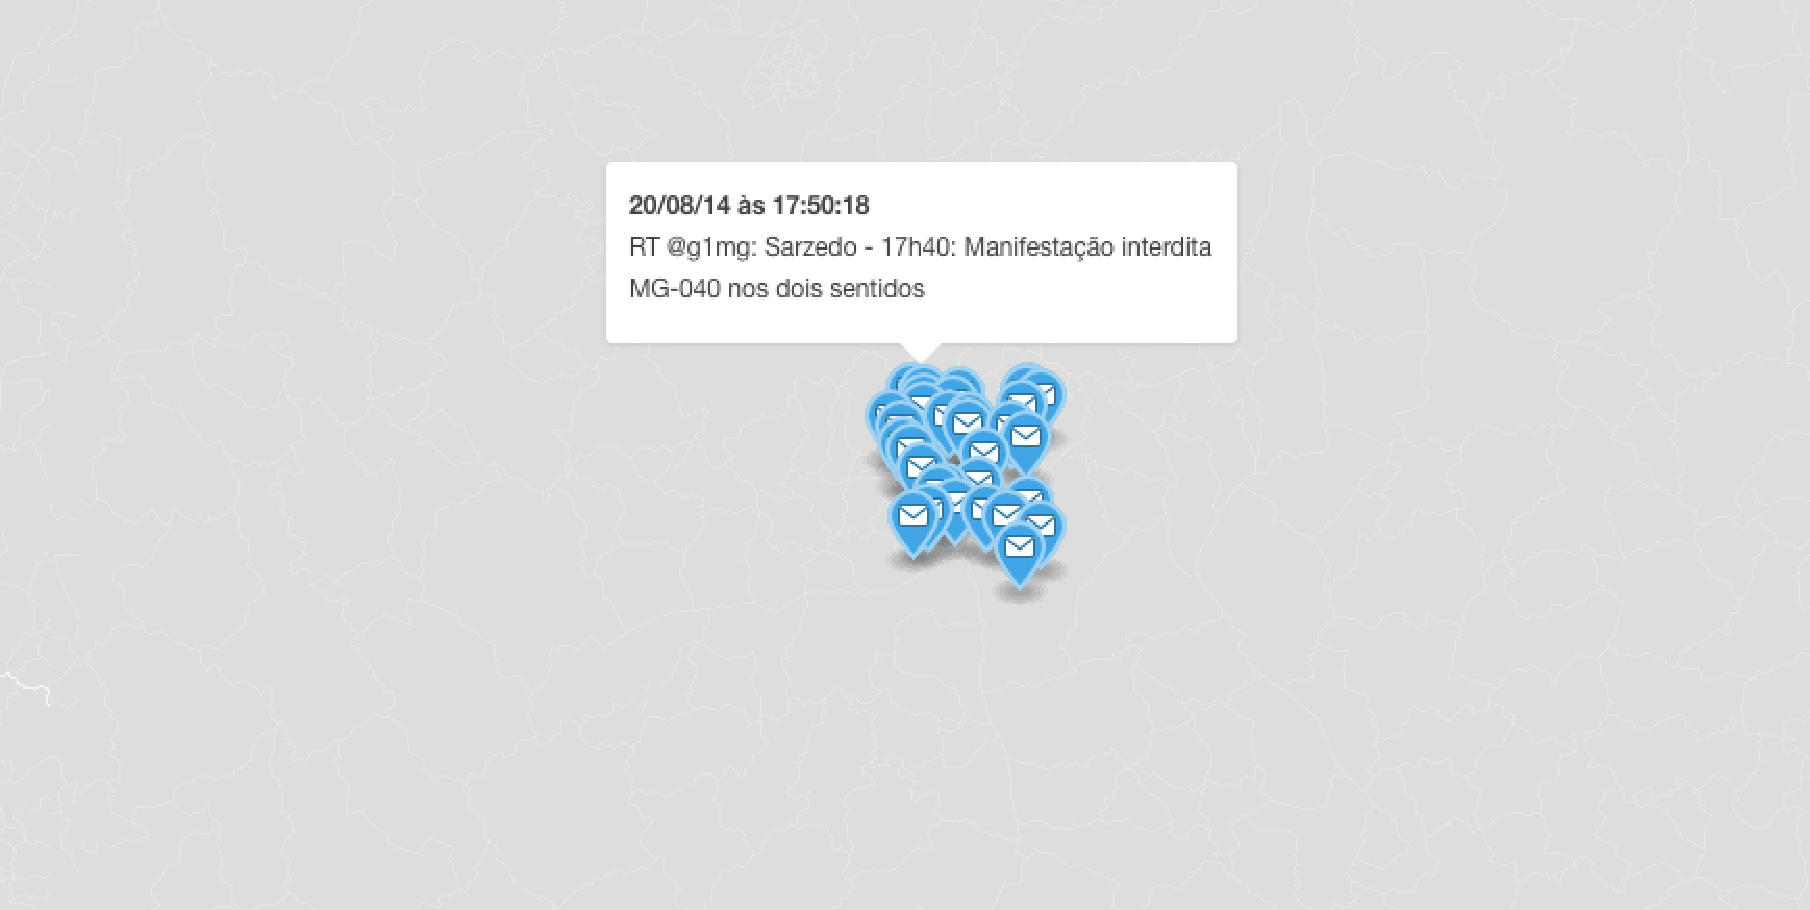
\includegraphics[width=1.0\textwidth]{figuras/mapa-marcador-5.pdf}
  \caption{Manifestação na rodovia MG-040, em Minas Gerais.}
  \end{center}
\end{figure}

\begin{figure}[h!]
  \begin{center}
  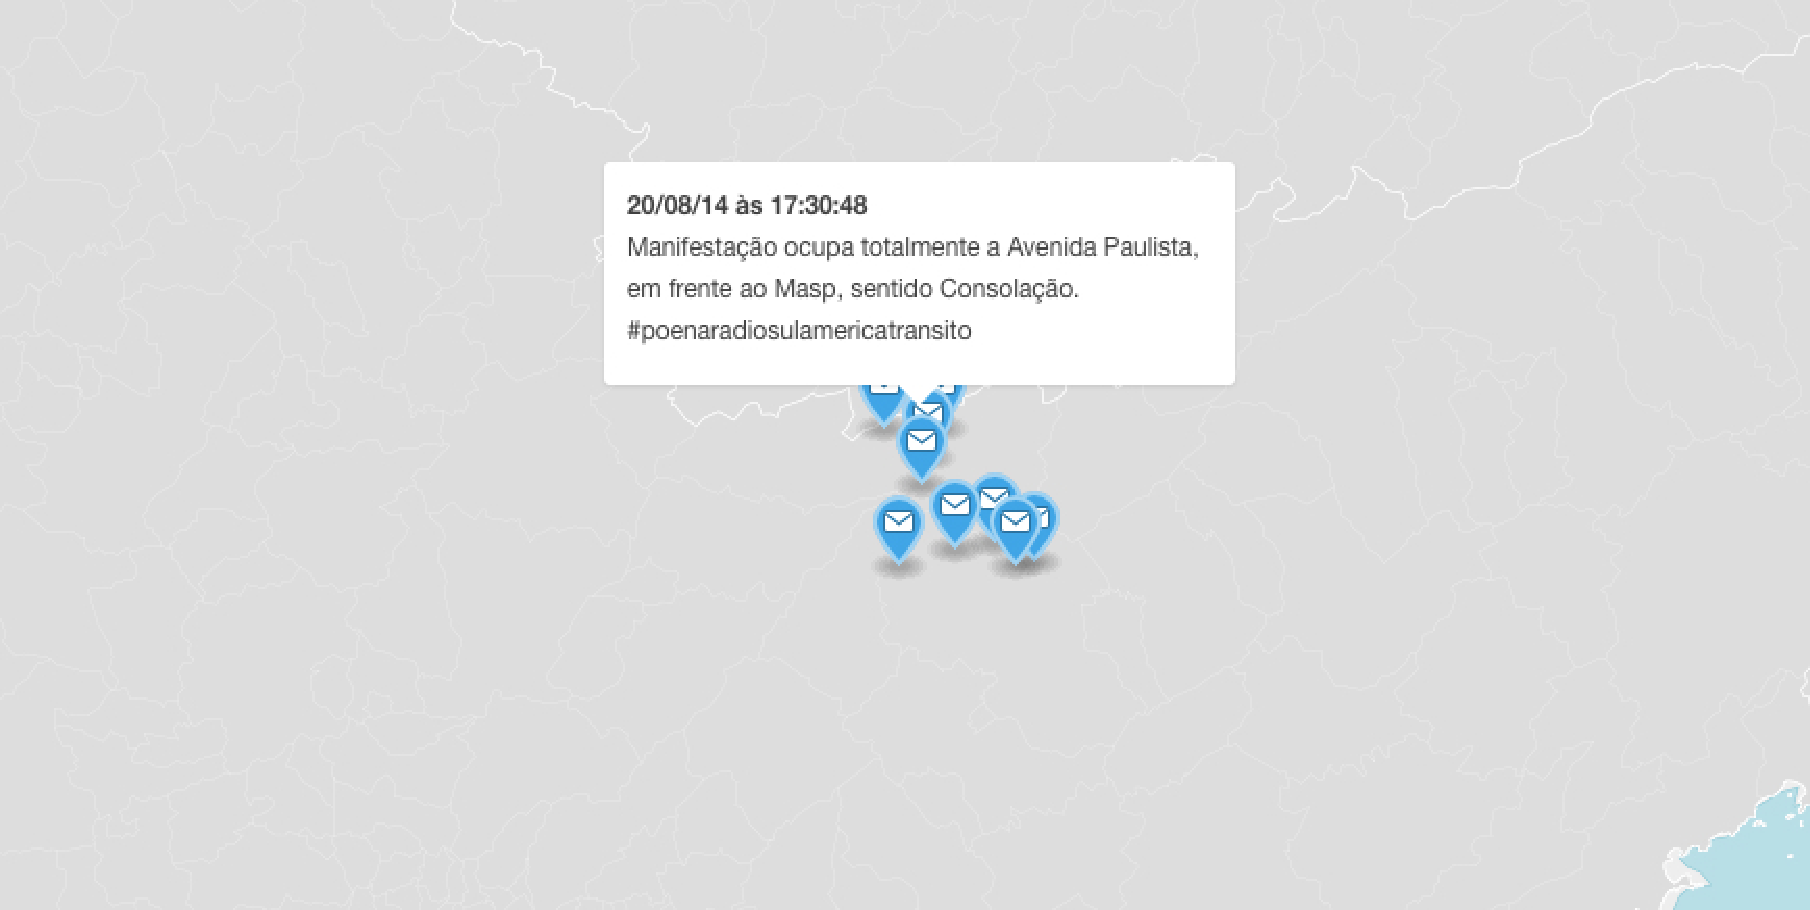
\includegraphics[width=1.0\textwidth]{figuras/mapa-marcador-7.pdf}
  \caption{Manifestação na Avenida Paulista, em São Paulo.}
  \end{center}
\end{figure}

A análise desse dia em específico mostra que o modelo, através de dados esparsos e desordenados em formato de texto, organiza essas informações e as apresenta em um ambiente que permite a análise visual de informações relevantes como o evento ocrrido, a localização aproximada e o seu horário.

% \subsection*{Análise da frequência de termos}

% Para visualizar a frequência dos termos contidos nas publicações de manifestações, é criada uma nuvem de termos, a partir da ferramente JQCloud\footnote{https://github.com/lucaong/jQCloud}. São inseridas as palavras e a sua frequência e a ferramenta gera uma nuvem com os termos mais frequentes em escala maior e vice-versa. Na Figura 5.5 está exibida a nuvem de termos gerada:

% \begin{figure}[h!]
%   \begin{center}
%   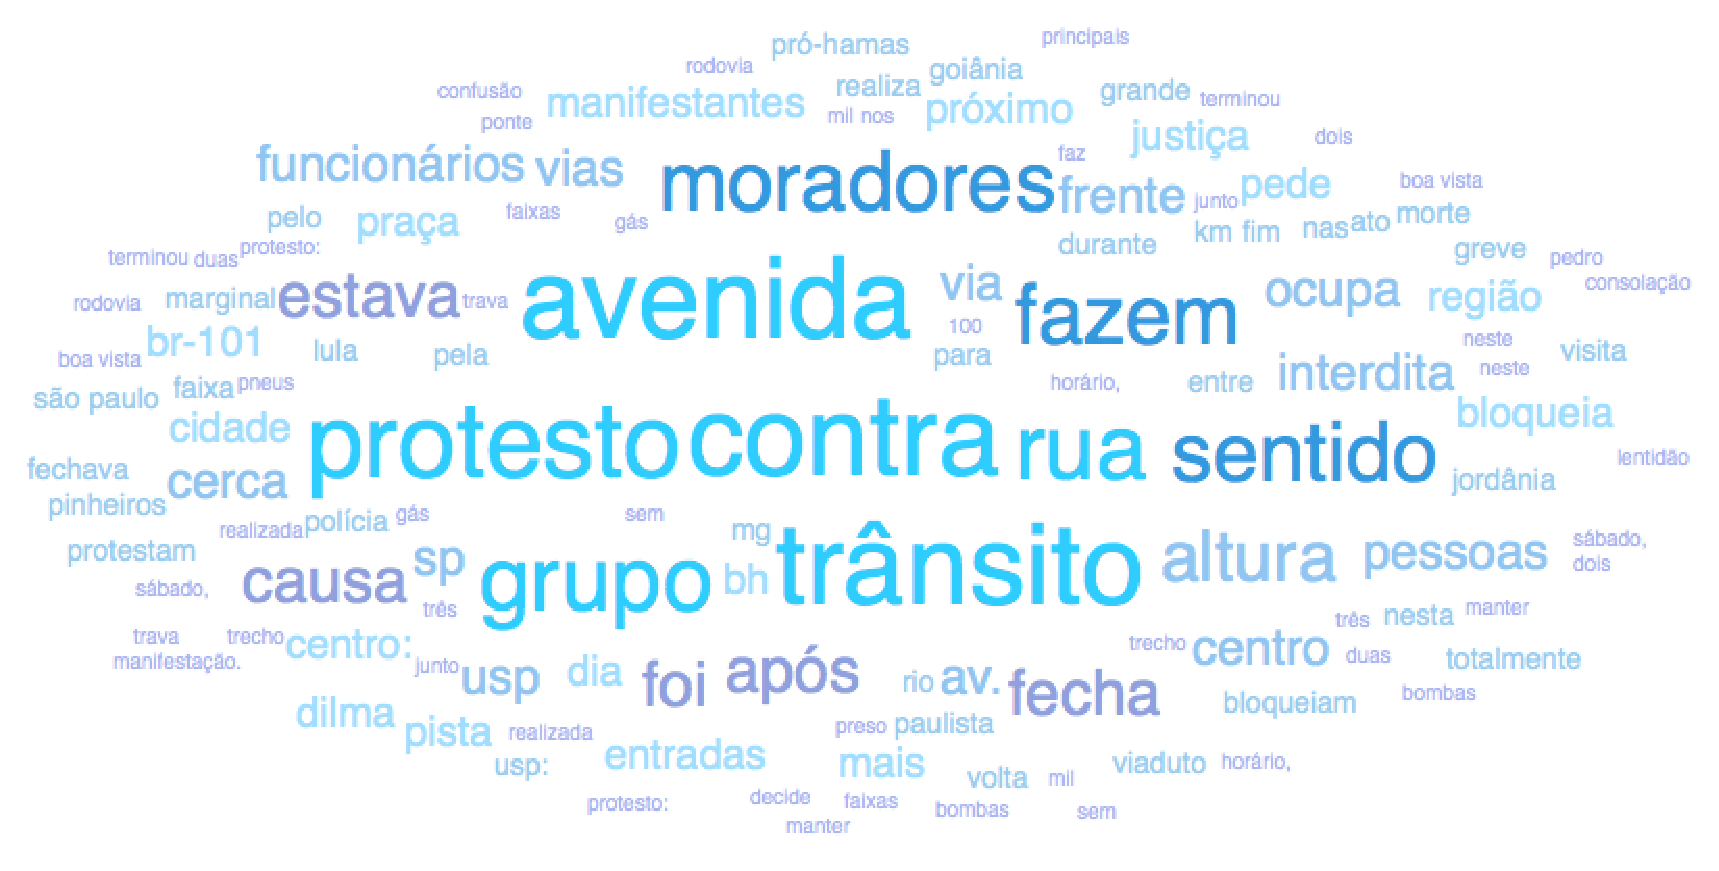
\includegraphics[width=1.0\textwidth]{figuras/nuvem-palavras.pdf}
%   \caption{Nuvem de palavras mais recorrentes.}
%   \end{center}
% \end{figure}

% É possível ver que os termos ``contra'', ``trânsito'', ``avenida'', ``protesto'' e ``grupo'' foram as mais recorrentes nas publicações de manifestações, o que reflete a realidade conhecida. Eventos de manifestações geralmente estão ligados à interdição de avenidas e do trânsito, e são criadas por grupos, contra um determinado objeto.
\chapter{Conclusão}

Junto com outros trabalhos que obtiveram sucesso ao detectar outros eventos com dados do Twitter, como o de \citeonline{Sakaki2010}, que detecta terremotos e \citeonline{Mai2012}, que detecta acidentes de trânsito, o modelo implementado apresentou que é possível a detecção de manifestações através dos dados obtidos do serviço. Manifesação é um acontecimento com certa escala, de importância na vida das pessoas e que possui local e horário, o que possibilita a sua detecção, pois, os usuários ao tomarem conhecimento de uma manifestação, rapidamente publicam sobre ela, gerando picos de publicações que podem ser observados através dos gráficos de série-temporal.

A classificação com SVM utilizou um conjunto de dados de treino do SVM de cerca de 1\% dos dados totais, e obteve cerca de 90\% de taxa de acerto, produzindo resultado relevante e permitindo que, a partir de uma pequena gama de amostras, o conjunto completo dos dados fosse classificado com baixa margem de erro. O ajuste do parâmetro $C$ apresentou comportamento esperado. Ao incrementá-lo ou decrementá-lo demais, a taxa de acerto diminuia, sendo necessário, através de testes sucessivos, encontrar um valor mediano que apresentasse o melhor resultado.

Ao analisar os gráficos de série-temporal através do ambiente interativo, foi possível identificar as erupções repentinas de publicações, e que as mesmas dizem respeito à um ou mais evento específicos. Quando há um repentino surgimento de muitas publicações em determinada faixa de horário, elas geralmente possuem conteúdo convergente sobre um mesmo evento. Mostrando um motivo claro para a erupção de publicações: a ocorrência de um ou mais novos eventos.

Através da análise do mapa de marcadores foi possível identificar, aproximadamente, a localização dos eventos através da posição dos marcadores no mapa e o seu agrupamento. Também identificou-se sobre qual evento as publicações estão se referindo, através da visualização das suas mensagens.

\section{Dificuldades}

A principal dificuldade encontrada durante a implementação detecção de eventos com dados do Twitter foi o limite de busca imposto pelo serviço. Inicialmente, era pretendido coletar publicações dentro de um período de dois anos, porém, o Twitter exibe a restrição de busca para publicações criadas apenas até uma semana. Com isso, a busca foi restrita ao mês de Agosto de 2014, sendo necessária a realização de várias buscas em datas diferentes e a concatenação dos resultados no mesmo arquivo.

\section{Trabalhos futuros}

O modelo implementado ainda não consegue estimar de forma automática se, em um determinado momento no tempo, está ocorrendo um evento ou não, ou seja, se a quantidade de publicações em determinada faixa de horário é normal ao funcionamento do sistema ou de fato anômala. 

Isso seria possível através da implementação de um modelo probabilístico, que se encarregaria de analisar à qual tipo de distribuição probabilística os dados se enquadram. Seria feita então a comparação entre a distribuição e os dados reais obtidos. Caso haja divergência acima de uma limiar estabelecido, naquele momento estaria ocorrendo um evento.

O modelo também ainda não estima a localização de um evento. Com implementação dos métodos de filtros de Kalman ou de particulas, seria possível, através das informações de localização das publicações, estimar o local de ocorrência de um evento. Essa estimativa, porém, possui a complexidade da determinação de quais publicações se referem ao evento em questão, pois é possível que, na mesma faixa de horário, haja a erupção de publicações sobre dois eventos distintos.
\appendix

\chapter{Código do modelo}

\section{Classificador}

Classe utilizada as ações referentes à classificação das publicações.

\begin{lstlisting}
	require 'csv'
	require 'libsvm'

	class Classificador
		attr_reader :problema, :parametro, :termos_excecao, :treinador, :modelo, :publicacoes

		def initialize
			@problema = Libsvm::Problem.new
			@parametro = Libsvm::SvmParameter.new
			@treinador = Treinador.new
			@publicacoes = []
			inicializa_parametros
		end

		def inicializa_parametros
			@parametro.c = 0.1
			@parametro.cache_size = 1
			@parametro.eps = 0.001
		end

		def carregar_publicacoes_de_treino caminho
			@treinador.carregar_publicacoes_de_treino caminho
		end

		def definir_modelo
			@problema.set_examples(@treinador.classes, @treinador.vetores_de_treino)
			@modelo = Libsvm::Model.train(@problema, @parametro)
		end

		def carregar_publicacoes caminho
			CSV.open(caminho) do |csv|
				csv.each do |linha|
					@publicacoes << Publicacao.new(linha, @treinador)
				end
			end
		end

		def testar_modelo caminho_saida
			definir_modelo
			CSV.open(caminho_saida, "w") do |csv|
				@publicacoes.each do |publicacao|
					linha_csv = publicacao.linha_csv
					classe = @modelo.predict(publicacao.vetor)
					linha_csv[6] = classe
					linha_csv[7] = publicacao.cidade
					linha_csv[8] = publicacao.estado
					csv << linha_csv
				end
			end
		end
	end
\end{lstlisting}

\section{Publicação}

Classe utilizada para extração das informações das publicações como: termos, vetor de características, cidade e estado.

\begin{lstlisting}
	class Publicacao
	  attr_reader :termos, :vetor, :linha_csv, :texto, :horario, :latitude, 
	  	:longitude, :cidade, :localizacao_no_perfil

		def initialize linha, treinador = nil
			@linha_csv = linha
			@id = @linha_csv[0]
			@horario = @linha_csv[1]
			@texto = @linha_csv[2]
			@latitude = @linha_csv[3]
			@longitude = @linha_csv[4]
			@localizacao_no_perfil = @linha_csv[5]
			@treinador = treinador
			@termos = @texto.tokenizar
			@cidade = extrair_cidade
		end

		def extrair_cidade
			cidade = ""
			@termos.each do |termo|
				if String::LISTA_DE_CIDADES.include?(termo)
					cidade = termo
				end
			end
			if cidade == "" && @localizacao_no_perfil
				@localizacao_no_perfil.tokenizar.each do |termo|
					if String::LISTA_DE_CIDADES.include?(termo)
						cidade = termo
					end
				end
			end
			cidade
		end

		def estado
			String::ESTADOS_E_CIDADES[@cidade]
		end

		def vetor
			if @treinador
				vetor = @treinador.dicionario_de_termos.map do |termo| 
					@termos.include?(termo) ? 1 : 0
				end
				Libsvm::Node.features(vetor)
			end
		end
	end
\end{lstlisting}

\section{Treinador}

Classe utilizada para a fase de treinamento do classificador e criação do dicionário de termos.

\begin{lstlisting}
	class Treinador
		attr_reader :publicacoes_de_treino, :publicacoes_de_teste, :dicionario_de_termos

		def initialize
			@publicacoes_de_treino = []
		end

		def carregar_publicacoes_de_treino caminho
			CSV.open(caminho) do |csv|
				csv.each do |linha|
					@publicacoes_de_treino << Publicacao.new(linha, self)
				end
			end
			criar_dicionario_de_termos
		end

		def criar_dicionario_de_termos
			@dicionario_de_termos = @publicacoes_de_treino.map do |publicacao| 
				publicacao.termos
			end.flatten.uniq.sort
		end

		def classes
			@publicacoes_de_treino.map { |publicacao| publicacao.linha_csv[6].to_i }
		end

		def vetores_de_treino
			@publicacoes_de_treino.map { |publicacao| publicacao.vetor }
		end
	end
\end{lstlisting}

\section{Twitter}

Classe utilizada para obter as publicações do Twitter.

\begin{lstlisting}
	require 'twitter'

	class Twitter
		def initialize
			@cliente = Twitter::REST::Client.new do |config|
			  config.consumer_key        = "DbT8fYWR2jq1TIXvxVtiZzFno"
			  config.consumer_secret     = "3mT9JcwgaWs5gTJqOihbGAlRplHTKQapJMNQtnAWufYMVyUmle"
			  config.access_token        = "42659961-4wDJCea7t1KVf1FMqUK5H2k2zgBaE26GpI5kjC3CK"
			  config.access_token_secret = "OjhVszJ3Dyivaz0gGhHUuKn5N7cYqE0jUinoaFiWK7FjY"
			end
		end

		def buscar data_limite, expressao, caminho_arquivo
			data_publicacao = Time.now
			id_maximo = nil

			while publication_date > data_limite
				publicacaoes = @cliente.search(expressao, lang: "pt", max_id: id_maximo).to_a
				data_publicacao = publicacaoes.last.created_at
				id_maximo = publicacoes.last[:id] - 1
				CSV.open(caminho_arquivo, "a+") do |csv|
					publicacoes.each do |publicacao| 
						csv << [publicacao[:id], publicacao.created_at, publicacao.text, publicacao.geo.latitude, publicacao.geo.longitude, publicacao.user.location]
					end
				end
			end
		end
	end
\end{lstlisting}

\section{String}

Sobrecarga da classe String nativa do Ruby para manipulação das cidades e tokenização das publicações.

\begin{lstlisting}
	require 'json'

	class String
		JSON_CIDADES = JSON.parse(IO.read("support/cidades_do_brasil.json"))
		ESTADOS_E_CIDADES = JSON_CIDADES.each_with_object({}) do |(k,v), h|
			h[k.downcase] = v.downcase
		end
		LISTA_DE_CIDADES = ESTADOS_E_CIDADES.keys.sort_by { |c| c.length }.reverse
		CIDADES_UNIDAS = LISTA_DE_CIDADES.map { |city| "(\\b#{city}\\b)" }.join("\|")
		CIDADES_EXPREG = Regexp.new "#{CIDADES_UNIDAS}|\\s"
		EXCECOES = [
			"a", "e", "o", "de", "do", "da", "dos", "das", 
			"os", "as", "se", "meu", "que", "teu", "ou", "eu",
			"é", "à", "um", "uma", "uns", "umas", "RT"
		]

		def tokenizar
			termos = self.downcase.split(CIDADES_EXPREG).map! { |termo| termo.gsub(/\p{^Alnum}\s/, '') }
			termos.delete_if do |termo| 
			  termo == "" || EXCECOES.include?(termo) || termo.include?("http") || 
			  termo.include?("@") || termo.include?("kk") || termo.include?("haha")
			end
		end
	end
\end{lstlisting}

\section{Modelo}

Programa principal que realiza as chamadas na ordem (a obtenção das publicações com a classe Twitter é executada separadamente).

\begin{lstlisting}
	["classificador", "publicacao", "string", "treinador"].each do |file|
		require "./lib/#{file}.rb"
	end

	classificador = Classificador.new
	classificador.carregar_publicacoes_de_treino "support/publicacoes_de_treino.csv"
	classificador.carregar_publicacoes "support/publicacoes.csv"
	classificador.testar_modelo "support/publicacoes_classificadas.csv"
\end{lstlisting}

%--------------------------------- Bibliografia --------------------------------

\citeoption{abnt-repeated-author-omit=yes}
\bibliographystyle{abnt-alf}
\bibliography{bibliografia}

\end{document}

